\documentclass{article}
\usepackage{aaai}

\usepackage{helvet}
\usepackage{rotating}
\usepackage{graphicx}
\usepackage{subfigure}
\usepackage{hyperref} 
\usepackage[linesnumbered,ruled,vlined]{algorithm2e}


\renewcommand\floatpagefraction{1} \renewcommand\topfraction{1}
\renewcommand\bottomfraction{1} \renewcommand\textfraction{0}
\renewcommand{\dbltopfraction}{1} \renewcommand{\dblfloatpagefraction}{1}
\setcounter{totalnumber}{50} \setcounter{topnumber}{50}
\setcounter{bottomnumber}{50} \setcounter{dbltopnumber}{50}

% \setcounter{page}{1}
\def\citep#1{\cite{#1}} \def\citet#1{\citeA{#1}}


\usepackage{amsmath, amsthm, amssymb}


% \usepackage{cite} \usepackage{amsfonts} \usepackage{graphicx}
% \usepackage{cite}
\usepackage{natbib,natbibspacing}
\setlength{\bibspacing}{0}

\usepackage{multirow}
\def\und#1{\noindent{\bf #1}:}

% \def\citep#1{(\citeauthor{#1}, \citeyear{#1})} \def\citet#1{\citeauthor{#1}
% (\citeyear{#1})}
\newtheorem{theorem}{Theorem}[section]
\newtheorem{lemma}[theorem]{Lemma}
\newtheorem{proposition}[theorem]{Proposition}
\newtheorem{corollary}[theorem]{Corollary}
\newtheorem{definition}[theorem]{Definition}


   % General parameters, for ALL pages:
   \renewcommand{\topfraction}{0.9} % max fraction of floats at top
   \renewcommand{\bottomfraction}{0.8} % max fraction of floats at bottom
    % Parameters for TEXT pages (not float pages):
% \setcounter{topnumber}{2}
   % \setcounter{bottomnumber}{2}
    % \setcounter{totalnumber}{4}     % 2 may work better
    % \setcounter{dbltopnumber}{2}    % for 2-column pages
    % \renewcommand{\dbltopfraction}{0.9} % fit big float above 2-col. text
    % \renewcommand{\textfraction}{0.07} % allow minimal text w. figs Parameters
    % for FLOAT pages (not text pages): \renewcommand{\floatpagefraction}{0.7} %
    % require fuller float pages
	% N.B.: floatpagefraction MUST be less than topfraction !!
   \renewcommand{\dblfloatpagefraction}{0.7} % require fuller float pages


\newenvironment{packed_enum}{
\begin{enumerate}
  \setlength{\itemsep}{1pt}
  \setlength{\parskip}{0pt}
  \setlength{\parsep}{0pt}
}{\end{enumerate}}

\newenvironment{packed_itemize}{
\begin{itemize}
  \setlength{\itemsep}{1pt}
  \setlength{\parskip}{0pt}
  \setlength{\parsep}{0pt}
}{\end{itemize}}


\usepackage{ifthen}
\newboolean{USEEXAMPLE}
\setboolean{USEEXAMPLE}{true}


\def\baselinestretch{.99}

%\usepackage{natbibspacing}
%\setlength{\bibspacing}{.1\baselineskip}


\def\FFRISKY{{\tt DeFAULT}}
\def\default{{\tt DeFAULT}}
\def\goalie{{\tt Goalie}}





%%%%%%%%%%%%%%%%%%%%%%%%%%%%%%%%%%%%%%%%

%
%
%\input epsf
%\usepackage{times}
%\usepackage{courier}
%\usepackage{latexsym}
%\usepackage{amsmath, amssymb}
%\usepackage{epic}
%\usepackage{eepic}
%\usepackage{graphics}


\def\bold#1{{#1}}
\def\und#1{\medskip{\noindent\bf #1:}}




\begin{document}

\title{Planning and Acting in Incomplete Domains
% \thanks{Extended Technical Report Available at: \
% \href{http://www.cs.usu.edu/~danbryce/papers/USU-CS-TR-11-001.pdf}{
% http://www.cs.usu.edu/$\sim$danbryce/papers/USU-CS-TR-11-001.pdf}}
}

\author{%Paper \#114}
Christopher Weber and Daniel Bryce\\
christopherweber@hotmail.com, daniel.bryce@usu.edu\\
Department of Computer Science\\
Utah State Univeristy
}

%%%%%%%%%%%%%%%PS/PDF%%%%%%%%%%%%%%%%%%%
%\author{\name Daniel Bryce \email daniel.bryce@usu.edu\\
%\name Jared Robertson \email jared.robertson@usu.edu\\
%\addr Department of Computer Science\\
% Utah State University\\
% 4205 Old Main Hill, Logan, UT 84321}
%%%%%%%%%%%%%%%%%%%%%%%%%%%%%%%%%%%%%%%%


%1 Intro
%1 Model
% 1 Diagnosis
% 0.5 Filtering
% 1.5 Planning
% 2 Results
% 1 Conclusion, Related, References

\maketitle

\begin{abstract}
Engineering complete planning domain descriptions is often very costly because
of human error or lack of domain knowledge. Learning complete domain
descriptions is also very challenging because many features are irrelevant to
achieving the goals and data may be scarce.  We present an agent that plans and
acts in incomplete domains by i) synthesizing plans to avoid execution failure
due to ignorance of the domain model, and ii) passively learning about the
domain model during execution to improve later re-planning attempts.

Our planner \default{} is the first to reason about a domain's incompleteness to
avoid potential plan failure.  \default{} computes failure explanations for each
action and state in the plan and counts the number of interpretations of the
incomplete domain where failure will occur. We show that \default{} performs
best by counting  prime implicants (failure diagnoses) rather than propositional
models. Our agent \goalie{} learns about the preconditions and effects of
incompletely-specified actions while monitoring its state and, in conjunction
with \default{} plan failure explanations, can diagnose past and future action
failures.   We show that by reasoning about incompleteness in planning (as
opposed to ignoring it) \goalie{} re-plans less, executes fewer actions, and
achieves its goals faster.

%\goalie{} and \default{} intentionally circumvent domain incompleteness as much as possible to achieve a problem's goals, but 

%an execution strategy is novel in that it does not assume that the environment provides perfect feedback about failed actions, and that it can determine early if a plan will fail. Our planner, DeFault, reasons about incompleteness by computing failure explanations as Boolean sentences and counting propositional models to bias plan search.  We evaluate a number of alternative representations and counting approaches, and find that counting prime implicants (not models) can lead to scale-up in complex domains.  We also show that reasoning about incompleteness, instead of ignoring it, leads to more effective agents that take less time, actions, and re-planning episodes to achieve their goals.

%We evaluate both planning and execution on a number of domains 
%
%While many have studied knowledge acquisition, relatively few have studied the synthesis of plans when the domain model is incomplete (i.e., actions have incomplete preconditions or effects).  Prior work has evaluated the correctness of plans synthesized by disregarding such incomplete features, but not how to synthesize plans by reasoning about the incompleteness.  In this work, we describe several techniques for reasoning with the action incompleteness to increase the number of interpretations under which the plans will succeed.  Among the techniques, we show that representing explanations of plan failure with prime implicants provides a natural approach to comparing plans by counting prime implicants instead of models -- leading to better scalability and comparable quality plans.
%
%We present and empirically evaluate a forward heuristic search planner, called \FFRISKY{}, that synthesizes plans by propagating information about faults due to incompleteness both within the state space and the relaxed planning space.  We also provide a translation from incomplete planning domains to conformant probabilistic planning, where action incompleteness is represented by state incompleteness.  We compare \FFRISKY{} with a control planner that uses the FF heuristic (measuring plan length and ignoring incompleteness), and with the conformant probabilistic planner POND.  The results show that \FFRISKY{} i) scales better than POND, ii) scales comparable to the planner using the FF heuristic (while finding better solutions), and iii) scales better when counting prime implicants than models.
%
%%several relaxed plan heuristics that measure fault.  The most simple heuristic computes a relaxed plan with no notion of fault, but measures the fault of this relaxed plan.  The second heuristic involves propagating measures of plan fault and using the fault measure to bias the relaxed plan.  The last measure encodes the relaxed planning problem as an integer program to compute the minimal fault.  We compare each of these heuristics to a planner that counts the actions in the relaxed plan as its heuristic gauge the improved plan quality with respect to fault.

\end{abstract}


\section{Introduction}
%    %Planning with incomplete domains is important in applications (incl BL)
The knowledge engineering required to create complete and correct domain
descriptions for planning problems is often very costly and difficult
\citep{modellite,arms}.  Machine learning techniques have been applied with some
success \citep{arms}, but still suffer from impoverished data and limitations of
the algorithms \citep{modellite}.   In particular, we are motivated by
applications in instructable computing \citep{mable} where a domain expert
teaches an intelligent system about a domain, but can often leave out whole
procedures (plans) and aspects of action descriptions.   In such cases, the
alternative to making domains complete, is to plan around the incompleteness. 
That is, given knowledge of the possible action descriptions, we seek out plans
that will succeed despite any (or most) incompleteness in the domain
formulation.
%  %Prior work does not look at synthesis, just computes critical faults

While prior work \citep{Garland02} (henceforth abbreviated, GL) has categorized
risks to a plan and described plan quality metrics in terms of the risks
(essentially single-fault diagnoses of plan failure \citep{dekleer}), no
prior work has sought to deliberately synthesize low-risk plans based on
incomplete STRIPS-style domains (notable work in Markov decision processes
\citep{NE:05}  and model-based reinforcement learning \citep{citeulike:112017}
has explored similar issues).  Our planner \default{} labels parital
plans with propositional explanations of failure due to incompleteness (derived
from the semantics of assumption based truth maintenance systems
\cite{USU-CS-TR-11-001}) and either counts failure models or prime implicants (diagnoses) to bias search.
% Specifically, \citet{Garland02}  identify four types of plan faults: open
% preconditions (due to incomplete preconditions), possible clobberers (due to
% incomplete delete effects), unlisted effects (due to incomplete add effects),
% and false preconditions.  GL develop an algorithm that steps backward through
% the plan to identify the ``critical faults'' -- those instances where
% incomplete domain features can cause plan failure.  For example, a possible
% clobber is a critical fault when (if it is truly a delete effect) it threatens
% a precondition or goal.  The number of critical faults is an important measure
% of plan quality/correctness, that, unfortunately, no known planners seek to
% minimize.
Our agent \goalie{} passively learns about the incomplete domain at it
executes actions, like \citet{DBLP:conf/aips/ChangA06} (henceforth
abbreviated, CA); however, unlike CA, \goalie{} executes plans that are robust
to domain incompleteness.  Within \goalie{}, we compare the use of robust plans
generated by our planner \default{}, and plans that are generated in the
spirit of CA which are not intentionally robust (i.e., optimistically
successful).  We demonstrate that the additional effort to synthesize robust
plans is justified because \default{} executes fewer overall actions, re-plans
less, and solves tasks in lower overall time.

% 
%  CA synthesize plans
% that will achieve the goals under any interpretation of the incomplete domain,
% however in doing so the planner can pick the most convenient interpretation and
% be overly optimistic.   Further, while operating in non-deterministic domains,
% they do not address learning action preconditions and assume that their
% environment will provide action failure signals.  We focus on deterministic
% environments, but lift their assumptions by learning preconditions and not
% relying on the environment signaling failure.

% Our planner \FFRISKY{} builds upon GL to synthesize plans robust to
% incompleteness and our agent \goalie{} builds upon CA to use robust plans while
% learning about all types of incomplete action features and diagnosing plan
% failure.  We rely on representing our knowledge of the incomplete domain and
% anticipated plan failure with propositional sentences that are manipulated
% during plan synthesis and execution.  The advantage of reasoning about the
% incompleteness in this fashion is that we can potentially avoid plan failure
% (i.e., unsatisfied (sub)goals), minimize re-planning, and often reduce overall
% planning and execution time over approaches that do not reason about
% incompleteness, such as the planner used by CA.

This paper is organized as follows.  The next section details Incomplete STRIPS,
the language we use to describe incomplete domains.  We follow with our approach
to plan synthesis and search heuristics.  We discuss alternatives to reasoning
about failure explanations, including model counting and prime implicant
counting.  We describe our execution monitoring and re-planning strategy, and
then provide an empirical analysis, related work, and conclusion.
  

%
%\und{Example} Consider the following action, that is taken from a modified version of the International Planning Competition (IPC) \citep{ipc5} PARC printer domain:  
%
%\begin{verbatim}
%(:action HtmOverBlack-Move-A4
% :parameters ( ?sheet - sheet_t )
% :precondition (and (clear) (Available HtmOverBlack-RSRC)
%                    (Sheetsize ?sheet A4) 
%                    (Location ?sheet HtmOverBlack_Entry-EndCap_Exit))
% :effect (and (not (Available HtmOverBlack-RSRC))
%              (Location ?sheet HtmOverBlack_Exit-Down_TopEntry)
%              (not (Location ?sheet HtmOverBlack_Entry-EndCap_Exit))
%              (Available HtmOverBlack-RSRC))
% :poss-effect (and (not (clear))))
%\end{verbatim}
%
%\noindent The action models a modular printer component that prints on a sheet of A4-sized paper.  The action is incomplete because it has a possible effect that the component will become jammed ``{\tt (not (clear))}''.  The intuition behind the action is that the component manufacturer did not provide complete specifications and it is unknown if feeding an A4 sheet will cause a paper jam.  Note that an incomplete action is different from a non-deterministic action because each application of the incomplete action will have the same effect at runtime; however, it is not clear what the effect will be at planning time.  The action incompleteness can cause plan failure, as in the case of our example, by threatening the precondition of a later action (e.g., the precondition {\tt (clear)} is threatened in a second application of the {\tt HtmOverBlack-Move-A4} action).  
%
%\und{Interpretations of Incompleteness} A pessimistic approach to reasoning about incomplete actions might assume that possible delete effects will always occur.  Plans found under this pessimistic interpretation will be correct despite any action incompleteness, but are likely to be few or nonexistent.  In the PARC printer example, a pessimistic interpretation will likely lead to proving that no plan exists, even though it is possible that the action does not have the delete effect on {\tt (clear)}.  Alternatively, an optimistic interpretation might assume that no possible delete effect occurs, in which case the planner can ignore that {\tt (clear)} may be deleted.  The optimistic interpretation is equally flawed because the action may actually delete {\tt (clear)}.  Instead, we adopt a cautiously optimistic interpretation where, like the optimistic interpretation, we assume that possible delete effects do not occur, but we also temper our optimism.  We compute an explanation for cases under which each proposition that is optimistically true might be false.  For example, after applying the action above, we would assert that {\tt (clear)} is true, subject to the assumption that {\tt (clear)} is not a delete effect of the action.  Under this cautiously optimistic semantics, we can determine which interpretations of incomplete actions will result in failed goal achievement by inspecting the assumptions under which the goals are false.  Plans that fail under fewer interpretations are preferred.
%
%
%\und{Failure Explanations and Counting} We take three qualitatively different approaches to recording a failure explanation for each propositions established at different times by a plan.  The first, our control, amounts to the optimistic interpretation by recording no explanation for the failure to achieve a proposition.  The second and third approaches represent failure explanations with propositional sentences, whose models correspond to interpretations of the incomplete actions.   The second approach relies on intuitions from model-based diagnosis to represent each failure explanation by a set of diagnoses (each diagnosis is a conjunction of incomplete action features -- i.e., a prime implicant).   The third approach represents failure explanations by OBDDs.  The second and third approaches provide a representation suitable for counting interpretations of the incomplete action features (i.e., propositional models) under which a proposition is achieved or not.  The primary difference is that model counting with prime implicants is intractable \citep{Roth96},  but polynomial in the size of an OBDD \citep{darwiche}.  While we use each of the three approaches during plan synthesis to compare plans (in varying capacities), we use the third to provide a final assessment of a plan's quality: the number of interpretations of the incomplete actions under which the plan fails.  That is, we describe several heuristic techniques to speed-up plan synthesis that are based on a particular representation of the failure explanations, but compare the resulting plans with a single, non-heuristic method.
%
%For example, the first approach is entirely heuristic because it completely ignores failure explanations.  In the second approach, we represent the failure explanations by prime implicants and, instead of counting models, we count the number of prime implicants.  Counting prime implicants is a computationally inexpensive heuristic that assumes fewer diagnoses means fewer failed interpretations of the incomplete actions.  The third method counts the actual number of failed action interpretations by representing them as an OBDD (which can be exponential-sized) and performing OBDD model counting (which is polynomial in the OBDD size).
%%in the first approach where we do not record justifications there is nothing to count during plan synthesis, but our post-synthesis plan validator can count interpretations.  In the second approach, we count the number of diagnoses to bias the plan synthesis, but again use the post-synthesis plan validator to measure the plan quality.  In the third approach, we count models of the OBDDs to bias the plan synthesis (which also forms the basis for our plan validator).  
%We claim that counting diagnoses (prime implicants) is more computationally feasible than counting OBDD models and the resulting plans are of similar quality, and that ignoring incompleteness altogether leads to poor quality plans.
%
%Our claims are based upon GL's focus on counting a plan's critical risks as a measure of its quality.  We observe that GL's definition of critical risks is equivalent to computing single-fault diagnoses, which allows us to generalize their notions to multi-fault diagnoses.  Intuitively, with more diagnoses for plan failure, the fewer interpretations of the incomplete domain will achieve the goal.  Naturally, a single-fault diagnosis covers more interpretations than a double- or triple-fault, so we count not just the number of diagnoses, but those of different cardinality.  We stress that counting diagnoses is an approximation to counting models, but it nevertheless leads to more efficient planners that find comparable quality solutions.
%
%
%
%%We do forward heuristic search, which requires carrying forward possible faults
%%We propagate faults on a planning graph
%
%\und{Planners} We present a forward heuristic planner, called \FFRISKY{}, that propagates failure explanations in the state space and relaxed planning problems.  \FFRISKY{} associates a set of explanations with each time step (i.e., each state in the search space or each planning graph layer in the relaxed planning problem).  \FFRISKY{}'s heuristic biases search toward plans that will fail in the fewest interpretations of the incomplete domain as possible.
%%use several sources of support for subgoals (similar to the intuition behind CNLP \citep{peot92conditional}).  Using multiple supporters can decrease the number of incomplete domain interpretations that fail to achieve a subgoal because, in most cases, the supporters are susceptible to different faults.  However, using too many supporters increases plan length.  \FFRISKY{} reasons about which and how many supporters to use while constructing its heuristic.  
%Because no prior work exists for the purpose of empirical comparisons, we not only compare \FFRISKY{} with a planner that uses the FF heuristic and ignores domain incompleteness, but also attempt a {\em more fair} comparison with a conformant probabilistic planner.  
%
%%We demonstrate on some modified IPC problems how it works
%
%Our results indicate that \FFRISKY{} can find much better quality plans than a planner that ignores incompleteness and scales much better than a CPP planner, POND \citep{aij-mclug}.  Because the CPP planner scales so poorly (due to numerical underflow as the number of incomplete domain features increases to approximately twenty), detailed comparisons are somewhat uninformative; therefore, we locate discussion of the CPP planner in an appendix.    In the following, we provide background on the representation of the planning problems studied, a discussion of languages used to capture incomplete actions, a formulation of failure explanations, a definition of diagnosis and model counting, a planner based on failure propagation, a relaxed planning heuristic for failure propagation,  empirical evaluation, related work, and conclusion. 
%
\section{Background \& Representation}\label{sec:background}

Incomplete STRIPS minimally relaxes the classical STRIPS model to allow for possible preconditions and effects.  In the following, we review the STRIPS model and present incomplete STRIPS.

\und{STRIPS Domains} A STRIPS  \citep{strips} planning domain $D$  defines the tuple ($P$, $A$, $I$, $G$), where: $P$ is a set of propositions; $A$ is a set of action descriptions; $I \subseteq P$ defines a set of initially true propositions; and  $G \subseteq P$ defines the goal propositions.  Each action $a \in A$ defines $\text{pre}(a) \subseteq P$, a set of preconditions, $\text{add}(a) \subseteq P$, a set of add effects, and $\text{del}(a) \subseteq P$, a set of delete effects
%For example, consider the following domain, which we will use a running example:
%
%\begin{itemize}
%\item $P = \{p, q, r, g\}$
%\item $A = \{a, b, c\}$
%\begin{itemize}
%\item $\text{pre}(a) = \{p, q\}, \text{add}(a) = \{r\}, \text{del}(a) = \{\}$
%\item $\text{pre}(b) = \{p\}, \quad \text{add}(b) = \{r\}, \text{del}(b) = \{p\}$
%\item $\text{pre}(c) = \{q, r\}, \text{add}(c) = \{g\}, \text{del}(c) = \{\}$
%\end{itemize}
%\item $\text{add}(a_{-1}) = \{p, q\}$
%\item $\text{pre}(a_{n}) = \{g\}$
%\end{itemize}        
A plan $\pi = (a_0, ..., a_{n-1})$ in $D$ is a sequence of actions, which corresponds to a sequence of states $(s_0, ..., s_n)$, where $s_0 = I$, $\text{pre}(a_t) \subseteq s_t$ for $t = 0,..., n-1$, $G \subseteq s_n$, and
$s_{t+1} = s_t \backslash \text{del}(a_t) \cup \text{add}(a_t)$ for $t = 0,..., n-1$.
%We omit $a_{-1}$ and $a_n$ from the plans in our discussion when appropriate, with the understanding that each plan must use the initial and goal actions.
%
%For example, the plan $(a, b, c)$ corresponds to the state sequence $(s_0 = \{p, q\}, s_1 = \{p, q, r\}, s_2 = \{q, r\}, s_3 = \{q, r, g\})$, where the goal is satisfied in $s_3$.




\und{Incomplete STRIPS Domains}
Incomplete STRIPS domains are identical to STRIPS domains, with the exception
that the actions are incompletely specified.  Much like planning with incomplete
state information \citep{pff,aij-mclug}, the action incompleteness is not
completely unbounded.  The preconditions and effects of each action can be any
subset of the propositions $P$; the incompleteness is with regard to a lack of
knowledge about which of the subsets correspond to each precondition and effect.
 To narrow the possibilities, we find it convenient to refer to the {\em known},
{\em possible}, and {\em impossible} preconditions and effects.  For example, an
action's preconditions must consist of the known preconditions, and it must not
contain the impossible preconditions, but we do not know if it contains the
possible preconditions.  The union of the known, possible, and impossible
preconditions must equal $P$; therefore, an action can represent any two, and we
can infer the third.  We choose to represent the known and possible, but note
that GL represent the known and impossible; with the trade-off making our
representation more appropriate if there are fewer possible action features.


%In the following, we discuss incomplete domains and extend the complete domain model with features for possible preconditions and effects.  We note that an incomplete domain corresponds to a set of complete domains, each differing in terms of the inclusion of the possible features.


% \begin{definition}\label{def:incdomain}
An incomplete STRIPS domain $\tilde{D}$  defines the tuple ($P$, $\tilde{A}$,
$I$, $G$), where: $P$ is a  set of propositions; $\tilde{A}$ is a set of
incomplete action descriptions; $I \subseteq P$ defines a set of initially true
propositions; and $G \subseteq P$ defines the goal propositions. Each action
$\tilde{a} \in \tilde{A}$ defines $\text{pre}(\tilde{a}) \subseteq P$, a set of
known preconditions, $\widetilde{\text{pre}}(\tilde{a}) \subseteq P$, a set of
possible preconditions, $\text{add}(\tilde{a}) \subseteq P$, a set of known add
effects,  $\widetilde{\text{add}}(\tilde{a}) \subseteq P$, a set of possible add
effects, $\text{del}(\tilde{a}) \subseteq P$, a set of known delete effects, and
$\widetilde{\text{del}}(\tilde{a}) \subseteq P$, a set of possible delete
effects

Consider the following incomplete domain: $P = \{p, q, r, g\}$, $\tilde{A} = \{\tilde{a}, \tilde{b}, \tilde{c}\}$, $I = \{p, q\}$, and $G= \{g\}$.  The actions are defined: 
$\text{pre}(\tilde{a}) = \{p, q\}, \widetilde{\text{pre}}(\tilde{a})  = \{r\}, \widetilde{\text{add}}(\tilde{a}) = \{r\},  \widetilde{\text{del}}(\tilde{a}) = \{p\}$, $
  \text{pre}(\tilde{b}) = \{p\}, 
 \text{add}(\tilde{b}) = \{r\}, 
  \text{del}(\tilde{b}) = \{p\}, \widetilde{\text{del}}(\tilde{a}) = \{q\}$, and 
 $ \text{pre}(\tilde{c}) = \{r\}, \widetilde{\text{pre}}(\tilde{c})  = \{q\}, 
\text{add}(\tilde{c}) = \{g\}$.

The set of incomplete domain features ${\sf F}$ is comprised of the
following propositions for each $\tilde{a} \in \tilde{A}$:
 $\widetilde{\text{pre}}(\tilde{a}, p)$ if $p \in
 \widetilde{\text{pre}}(\tilde{a})$, $\widetilde{\text{add}}(\tilde{a}, p)$ if
 $p \in \widetilde{\text{add}}(\tilde{a})$, and
 $\widetilde{\text{del}}(\tilde{a}, p)$ if $p \in
 \widetilde{\text{del}}(\tilde{a})$.
% Each incomplete domain feature $f \in {\cal F}$ can result in a different type
% of plan fault (aligning with GL's original naming conventions):
% \begin{packed_itemize} \item Open precondition fault {\tt OP}($\tilde{a}, p$):
% if $\widetilde{\text{pre}}(\tilde{a}, p) \in {\sf F}$ and
% $\tilde{a}$ is applied to a state $s$ where $p$ is not true. \item Unlisted
% effect fault {\tt UE}($\tilde{a}, p$): if $\widetilde{\text{add}}(\tilde{a},
% p) \in {\sf F}$ and after $\tilde{a}$ is applied, $p$ is a
% precondition for another action. \item Possible clobberer fault {\tt
% PC}($\tilde{a}, p$): if $\widetilde{\text{del}}(\tilde{a}, p) \in {\cal
% F}(\tilde{D})$ and after $\tilde{a}$ is applied, $p$ is not reestablished by
% another action and $p$ is precondition. \end{packed_itemize} In this sense,
% each type of incomplete domain features can cause a plan fault if it can
% directly or indirectly prevent achievement of a subsequent action's
% precondition.  Each subset of ${\cal F}$ corresponds to an interpretation of
% the incomplete domain. \begin{definition}\label{def:interpretation}An
% interpretation $D^i$ of the incomplete domain $\tilde{D}$ is defined with
% respect to a subset of the incomplete domain features $F^i \subseteq {\cal F}$
% so that: \begin{itemize} \item $P^i = P$ \item $a_n^i = a_n$ \item $a_{-1}^i =
% a_{-1}$ \item For each $\tilde{a} \in \tilde{A}$ there exists an $a \in A^i$
% where \begin{itemize} \item $\text{pre}(a) = \text{pre}(\tilde{a}) \cup \{p |
% \text{pre}(\tilde{a}, p) \in F^i\}$ \item $\text{add}(a) =
% \text{add}(\tilde{a}) \cup \{p | \text{add}(\tilde{a}, p) \in F^i\}$ \item
% $\text{del}(a) = \text{del}(\tilde{a}) \cup \{p | \text{del}(\tilde{a}, p) \in
% F^i\}$ \end{itemize} \end{itemize} \end{definition}  We also refer to the set
% of incomplete features ${\cal F}(\tilde{a})$ that are specific to an action
% $\tilde{a}$.
An interpretation ${\sf F}^i \subseteq {\sf F}$ of the
incomplete STRIPS domain defines a STRIPS domain, in that every feature $f \in
{\sf F}^i$ indicates that a possible precondition or effect is a
respective known precondition or known effect; those features not in ${\cal
F}^i(\tilde{D})$ are impossible preconditions or effects.

A plan $\pi$ for $\tilde{D}$ is a sequence of actions, that when applied, {\em can lead} to a state where the goal is satisfied.  A plan $\pi = (\tilde{a}_0, ..., \tilde{a}_{n-1})$ in an incomplete domain $\tilde{D}$ is sequence of actions, that corresponds to the {\em optimistic} sequence of states $(s_0, ..., s_n)$, where $s_0 = I$, $\text{pre}(\tilde{a}_t) \subseteq s_t$ for $t = 0,..., n$, $G \subseteq s_n$, and $s_{t+1} = s_t \backslash \text{del}(\tilde{a}_t) \cup \text{add}(\tilde{a}_t) \cup \widetilde{\text{add}}(\tilde{a}_t)$ for $t = 0,..., n-1$.  

For example, the plan $(\tilde{a}, \tilde{b}, \tilde{c})$ corresponds to the state sequence $(s_0 = \{p, q\}, s_1 = \{p, q, r\}, s_2 = \{q, r\}, s_3 = \{q, r, g\})$, where the goal is satisfied in $s_3$.  

%so that ${\cal F}(\tilde{a}) = \{\text{pre}(\tilde{a}, p) | \text{pre}(\tilde{a}, p) \in {\sf F}\} \cup$ $\{\text{add}(\tilde{a}, p) | \text{add}(\tilde{a}, p) \in {\sf F}\} \cup$ $\{\text{del}(\tilde{a}, p) | \text{del}(\tilde{a}, p) \in {\sf F}\}$.
%
%For example, the complete domain example from the previous section is an interpretation of incomplete domain above, where $F^0 = \{\text{add}(\tilde{a}, r), \text{pre}(\tilde{c}, q)\}$.
%
%
%\begin{theorem}\label{thrm:interpretation}
%If $\pi = (\tilde{a}_{-1}, \tilde{a}_0, ..., \tilde{a}_{n-1}, \tilde{a}_{n})$ in a plan for  $\tilde{D}$, then there exists at least one interpretation $D^i$ in which  $\pi^i = (a^i_{-1}, a^i_0, ...,a^i_{n-1}, a^i_{n})$ is a plan.
%\end{theorem}
%\begin{proof}
%Define the interpretation $D^i$ so that $F^i = \{ \text{add}(\tilde{a}, p) |  \text{add}(\tilde{a}, p) \in {\sf F}\}$.  Then, for each action $a^i \in A^i$, we have $\text{add}(a^i) = \text{add}(\tilde{a}) \cup \widetilde{\text{add}}(\tilde{a})$.  Therefore, $s_{t+1} = s_t \backslash \text{del}(\tilde{a}_t) \cup \text{add}(\tilde{a}_t) \cup \widetilde{\text{add}}(\tilde{a}_t) = s_t \backslash \text{del}(a^i_t) \cup \text{add}(a^i_t)$ for $t = 0,..., n-1$.  And, by Definition \ref{def:interpretation}, $a_n^i = a_n$
%and $a_{-1}^i = a_{-1}$, so that the same states are reached by both plans.  If the preconditions of all actions in the interpretation and incomplete domain are identical, and all states reached are identical, then a plan in the incomplete domain corresponds to a plan in the interpretation.
%\end{proof}

%We also find it convenient to refer to sets of interpretations by a propositional sentence, where each model of the sentence corresponds to a set $F_i \subseteq {\cal F}$.  For example, the sentence $(f_0 \wedge f_1 \wedge f_2)$ defined over propositions $\{f_0, f_1, f_2, f_3\}$, has the models $\{f_0, f_1, f_2, \neg f_3\}$ and $\{f_0, f_1, f_2, f_3\}$, which correspond to the sets $\{f_0, f_1, f_2\}$ and $\{f_0, f_1, f_2, f_3\}$.

  


%\noindent The incomplete action $\tilde{b}$ corresponds to two complete actions $b_1$ and $b_2$ (one for each interpretation of its incomplete features):
%
%\begin{itemize}
%\item $\text{pre}(b_1) = \{p\}, \text{add}(b_1) = \{r\}, \text{del}(b_1) = \{p\}$
%\item $\text{pre}(b_2) = \{p\}, \text{add}(b_2) = \{r\}, \text{del}(b_2) = \{p, q\}$
%\end{itemize}
%

% Our definition of the plan semantics sets a loose requirement that plans with
% incomplete actions succeed under the most  {\em optimistic} interpretation
% ${\cal F}^0(\tilde{D}) = \{ \widetilde{\text{add}}(\tilde{a}, p) |
% \widetilde{\text{add}}(\tilde{a}, p) \in {\sf F}\}$ (i.e., possible
% preconditions need not be satisfied and the possible add effects (but not the
% possible delete effects) are assumed to occur when computing successor states). 
%  However, we would prefer that plans succeed under as many interpretations as
% possible; as we show, constructing plans that succeed for more interpretations
% decreases the number of instances where we must re-plan as we learn about the
% true domain.


\und{Discussion} Our definition of the plan semantics sets a loose requirement
that plans with incomplete actions succeed under the most  {\em optimistic} conditions:  possible
preconditions need not be satisfied and the possible add effects (but not the
possible delete effects) are assumed to occur when computing successor states.  
This notion of optimism is similar to that of GraphPlan \citep{graphplan} in
that  both assert every proposition that could be made true at a particular time
even if only a subset of the propositions can actually be made true.  In
GraphPlan, there {\em may} exist a plan to establish a proposition if the
proposition appears in the planning graph, whereas in our definitions there {\em
does} exist an interpretation of the incomplete domain that will establish a
proposition if it appears in a state \citep{USU-CS-TR-11-001}, and this interpretation {\em
may} correspond to the true domain. In GraphPlan, failing to assert a proposition that may be
established could eliminate plans, and in our case, failing to assert a proposition would prevent us from computing interpretations of the incomplete
domain that achieve the goal.

We ensure that the plan is valid for the
least constraining (most optimistic) interpretation of the incomplete domain. 
If the plan can achieve the goal in the most optimistic interpretation then it
may achieve the goal in others, but if the goal is not reachable in this
interpretation then it cannot be reached in any interpretation \citep{USU-CS-TR-11-001}.  As we
will show, we can efficiently determine the interpretations in which a plan is
invalid and use the number of such failed interpretations as a plan quality metric.


\begin{figure*}[t]\centering
\vspace*{-1cm}
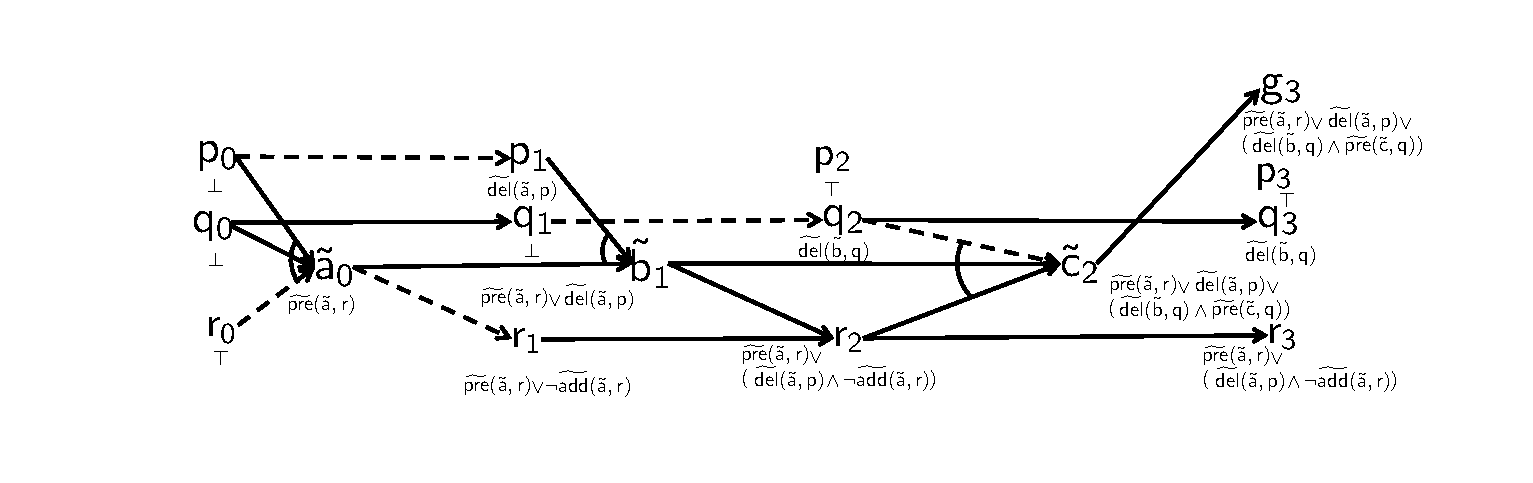
\includegraphics[width=.9\linewidth]{example.eps}
\vspace*{-1cm}\caption{\label{fig:example} Labeled Plan}
\end{figure*}


% the correctness of a plan by determining the incomplete features that can lead to plan failure, and counting the number of domain interpretations that succeed.
%Section \ref{sec:faults} describes how we measure the correctness of a plan in terms of the incompleteness and the following section discusses our choice of incomplete action representation in more detail.



%\section{Comparison of Possible Action Features with Local Closed Wolds}
%
%Definition \ref{def:incdomain} defines incomplete actions by sets of respective known and possible preconditions and effects.  GL define incomplete actions similar to STRIPS actions (Definition \ref{def:comact}) with additional local closed world statements of the form ${\tt DoesNotRelyOn}( \tilde{a}, p)$ ($p$ is not a precondition of $\tilde{a}$) or ${\tt CompletePreconditions}(\tilde{a})$  (the preconditions of $\tilde{a}$ are known).  
%
%We note that these representations are equivalent if we consider the set of known, possible, and impossible preconditions (and similarly for effects) of actions.  For example, ${\tt CompletePreconditions}(\tilde{a})$  is equivalent to stating $\widetilde{\tt pre}(\tilde{a}) = \{\}$ (i.e., the set of possible preconditions is empty).  Likewise, ${\tt DoesNotRelyOn}( \tilde{a}, p)$ is equivalent to stating $p \not\in \widetilde{\tt pre}(\tilde{a})$, and that for all $q \in P$ the lack of a statement ${\tt DoesNotRelyOn}(\tilde{a}, q)$ is equivalent to stating $q \in \widetilde{\tt pre}(\tilde{a})$ (i.e., impossible preconditions are not possible preconditions, and not impossible preconditions are possible preconditions).
%
%While the representations are equivalent, the obvious question is whether one is more succinct than the other.  The answer largely depends on the problem being modeled.  See Table \ref{tab:GLComparison} for examples.  Notice that the size of the representations is equivalent when stating, for example, that an action has complete preconditions; we either record the fact that the preconditions are complete or that the set of possible preconditions is empty.  The difference is with respect to stating, for example, that an individual proposition is not a precondition of an action.  Under our representation (Definition \ref{def:incact}), the set of possible preconditions would not contain a proposition, and under the GL representation it must be stated that the proposition is not a precondition.  However, if a proposition is a possible precondition to an action, we would record it as a possible precondition and GL would record nothing.  As such, the issue comes down to whether there are many possible or impossible preconditions and effects.  Our representation is smaller with many impossible features, and GL is smaller with many possible features.
%
%
%\begin{table}[h]
%\centering\begin{tabular}{|l|l|l|}
%\hline
% &Definition \ref{def:incact} & GL \\ \hline
% $\tilde{a}$ has only the known  & ${\tt pre}(\tilde{a}) = \{p, q\}$, & ${\tt pre}(\tilde{a}) = \{p, q\}$, \\ 
% preconditions $p, q$ & $\widetilde{\tt pre}(\tilde{a}) = \{\}$ & ${\tt CompletePreconditions}(\tilde{a})$\\ \hline
%$\tilde{a}$ has possible precondition $r$,  & ${\tt pre}(\tilde{a}) = \{\}$,  & ${\tt pre}(\tilde{a}) = \{\}$, \\
%but $z$ is neither a known nor a  & $\widetilde{\tt pre}(\tilde{a}) = \{r\}$ & ${\tt DoesNotRelyOn}( \tilde{a}, z)$ \\ 
%possible precondition & &  \\ \hline
%\end{tabular}
%\caption{\label{tab:GLComparison} Examples comparing representations.}
%\end{table}
%
%While we describe actions in the grounded (propositional) form, another practical concern is that we use PDDL \citep{pddl} action schemas to encode problems.  Under the GL representation, extending PDDL action schemas to state impossible preconditions (or effects) could require additional action schema parameters that refer to constants in predicates that are not preconditions.  If there are many impossible preconditions, then the action schemas could mention many additional parameters, which is known to lead to difficulty when grounding the schemas.  Our intuition is that possible action features are likely to share parameters with known action features and extending PDDL to support our representation will lead to fewer additional action schema parameters.  Furthermore, if there are many impossible features, our representation does not mention these features and therefore does not need to reference their parameters in the PDDL action schemas.  
%
%\section{Diagnosing Faults in Plans for Incomplete Domains}\label{sec:faults}
%
%An incomplete plan $\pi$ must achieve the goals under optimistic semantics (i.e., possible preconditions need not be satisfied, possible delete effects can be ignored, and possible add effects will occur), but we would prefer that plans succeed under more pessimistic conditions.  To quantify the extent to which our optimism is misleading, we introduce and expand upon GL's definitions of risks, which we refer to as faults.  A fault is a threat to the plan's causal proof that is introduced because of our optimism/ignorance of the underlying domain description.  For example, by assuming that possible delete effects do not occur, we introduce a fault when the possible delete effect does in fact delete a required subgoal.  By assuming the optimistic semantics, we allow plans that we would not otherwise consider, but by computing the faults we quantify the level to which the plan is susceptible to failure.  The challenge to computing faults is that incomplete action features may have a delayed impact on the plan or no impact at all, and we must determine if they are faults (i.e., guarantee plan failure if the incompleteness manifests unfavorably).
%
%Instead of reviewing GL's definitions, we take a new approach to develop the definitions of faults.  Our intuition is that plans with faults are best analyzed within the framework of model-based diagnosis \citep{reiter,dekleer}.  Among all of the techniques developed within model based diagnosis \citep{dekleer}, the most beneficial is a clear characterization of multiple-faults.  In contrast, GL discusses only single-faults, that they call risks, which do not explain plan failures that may occur because of multiple, interacting incomplete domain features.  For example, GL would consider a subgoal that is established by two different actions, which are subject to disjoint faults, as having no faults.  However, by using multiple-faults to explain failure to achieve the proposition, we see that the faults (at least one for each action) interact.   Clearly, single-faults are important for identifying a single-point-of-failure, but ignoring multiple-faults could lead to an overly optimistic assessment of a plan.  In the following, we generalize GL's notions of faults from singletons to sets, which we call diagnoses.  
%
% 
%%\noindent During plan synthesis we will not know which incomplete features are part of the ground-truth domain description, but we can determine which features, if manifested, are faults that invalidate the plan.  To compute these sets of faults, we turn to model based diagnosis.  A diagnosis is a hypothesis that a set of (co-occurring) faults explains failure in a system.  Multiple diagnoses (each containing multiple faults) may justify plan failure.
%
%\subsection{Model Based Diagnosis}  In defining the diagnoses of plan failure, we draw upon many well established techniques in model based diagnosis (MBD) \citep{reiter,dekleer}.  Viewing the plan as a physical system, faults are sets of potentially faulty components that describe anomalous behavior, such as an action not having its preconditions satisfied or a goal not being achieved.  
%
%There are two terms from MBD that enable us describe which sets of faults may cause plan failure.  The first term, a {\em conflict set} \citep{dekleer}, is a set of faults where if at least one of the faults occurs, it can explain the anomalous behavior.  A conflict set is inherently disjunctive because any non-empty subset of the conflict set can explain the failure, and it is not required that all components are faulty.  The second term, a {\em diagnosis}, is a set of system components where every component must be faulty to explain the behavior.  In contrast with a conflict set, a diagnosis is conjunctive -- every component in the diagnosis must be faulty.  However, there may be multiple diagnoses and each diagnosis is a hypothesis explaining failure.  Because of their respective disjunctive and conjunctive semantics, conflict sets and diagnoses can be expressed by the prime implicates and prime implicants of a propositional sentence capturing knowledge of the faulty system \citep{}.
%
%\citet{reiter} formulates MBD within a system that is defined by a system description ${\tt SD}$ and system components ${\tt COMP}$, taking the respective form of first-order sentences and a finite set of constants.  The system description includes a distinct unary predicate ${\tt AB}(\cdot)$ that indicates abnormal behavior on the part of a system component.  For example, the sentence ${\tt ANDG}(x) \wedge \neg {\tt AB}(x) \rightarrow {\tt out}(x) = {\tt and}({\tt in1}(x), {\tt in2}(x))$ indicates that an And-gate that is not abnormal will have its output equal to the logical and of its two inputs.  Along with the system description, {\tt OBS} is an observation of the system's behavior.  For example, {\tt OBS} may contain the facts ${\tt out}(and_1) = 0, {\tt in1}(and_1) = 1, {\tt in2}(and_1) = 1$, which is anomalous.
%
%\citet{reiter} defines approaches to finding conflict sets and diagnoses that rely on refutation proofs. Showing that ${\tt SD} \cup {\tt OBS} \cup \{\neg{\tt AB}(c_1), ..., \neg{\tt AB}(c_n)\}$ is inconsistent means that $c_1, ..., c_n$ functioning normally does not explain ${\tt OBS}$.  That is,  $\{c_1, ..., c_n\}$ is a conflict set, of which a subset is to blame for the observation and at least one of the conflict set components is faulty.  For example, ${\tt SD} \cup {\tt OBS} \cup \{\neg{\tt AB}(and_1)\}$ is inconsistent, and $\{and_1\}$ is a conflict set.  Reiter also shows that we can refine the conflict sets to include only those components that are mentioned in the refutation proof tree, so that if ${\tt SD} \cup {\tt OBS} \cup \{\neg{\tt AB}(c_1), ..., \neg{\tt AB}(c_n)\}$ is inconsistent, but only $\{\neg{\tt AB}(c_i), ..., \neg{\tt AB}(c_j)\} \subseteq \{\neg{\tt AB}(c_1), ..., \neg{\tt AB}(c_n)\}$ appear in the refutation proof, then $\{\neg{\tt AB}(c_i), ..., \neg{\tt AB}(c_j)\}$ is a conflict set that subsumes $\{\neg{\tt AB}(c_1), ..., \neg{\tt AB}(c_n)\}$.
%
%A generate-and-test approach is a possible, but naive, method to finding all conflict sets, and upon finding all conflict sets one can compute all diagnoses.  \citet{reiter} defines a diagnosis as a minimal hitting set on the collection of minimal conflict sets; a hitting set $x$ on a collection of sets $C$ is a set where for each set $c \in C$, $c \cap x \not= \{\}$.  A minimal hitting set $x$ is a set where no proper subset $x' \subset x$ is a hitting set.  In our small example, $\{and_1\}$ is the only conflict set, making $\{and_1\}$ the only diagnosis.  In a more complex scenario where the minimal conflict sets are $\{c_1, c_2\}$ and $\{c_1, c_3\}$, the diagnoses are $\{c_1\}$ and $\{c_2, c_3\}$.  
%
%\subsection{Diagnosing Plan Faults in Incomplete Domains} We describe a plan with a set of clauses ${\tt SD}(\pi)$ and introduce a hypothetical observation that the goal action cannot be executed, ${\tt OBS} = \neg \tilde{\sf a}_n$, to determine if a set of incomplete domain features is a conflict set.  
%
%Recall that a conflict set is a set of components, of which some subset must be behaving abnormally to explain an anomalous observation.  In diagnosing plan faults, a conflict set is comprised of incomplete domain features.  However, there exists an asymmetry among the types of incomplete domain features because the absence of a possible add effect in the true domain can cause failure, but the presence of a possible precondition or possible delete effect can cause plan failure.  As such, conflict sets (and diagnoses) refer to negative literals for possible add effects and positive literals for possible preconditions and delete effects.  
%
%In diagnosing plan faults, conflict sets and diagnoses are of the form 
%
%\noindent $\{\neg{\sf \widetilde{add}(\tilde{a}, p)}, ..., \neg{\sf \widetilde{add}(\tilde{a}', p')},{\sf \widetilde{pre}(\tilde{b}, q)}, ..., {\sf \widetilde{pre}(\tilde{b}', q')}, {\sf \widetilde{del}(\tilde{c}, r)}, ...,{\sf \widetilde{del}(\tilde{c}', r')} \}$, 
%
%\noindent indicating the absence of possible add effects or the presence of possible preconditions or delete effects causes plan faults.  Thus, following Reiter's approach, if 
%
%\noindent $ \tilde{\sf a}_{-1} \cup {\tt SD}(\pi) \cup \neg {\sf a}_n \cup \{{\sf \widetilde{add}(\tilde{a}, p)}, ...,{\sf \widetilde{add}(\tilde{a}', p')}, \neg{\sf \widetilde{pre}(\tilde{b}, q)}, ..., \neg{\sf \widetilde{pre}(\tilde{b}', q')}, \neg{\sf \widetilde{del}(\tilde{c}, r)}, ..., \neg{\sf \widetilde{del}(\tilde{c}', r')} \}$,
%
%\noindent is inconsistent, then  
%
%\noindent $\{\neg{\sf \widetilde{add}(\tilde{a}, p)}, ..., \neg{\sf \widetilde{add}(\tilde{a}', p')},{\sf \widetilde{pre}(\tilde{b}, q)}, ..., {\sf \widetilde{pre}(\tilde{b}', q')}, {\sf \widetilde{del}(\tilde{c}, r)}, ...,{\sf \widetilde{del}(\tilde{c}', r')} \}$
%
%\noindent or a subset of it is a conflict set.  
%
%We find it more convenient to formulate an equivalent inference task  
%
%\noindent $ \tilde{\sf a}_{-1} \cup {\tt SD}(\pi) \cup  \{{\sf \widetilde{add}(\tilde{a}, p)}, ...,{\sf \widetilde{add}(\tilde{a}', p')}, \neg{\sf \widetilde{pre}(\tilde{b}, q)}, ..., \neg{\sf \widetilde{pre}(\tilde{b}', q')}, \neg{\sf \widetilde{del}(\tilde{c}, r)}, ..., \neg{\sf \widetilde{del}(\tilde{c}', r')} \}\models {\sf a}_n$, 
%
%\noindent and use a theorem prover that is based on Modus Ponens and negation as failure.  In the following section, we make use of the intuitions developed in this section using Modus Ponens (we show that negation as failure can be made unnecessary) to motivate a forward-chaining state-space planner.  
%
%
%The system description ${\tt SD}(\pi)$ consists of clauses that define the semantics of plans in incomplete domains, which includes conditions under which an action will have its preconditions satisfied and its effects will change the current state.  This subsection i) presents the system description and maps it to the original definitions of plans for incomplete planning problems, ii) shows how the system description can be simplified without loss of generality, and iii) describes how an assumption-based truth maintenance system (ATMS) \cite{dekleer} can support more efficient diagnosis computation.  
%
%%We use two alternative system descriptions to diagnosing faults in plans in incomplete domains.  The first relies on a complete system description ${\tt SD}_C(\pi)$ that requires non-definite clauses, and the second, an incomplete system description ${\tt SD}_I(\pi)$ requires only definite clauses.  As we will show, reasoning with definite clauses provides a convenient way of computing the diagnoses with an assumption-based truth maintenance system (ATMS), where the assumptions do not require negated literals.  In the following, we discuss each formulation of the system description and follow with how an ATMS can be utilized with each.
%
%\begin{table}[t]
%\begin{tabular}{lrlll}
%%i)& ${\sf p_0}$ & &&for each $p \in I$\\
%%ii) &${\sf \tilde{a}_0}$&$\leftarrow$& $\left(\bigwedge\limits_{p \in {\tt pre}(\tilde{a}_0)} {\sf p_0}\right)\wedge$\\
%%&&& $\left(\bigwedge\limits_{p \in \widetilde{\tt pre}(\tilde{a}_0)} ({\sf p_0} \vee \neg{\tt OP}(\tilde{a}_0, p)) \right)$\\
%%x) &${\sf \tilde{a}_{t+1}}$& $\rightarrow$ & ${\sf \tilde{a}_{t}}\wedge\left( \bigwedge\limits_{p \in {\tt pre}(\tilde{a}_{t+1})} {\sf p_{t+1}}\right)\wedge$\\
%% &&& $\left(\bigwedge\limits_{p \in \widetilde{\tt pre}(\tilde{a}_{t+1})} ({\sf p_{t+1}} \vee \neg{\tt OP}(\tilde{a}_{t+1}, p))\right)  $& $t = -1... n-1$\\
%%x) &${\sf p_{t+1}} \wedge \neg {\sf p_{t}}$& $\rightarrow$ & ${\sf \tilde{a}_{t}}$& for all $p \in {\tt add}(\tilde{a}_t)$ \\
%%x) &${\sf p_{t+1}} \wedge \neg {\sf p_{t}}$& $\rightarrow$ & ${\sf \tilde{a}_{t}} \wedge {\tt UE}(\tilde{a}_t, p)$& for all $p \in \widetilde{\tt add}(\tilde{a}_t)$ \\
%%x) &$\neg {\sf p_{t+1}} \wedge {\sf p_{t}}$& $\rightarrow$ & ${\sf \tilde{a}_{t}}$& for all $p \in {\tt del}(\tilde{a}_t)$ \\
%%x) &$\neg {\sf p_{t+1}} \wedge {\sf p_{t}}$& $\rightarrow$ & ${\sf \tilde{a}_{t}} \wedge {\tt PC}(\tilde{a}_t, p)$& for all $p \in \widetilde{\tt del}(\tilde{a}_t)$ \\
%%
%%x) &${\sf \tilde{a}_{t+1}}$& $\rightarrow$ & ${\sf \tilde{a}_{t}}$& $t = -1... n-1$\\
%%x) &${\sf \tilde{a}_{t+1}}$& $\rightarrow$ & $ {\sf p_{t+1}}$ & for all $p \in {\tt pre}(\tilde{a}_{t+1}), t = -1... n-1$\\
%%x) &${\sf \tilde{a}_{t+1}}$& $\rightarrow$ & $ {\sf p_{t+1}} \vee \neg{\tt OP}(\tilde{a}_{t+1}, p)$ & for all $p \in\widetilde{\tt pre}(\tilde{a}_{t+1}), t = -1... n-1$\\
%%x) &${\sf p_{t+1}} \wedge \neg {\sf p_{t}}$& $\rightarrow$ & ${\sf \tilde{a}_{t}} \wedge {\tt UE}(\tilde{a}_t, p)$& for all $p \in \widetilde{\tt add}(\tilde{a}_t)$ \\
%%x) &$\neg {\sf p_{t+1}} \wedge {\sf p_{t}}$& $\rightarrow$ & ${\sf \tilde{a}_{t}}$& for all $p \in {\tt del}(\tilde{a}_t)$ \\
%%x) &$\neg {\sf p_{t+1}} \wedge {\sf p_{t}}$& $\rightarrow$ & ${\sf \tilde{a}_{t}} \wedge {\tt PC}(\tilde{a}_t, p)$& for all $p \in \widetilde{\tt del}(\tilde{a}_t)$ \\
%% \\
%% x) &$\neg {\sf \tilde{a}_{t+1}} \vee {\sf \tilde{a}_{t}}$& $t = -1... n-1$\\
%%x) &$\neg {\sf \tilde{a}_{t+1}}\vee {\sf p_{t+1}}$ & for all $p \in {\tt pre}(\tilde{a}_{t+1}), t = -1... n-1$\\
%%x) &$\neg {\sf \tilde{a}_{t+1}}\vee {\sf p_{t+1}} \vee \neg{\tt OP}(\tilde{a}_{t+1}, p)$ & for all $p \in\widetilde{\tt pre}(\tilde{a}_{t+1}), t = -1... n-1$\\
%%x) &$\neg {\sf p_{t+1}} \vee {\sf p_{t}}\vee {\sf \tilde{a}_{t}} $& for all $p \in \widetilde{\tt add}(\tilde{a}_t)$ \\
%%x) &$\neg {\sf p_{t+1}} \vee {\sf p_{t}}\vee {\tt UE}(\tilde{a}_t, p)$& for all $p \in \widetilde{\tt add}(\tilde{a}_t)$ \\
%%x) &${\sf p_{t+1}} \vee \neg {\sf p_{t}} \vee {\sf \tilde{a}_{t}}$& for all $p \in {\tt del}(\tilde{a}_t)$ \\
%%x) &${\sf p_{t+1}} \vee \neg {\sf p_{t}} \vee {\sf \tilde{a}_{t}}$& for all $p \in \widetilde{\tt del}(\tilde{a}_t)$ \\
%%x) &${\sf p_{t+1}} \vee \neg {\sf p_{t}} \vee {\tt PC}(\tilde{a}_t, p)$& for all $p \in \widetilde{\tt del}(\tilde{a}_t)$ \\
%% \\
%% x) &$\neg {\sf \tilde{a}_{t+1}} \leftarrow \neg {\sf \tilde{a}_{t}}$& $t = -1... n-1$\\
%%x) &$\neg {\sf \tilde{a}_{t+1}}\leftarrow \neg {\sf p_{t+1}}$ & for all $p \in {\tt pre}(\tilde{a}_{t+1}), t = -1... n-1$\\
%%x) &$\neg {\sf \tilde{a}_{t+1}}\leftarrow \neg {\sf p_{t+1}} \wedge {\tt OP}(\tilde{a}_{t+1}, p)$ & for all $p \in\widetilde{\tt pre}(\tilde{a}_{t+1}), t = -1... n-1$\\
%%x) &$\neg {\sf p_{t+1}} \leftarrow \neg {\sf p_{t}}\wedge \neg {\sf \tilde{a}_{t}} $& for all $p \in \widetilde{\tt add}(\tilde{a}_t)$ \\
%%x) &$\neg {\sf p_{t+1}} \leftarrow \neg {\sf p_{t}}\wedge \neg{\tt UE}(\tilde{a}_t, p)$& for all $p \in \widetilde{\tt add}(\tilde{a}_t)$ \\
%%x) &${\sf p_{t+1}} \leftarrow   {\sf p_{t}} \wedge \neg{\sf \tilde{a}_{t}}$& for all $p \in {\tt del}(\tilde{a}_t)$ \\
%%x) &${\sf p_{t+1}} \leftarrow  {\sf p_{t}} \wedge \neg {\sf \tilde{a}_{t}}$& for all $p \in \widetilde{\tt del}(\tilde{a}_t)$ \\
%%x) &${\sf p_{t+1}} \leftarrow {\sf p_{t}} \wedge \neg{\tt PC}(\tilde{a}_t, p)$& for all $p \in \widetilde{\tt del}(\tilde{a}_t)$ \\
% 
%i) & ${\sf \tilde{a}_{t+1}}$& $\leftarrow$ & ${\sf \tilde{a}_{t}}\wedge\left( \bigwedge\limits_{p \in {\tt pre}(\tilde{a}_{t+1})} {\sf p_{t+1}}\right)\wedge$\\
% &&& $\left(\bigwedge\limits_{p \in \widetilde{\tt pre}(\tilde{a}_{t+1})} ({\sf p_{t+1}} \vee \neg\widetilde{{\tt pre}}(\tilde{a}_{t+1}, p))\right)  $& $t = -1... n-1$\\
%ii) & ${\sf p_{t+1}}$ & $\leftarrow$ & ${\sf \tilde{a}_t}$& for all $p \in {\tt add}(\tilde{a}_t)$ \\
%% $a_t \rightarrow \neg p_{t+1}$, for all $p \in {\tt del}(\tilde{a})$ 
% iii) &${\sf p_{t+1}}$ & $\leftarrow$&${\sf \tilde{a}_t} \wedge \widetilde{{\tt add}}(\tilde{a}_t, p)$& for all $p \in \widetilde{\tt add}(\tilde{a}_t)$ \\
%iv) &${\sf p_{t+1}}$ & $\leftarrow$& ${\sf p_t}\wedge (\neg {\sf \tilde{a}_t} \vee  \neg\widetilde{{\tt del}}(\tilde{a}_t, p))$&  for all $p \in \widetilde{\tt del}(\tilde{a}_t)$\\
%v)  &$ {\sf p_{t+1}}$  & $\leftarrow$ & ${\sf p_t}$&  for all $p \in P\backslash({\tt del}(\tilde{a}_t) \cup \widetilde{\tt del}(\tilde{a}_t))$\\
%\end{tabular}
%\caption{\label{tab:csysdesc} The incomplete plan system description, ${\sf SD}(\pi)$.}
%\end{table}
%
%\und{Plan System Description} The system description  ${\tt SD}(\pi)$ is listed in Table \ref{tab:csysdesc}.   The clauses include conditions under which actions are successfully executed, and conditions under which a proposition will be true as a result of applying an action.  The clauses can be understood as stating: i)  actions require their preconditions to be satisfied {\em but also require the previous action to be successful}, ii) add effects are proven if the action is proven, iii) possible add effects are proven if the action is executed and the possible add effect is actually an add effect, iv) propositions that are possibly deleted will in fact be true if they were previously true and either the action fails or they are in fact not deleted, and v) all non-deleted propositions are true if they were previously true.
%
% The system description of the example plan $(\tilde{a}, \tilde{b}, \tilde{c})$ from Section \ref{sec:background} is as follows:
%% , where the incomplete features are represented by the shortened notation $\{{\sf f_0}, {\sf f_1}, {\sf f_2}, {\sf f_3}, {\sf f_4}\} = \{{\sf \widetilde{pre}(\tilde{a}, r)}, \widetilde{del}(\tilde{a}, p), \widetilde{add}(\tilde{a}, r), \widetilde{del}(\tilde{b}, q), \widetilde{pre}(\tilde{c}, q)\}$:
%
%
%\begin{tabular}{llll}
%\begin{minipage}{5cm}
%\begin{tabular}{l}
%%${\sf \tilde{a}_{-1}}$\\
%${\sf \tilde{a}_{-1}}\rightarrow {\sf p_0}$\\
%${\sf \tilde{a}_{-1}}\rightarrow  {\sf q_0}$\\
%${\sf \tilde{a}_{-1}} \wedge {\sf p_0}\wedge {\sf q_0}\wedge  {\sf r_0} \rightarrow {\sf \tilde{a}_0}$
%\\ ${\sf \tilde{a}_{-1}} \wedge {\sf p_0}\wedge {\sf q_0}\wedge \neg {\sf \widetilde{pre}(\tilde{a}, r)} \rightarrow {\sf \tilde{a}_0}$
%
%\\ $\neg {\sf \tilde{a}_0}\wedge  {\sf p_0} \rightarrow  {\sf p_1}$
%\\ ${\sf p_0}\wedge \neg {\sf \widetilde{del}(\tilde{a}, p)} \rightarrow  {\sf p_1}$
%
%\\ ${\sf \tilde{a}_0}\wedge {\sf \widetilde{add}(\tilde{a}, r)} \rightarrow  {\sf r_1}$
%\\ ${\sf q_0} \rightarrow  {\sf q_1}$
%\end{tabular}
%\end{minipage}
%&
%\begin{minipage}{4cm}
%\begin{tabular}{l}
%\\ ${\sf \tilde{a}_0}\wedge {\sf p_1} \rightarrow {\sf \tilde{b}_1}$
%
%\\ $\neg {\sf \tilde{b}_1}\wedge {\sf q_1} \rightarrow  {\sf q_2}$
%\\ $ {\sf q_1}\wedge \neg {\sf \widetilde{del}(\tilde{b}, q)} \rightarrow  {\sf q_2}$
%
%\\ ${\sf \tilde{b}_1} \rightarrow {\sf r_2}$
%\\ ${\sf r_1} \rightarrow {\sf r_2}$
%\\\\\\\\\\
%\end{tabular}
%\end{minipage}
%&
%\begin{minipage}{4cm}
%\begin{tabular}{l}
% ${\sf \tilde{b}_1}\wedge {\sf q_2}\wedge {\sf r_2} \rightarrow {\sf \tilde{c}_2}$
%\\ ${\sf \tilde{b}_1}\wedge \neg {\sf \widetilde{pre}(\tilde{c}, q)}\wedge {\sf r_2} \rightarrow {\sf \tilde{c}_2}$
%\\ ${\sf \tilde{c}_2} \rightarrow {\sf g_3}$
%\\ ${\sf q_2} \rightarrow  {\sf q_3}$
%\\ ${\sf r_2} \rightarrow {\sf r_3}$
%\\ ${\sf \tilde{c}_2} \wedge {\sf g_3} \rightarrow \tilde{\sf a}_3$
%\\\\\\\\
%\end{tabular}
%\end{minipage}
%\end{tabular}
%
%\noindent We note that the only non-definite clauses correspond to the cases where an action fails to execute and thus cannot possibly clobber the corresponding possibly deleted proposition (e.g., $\tilde{a}$ possibly deletes $p$, and we include the clause $\neg {\sf \tilde{a}_0}\wedge  {\sf p_0} \rightarrow  {\sf p_1}$).  As we will show, below we can simplify the system description to remove such clauses.  For all other clauses, we can create definite clauses by replacing each negated literal $\neg {\sf f_i}$ by a positive literal ${\sf nf_i}$.  
%
%
%We establish the correctness of the system description with the following theorem, that states that a plan is valid in an interpretation $D^i$ of an incomplete domain if and only if ${\sf a}_{-1} \cup {\tt SD}(\pi)  \cup {\sf F^i}$ entails ${\sf a}_n$, where 
%${\sf F^i} = 
%\{{\sf f} | f \in F^i\} \cup \{\neg {\sf f} | f \not\in F^i\}
%%\{\neg {\sf \widetilde{pre}(\tilde{a}, p)} |  \widetilde{pre}(\tilde{a}, r) \not\in F^i\} \cup 
%%\{        {\sf \widetilde{add}(\tilde{a}, p)} | \widetilde{add}(\tilde{a}, r)\in F^i\} \cup 
%%\{\neg {\sf \widetilde{del}(\tilde{a}, p)} |  \widetilde{del}(\tilde{a}, r)\not\in F^i\}
%$.
%
%\begin{theorem}  ${\sf a}_{-1} \cup {\tt SD}(\pi)  \cup {\sf F^i}  \models  {\sf a}_n$ iff $\pi$ is a plan in interpretation $D^i$.
%\end{theorem}
%\begin{proof}  We first show that ${\sf a}_{-1} \cup {\tt SD}(\pi)  \cup {\sf F^i}  \models  {\sf a}_n$ iff ${\sf a}_{-1} \cup {\tt SD}^i(\pi) \models  {\sf a}_n$, where ${\tt SD}^i(\pi)$ is the system description of a complete planning domain corresponding to interpretation $D^i$, and then that ${\sf a}_{-1} \cup {\tt SD}^i(\pi) \models  {\sf a}_n$ iff $\pi$ is a plan in interpretation $D^i$.
%
%${\tt SD}(\pi) \cup {\sf F^i}$ can be converted to conjunctive normal form, and, through unit propagation, each clause involving an incomplete domain literal will either become satisfied and removed or the literal will be removed from the clause because it cannot satisfy the clause.  The resulting set of clauses does not include any incomplete domain literals in ${\sf F^i}$, and is equivalent to the system description ${\tt SD}^i(\pi)$ of the incomplete domain interpretation $D^i$, defined as follows: 
%
%\begin{tabular}{lrlll}
%i)& ${\sf \tilde{a}_{t+1}}$& $\leftarrow$ & ${\sf \tilde{a}_{t}}\wedge \bigwedge\limits_{p \in {\tt pre}(a^i_{t+1})} {\sf p_{t+1}}  $& $t = -1... n-1$\\
%ii)& ${\sf p_{t+1}}$ & $\leftarrow$ & ${\sf \tilde{a}_t}$& for all $p \in {\tt add}(a^i_t)$ \\
%iii) &${\sf p_{t+1}}$ & $\leftarrow$& ${\sf p_t}\wedge \neg {\sf \tilde{a}_t}$&  for all $p \in {\tt del}(a^i_t)$\\
%v)  &$ {\sf p_{t+1}}$  & $\leftarrow$ & ${\sf p_t}$&  for all $p \in P\backslash {\tt del}(a^i_t)$\\
%\end{tabular}
%
%It is clear that ${\sf a}_{-1} \cup {\tt SD}^i(\pi) \models  {\sf a}_n$ iff  $\pi$ is a valid plan in interpretation $D^i$ because i) the plan is valid only if each action has its preconditions satisfied, ii) the successor state at time $t+1$ must include the add effects of the action applied at time $t$, iii) the successor state will only include a deleted proposition if the applied action fails (but no valid plan allows action failures), and iv) propositions that are not deleted will be true in the successor state. 
%
%Therefore, by simplifying the incomplete plan system description ${\tt SD}(\pi) \cup {\sf F^i}$ to the complete plan system description ${\tt SD}^i(\pi)$ for an domain interpretation $D^i$, and showing its correspondence to the plan semantics of a plan in a domain interpretation, ${\sf a}_{-1} \cup {\tt SD}(\pi)  \cup {\sf F^i}  \models  {\sf a}_n$ iff $\pi$ is a plan in interpretation $D^i$.
%\end{proof}
%
%Simplifying the system description for the domain interpretation where $F^0
% = \{\widetilde{add}(\tilde{a}, r), \widetilde{pre}(\tilde{c}, q)\}$, we obtain ${\tt SD}^0(\pi)$:
%
%
%\begin{tabular}{llll}
%\begin{minipage}{4cm}
%\begin{tabular}{l}
%%${\sf \tilde{a}_{-1}}$\\
%${\sf \tilde{a}_{-1}}\rightarrow {\sf p_0}$\\
%${\sf \tilde{a}_{-1}}\rightarrow  {\sf q_0}$\\
%${\sf \tilde{a}_{-1}} \wedge {\sf p_0}\wedge {\sf q_0}\wedge  {\sf r_0} \rightarrow {\sf \tilde{a}_0}$
%\\ ${\sf \tilde{a}_{-1}} \wedge {\sf p_0}\wedge {\sf q_0} \rightarrow {\sf \tilde{a}_0}$
%
%\\ $\neg {\sf \tilde{a}_0}\wedge  {\sf p_0} \rightarrow  {\sf p_1}$
%\\ ${\sf p_0} \rightarrow  {\sf p_1}$
%
%\\ ${\sf \tilde{a}_0} \rightarrow  {\sf r_1}$
%\\ ${\sf q_0} \rightarrow  {\sf q_1}$
%\end{tabular}
%\end{minipage}
%&
%\begin{minipage}{4cm}
%\begin{tabular}{l}
%\\ ${\sf \tilde{a}_0}\wedge {\sf p_1} \rightarrow {\sf \tilde{b}_1}$
%
%\\ $\neg {\sf \tilde{b}_1}\wedge {\sf q_1} \rightarrow  {\sf q_2}$
%\\ $ {\sf q_1} \rightarrow  {\sf q_2}$
%
%\\ ${\sf \tilde{b}_1} \rightarrow {\sf r_2}$
%\\ ${\sf r_1} \rightarrow {\sf r_2}$
%\\\\\\\\\\
%\end{tabular}
%\end{minipage}
%&
%\begin{minipage}{4cm}
%\begin{tabular}{l}
% ${\sf \tilde{b}_1}\wedge {\sf q_2}\wedge {\sf r_2} \rightarrow {\sf \tilde{c}_2}$
%\\ ${\sf \tilde{c}_2} \rightarrow {\sf g_3}$
%\\ ${\sf q_2} \rightarrow  {\sf q_3}$
%\\ ${\sf r_2} \rightarrow {\sf r_3}$
%\\ ${\sf \tilde{c}_2} \wedge {\sf g_3} \rightarrow \tilde{\sf a}_3$
%\\\\\\\\
%\end{tabular}
%\end{minipage}
%\end{tabular}
%
%Upon inspection, it is possible to see that $\tilde{\sf a}_{-1} \cup {\tt SD}^i(\pi)\models  \tilde{\sf a}_3$.
%
%%However, because some of the action literals appear in both the positive and negative, we cannot substitute new literals, as is the case with the fault literals.  
%
%If we find examine all subsets of the incomplete features ${\cal F}$, for example $\{\widetilde{pre}(\tilde{a}, r),  \widetilde{del}(\tilde{a}, p), \widetilde{add}(\tilde{a}, r), \widetilde{del}(\tilde{b}, q), \widetilde{pre}(\tilde{c}, q)\}$, where $\tilde{\sf a}_{-1} \cup {\tt SD}(\pi) \cup  \{\neg{\sf \widetilde{pre}(\tilde{a}, r)}, \neg{\sf \widetilde{del}(\tilde{a}, p)}, {\sf \widetilde{add}(\tilde{a}, r)}, \neg{\sf \widetilde{del}(\tilde{b}, q)}, \neg{\sf \widetilde{pre}(\tilde{c}, q)}\} \models \tilde{\sf a}_3$, then we can determine the minimal conflict sets. In our example, we can derive the following minimal conflict sets:
%
%$\{ \widetilde{pre}(\tilde{a}, r), \widetilde{del}(\tilde{a}, p), \widetilde{del}(\tilde{b}, q)\}$
%
%$\{ \widetilde{pre}(\tilde{a}, r), \widetilde{del}(\tilde{a}, p), \widetilde{pre}(\tilde{c}, q)\}$
%
%\noindent From the conflict sets, we determine the following diagnoses:
%
%$\{\widetilde{pre}(\tilde{a}, r)\}$
%
%$\{\widetilde{del}(\tilde{a}, p)\}$
%
%$\{\widetilde{del}(\tilde{b}, q), \widetilde{pre}(\tilde{c}, q)\}$
%
%The diagnoses are cases that will guarantee plan failure.  If the first action $\tilde{a}$ can fail because of an open precondition fault.  The second action $\tilde{b}$ can fail because its precondition $p$ is deleted by $\tilde{a}$ due to a possible clobberer fault.  The third action $\tilde{c}$ can fail if its possible precondition $q$ is required (an open precondition fault) and the second action $\tilde{b}$ possibly deletes $q$ (a possible clobberer fault).
%
%\und{Simplified System Description}  The system description is complicated by the fact that we must seemingly account for faults that result because an action fails and cannot possibly clobber a proposition or the action does not fail and possibly clobbers the proposition (cf. rule iv) in Table \ref{tab:csysdesc}).  Rewriting this rule results in the following two clauses:
%
%${\sf p_{t+1}}\leftarrow{\sf p_t}\wedge \neg {\sf \tilde{a}_t} $
%
%${\sf p_{t+1}}\leftarrow{\sf p_t}\wedge  \neg{\tt PC}(\tilde{a}_t, p)$
%
%\noindent of which only the second can be made into a definite clause.  The issue is whether we can make the same inferences with and without the first of the two clauses above because, without the first, the theorem prover can be based solely upon modus ponens and simplify our use of an ATMS in the next section.  
%
%We define ${\tt SD}'(\pi)$ by replacing rule iv) in Table \ref{tab:csysdesc} by the rule:
%${\sf p_{t+1}} \leftarrow {\sf p_t}\wedge  \neg{\tt PC}(\tilde{a}_t, p) $  for all $p \in \widetilde{\tt del}(\tilde{a}_t)$.  To show that the same set of diagnoses can be computed with either system description, we establish the following theorem.
%
%
%
%\begin{theorem} ${\sf a}_{-1} \cup {\tt SD}(\pi)  \cup {\sf F} \models  {\sf a}_n$  iff ${\sf a}_{-1} \cup {\tt SD}'(\pi)\cup {\sf F} \models  {\sf a}_n$, where ${\sf F}$ is a set of literals denoting incomplete features.
%\end{theorem}
%\begin{proof}
%The clauses defined by ${\tt SD}'(\pi)$ are a subset of the clauses defined by ${\tt SD}(\pi)$, making any proof using ${\tt SD}'(\pi)$ also possible with ${\tt SD}(\pi)$; therefore if ${\sf a}_{-1} \cup {\tt SD}'(\pi)  \cup{\sf F}\models {\sf a}_n  $ then ${\sf a}_{-1} \cup {\tt SD}(\pi)  \cup{\sf F} \models {\sf a}_n $.
%
%To show the converse, we show that no proof involves ${\sf p_{t+1}}\leftarrow{\sf p_t}\wedge \neg {\sf \tilde{a}_t}  \in {\tt SD}(\pi)$.  If we can derive  $\neg {\sf \tilde{a}_t}$ by negation as failure, then by induction on rule i), we cannot derive ${\sf a}_n$.  Therefore, if ${\sf a}_{-1} \cup {\tt SD}(\pi)  \cup{\sf F} \models {\sf a}_n$ then ${\sf a}_{-1} \cup {\tt SD}'(\pi)  \cup{\sf F} \models {\sf a}_n$.
%\end{proof}
%
%%\und{Incomplete Plan System Description}  The incomplete system description ${\tt SD}_I(\pi)$  of a plan $\pi = (\tilde{a}_0, ..., \tilde{a}_{n-1})$ is identical to the complete system description, except that we replace rule vi) in Table \ref{tab:csysdesc} by the following rule:
%%
%%${\sf p_t}\wedge \neg{\tt PC}(\tilde{a}_t, p)\rightarrow  {\sf p_{t+1}}$   for all $p \in \widetilde{\tt del}(\tilde{a}_t)$
%%
%%\noindent The significance of this new rule is that we can describe the plan by definite clauses at the expense of ignoring potential future faults introduced by the action failing to execute (focussing only on the faults introduced by the action succeeding).  
%%
%%For example, under the incomplete system description, the following set of clauses describes our example plan $(\tilde{a}, \tilde{b}, \tilde{c})$, where again the faults are denoted by the shortened notation where $\{{\sf f_0}, {\sf f_1}, {\sf f_2}, {\sf f_3}, {\sf f_4}\} = \{{\tt OP}(\tilde{a}, r), {\tt PC}(\tilde{a}, p), {\tt UE}(\tilde{a}, r), {\tt PC}(\tilde{b}, q), {\tt OP}(\tilde{c}, q)\}$:
%%
%%\begin{tabular}{llll}
%%\begin{minipage}{4cm}
%%\begin{tabular}{l}
%%%$\neg {\sf f_0}$, $\neg {\sf f_1}$, $\neg {\sf f_2}$, $\neg {\sf f_3}$,  $\neg {\sf f_4}$
%%${\sf p_0}$\\  ${\sf q_0}$\\
%%%\\\\\\\\
%%%\end{tabular}
%%%\end{minipage}
%%%&
%%%\begin{minipage}{3cm}
%%%\begin{tabular}{l}
%%${\sf p_0}, {\sf q_0}, {\sf r_0} \rightarrow {\sf \tilde{a}_0}$
%%\\ ${\sf p_0}, {\sf q_0}, \neg {\sf f_0} \rightarrow {\sf \tilde{a}_0}$
%%\\ ${\sf p_0}, \neg {\sf f_1} \rightarrow  {\sf p_1}$
%%\\ ${\sf \tilde{a}_0}, \neg {\sf f_2} \rightarrow  {\sf r_1}$
%%\\ ${\sf q_0} \rightarrow  {\sf q_1}$
%%\end{tabular}
%%\end{minipage}
%%&
%%\begin{minipage}{3cm}
%%\begin{tabular}{l}
%% ${\sf \tilde{a}_0}, {\sf p_1} \rightarrow {\sf \tilde{b}_1}$
%%\\ $ {\sf q_1}, \neg {\sf f_3} \rightarrow  {\sf q_2}$
%%\\ ${\sf \tilde{b}_1} \rightarrow {\sf r_2}$
%%\\ ${\sf r_1} \rightarrow {\sf r_2}$
%%\\\\\\
%%\end{tabular}
%%\end{minipage}
%%&
%%\begin{minipage}{3cm}
%%\begin{tabular}{l}
%% ${\sf \tilde{b}_1}, {\sf q_2}, {\sf r_2} \rightarrow {\sf \tilde{c}_2}$
%%\\ ${\sf \tilde{b}_1}, \neg {\sf f_4}, {\sf r_2} \rightarrow {\sf \tilde{c}_2}$
%%\\ ${\sf \tilde{c}_2} \rightarrow {\sf g_3}$
%%\\ ${\sf q_2} \rightarrow  {\sf q_3}$
%%\\ ${\sf r_2} \rightarrow {\sf r_3}$\\\\
%%\end{tabular}
%%\end{minipage}
%%\end{tabular}
%%
%%\noindent Again, we can replace the negated fault literals by corresponding positive literals to attain definite clauses.
%
%
%
%
%
%
%%\begin{figure}
%%\centering
%%\includegraphics[width=.75\columnwidth]{plangraphhobddc.eps}
%%\caption{\label{fig:plangraphhobddc} Assumptions in complete system description for plan $(\tilde{a}, \tilde{b}, \tilde{c})$.}
%%\end{figure}
%
%\begin{figure}
%\centering
%\includegraphics[width=\columnwidth]{plangraphhobdd1.eps}
%\caption{\label{fig:plangraphhcs} Fault labels and proof trees for the system description of plan $(\tilde{a}, \tilde{b}, \tilde{c})$.}
%\end{figure}
%
%
%Figure \ref{fig:plangraphhcs} depicts several proof trees for the query
%${\sf a}_{-1} \cup {\tt SD}'(\pi) \cup \{\neg{\sf \widetilde{pre}(\tilde{a}, r)}, \neg{\sf \widetilde{del}(\tilde{a}, p)}, {\sf \widetilde{add}(\tilde{a}, r)}, \neg{\sf \widetilde{del}(\tilde{b}, q)}, \neg{\sf \widetilde{pre}(\tilde{c}, q)}\} \models {\sf a}_3$.  In the figure, the nodes represent the literals used in the query, and the directed hyper-edges denote clauses (edges connected by a curved arc denote a conjunction of the antecedents).   The propositional sentence annotations can be safely ignored until we discuss the use of the ATMS below.  The figure depicts multiple proofs -- ${\sf r_2}$ and ${\sf \tilde{c}_2}$ are both proven by two clauses, making a total of four distinct proofs.  Each proof relies on a different set of faults not being present; therefore, if any subset of the faults materializes, the proof will fail -- these sets of faults correspond to the conflict sets: 
%
%$\{ \widetilde{pre}(\tilde{a}, r), \widetilde{del}(\tilde{a}, p), \widetilde{del}(\tilde{b}, q)\}$
%
%$\{ \widetilde{pre}(\tilde{a}, r), \widetilde{del}(\tilde{a}, p), \widetilde{pre}(\tilde{c}, q)\}$
%
%$\{ \widetilde{pre}(\tilde{a}, r), \widetilde{del}(\tilde{a}, p), \neg \widetilde{add}(\tilde{a}, r), \widetilde{del}(\tilde{b}, q)\}$
%
%$\{ \widetilde{pre}(\tilde{a}, r), \widetilde{del}(\tilde{a}, p), \neg \widetilde{add}(\tilde{a}, r), \widetilde{pre}(\tilde{c}, q)\}$
%
%
%\noindent however, the last two conflict sets are not minimal because they are subsumed by one of the other conflict sets.  The minimal conflict sets are:
%
%$\{ \widetilde{pre}(\tilde{a}, r), \widetilde{del}(\tilde{a}, p), \widetilde{del}(\tilde{b}, q)\}$
%
%$\{ \widetilde{pre}(\tilde{a}, r), \widetilde{del}(\tilde{a}, p), \widetilde{pre}(\tilde{c}, q)\}$
%
%\noindent which allows us to compute the  following diagnoses (minimal hitting sets):
%
%
%$\{\widetilde{pre}(\tilde{a}, r)\}$
%
%$\{\widetilde{del}(\tilde{a}, p)\}$
%
%$\{\widetilde{del}(\tilde{b}, q), \widetilde{pre}(\tilde{c}, q)\}$
%
%
%\und{Truth Maintenance Systems} The generate-and-test method of computing conflict sets involves selecting all possible sets of literals ${\sf F}$ denoting incomplete features and determining if ${\sf a}_{-1} \cup {\tt SD}'(\pi)  \cup {\sf F} \models  {\sf a}_n$.  An alternative is to employ an assumption-based truth maintenance system (ATMS) \cite{atms} so that we can simultaneously compute all possible proofs for all possible sets ${\sf F}$.  The approach is to record a label for each literal that is proven to denote a set of contexts relevant to that literal.  In our scenario the contexts denote sets of incomplete domain features ${\sf F}$ that will prevent the proof of a literal.  
%%While it is possible to define labels so that they denote conflict sets (from which we can compute the diagnoses), we define the labels so that they natively represent the diagnoses.
%% each label refers to a set of diagnoses affecting a literal.  That is, instead of recording what is required to prove a literal in the label, we record what is required to prevent the proof of a literal.
%%We explore two approaches for representing the label; the first represents it by an OBDD, and the second represents it by a set of prime implicants (non-subsumed conjunctive clauses).  Both representations capture a set of propositional models that correspond to interpretations of the incomplete domain features.  
%%
%%There are many important differences between the representations that include, their size, the cost of model counting, and the cost of conjunction and disjunction.  The OBDD representation can be exponential-sized in the number of incomplete features, but permits polynomial-time model counting and conjunction/disjunction.  Prime implicants are not necessarily more succinct than OBDDs, require exponential-time model counting, and admit only polynomial-time conjunction \citep{adnan}.  Despite the seeming disadvantage of prime implicants, we note that they have an important structural property that we will use to our advantage -- we can count the number of prime implicants in time linear in the representation of the prime implicants.  Another important distinction is that, empirically, diagnoses tend to have a compact representation with prime implicants, especially under the incomplete system description.  As we will show, the diagnoses represented as prime implicants in the incomplete system require only positive literals.
%In the following, we present the definitions of the labels independent of any particular representation, but 
%%, with the understanding that a choice of representation will require different operations (ITE-operators in OBDDs or distributing conjunction and disjunction and removing subsumed implicates in prime implicates) to bring the propositional sentence into a normal form.  
%we describe the implementation of operations required for two alternative representations (prime implicants or OBDDs) in Section \ref{sec:empirical}.  
%%We present the definitions for labels both in the complete and incomplete system descriptions.
%
%To represent and compute the contexts preventing the proof of each literal, we recall that each diagnosis is a conjunction of literals
%
%\noindent $\{\neg {\sf \widetilde{add}(\tilde{a}, p)}, ..., \neg {\sf \widetilde{add}(\tilde{a}', p')},{\sf \widetilde{pre}(\tilde{b}, q)}, ...,{\sf \widetilde{pre}(\tilde{b}', q')},{\sf \widetilde{del}(\tilde{c}, r)}, ...,{\sf \widetilde{del}(\tilde{c}', r')} \}$
%
%\noindent where every conjunct must be true in order to cause failure.  As such, a label denoting diagnoses can be represented as a disjunction of diagnoses.  In the ATMS, we must label each possible premise with the diagnoses preventing its derivation. The possible premises include the initial action ${\sf a}_{-1}$, and elements from the set
%
%\noindent $\{{\sf \widetilde{add}(\tilde{a}, p)}, ..., {\sf \widetilde{add}(\tilde{a}', p')}, \neg{\sf \widetilde{pre}(\tilde{b}, q)}, ..., \neg{\sf \widetilde{pre}(\tilde{b}', q')}, \neg{\sf \widetilde{del}(\tilde{c}, r)}, ..., \neg{\sf \widetilde{del}(\tilde{c}', r')} \}$
%
%\noindent and the labels are defined
%
%\noindent $l({\sf a}_{-1}) = \perp$
%
%\noindent$l({\sf \widetilde{add}(\tilde{a}, p)}) = \neg {\sf \widetilde{add}(\tilde{a}, p)}$
%...
%$l({\sf \widetilde{add}(\tilde{a}', p')}) = \neg {\sf \widetilde{add}(\tilde{a}', p')}$
%
%\noindent$l(\neg {\sf \widetilde{pre}(\tilde{b}, q)}) = {\sf \widetilde{pre}(\tilde{b}, q)}$
% ...
%$l(\neg {\sf \widetilde{pre}(\tilde{b}', q')}) = {\sf \widetilde{pre}(\tilde{b}', q')}$
%
%\noindent$l(\neg {\sf \widetilde{del}(\tilde{c}, r)}) = {\sf \widetilde{del}(\tilde{c}, r)}$
% ...
%$l(\neg {\sf \widetilde{del}(\tilde{c}', r')}) = {\sf \widetilde{del}(\tilde{c}', r')}$
%
%\noindent The label of the initial action is $\perp$ (logical false) to denote that there is no diagnosis under which the initial action cannot be derived.  The label of each literal denoting an incomplete domain feature is the negation of the literal to denote that the only diagnosis under which the literal is not proven is when the literal is not true initially.  
%%With label propagation rules, the labels of the premises are combined to denote the diagnoses for derived literals.
%
%%An ATMS supports the computation of all proofs for all sets of premises by simultaneously asserting each possible premise ${\sf p}$ and labeling each $l({\sf p})$ to indicate the contexts in which it can be assumed.  As inferences are made, the ATMS combines the labels of literals used to derive a new literal to indicate which sets of premises will allow the proof of the new literal.  As previously stated, we invert the semantics of labels to denote which premises will prevent the deriving a literal.  The premises include literals of the form
%%
%%$\{{\sf \widetilde{add}(\tilde{a}, p)}, ..., {\sf \widetilde{add}(\tilde{a}', p')}, \neg{\sf \widetilde{pre}(\tilde{b}, q)}, ..., \neg{\sf \widetilde{pre}(\tilde{b}', q')}, \neg{\sf \widetilde{del}(\tilde{c}, r)}, ..., \neg{\sf \widetilde{del}(\tilde{c}', r')} \}$
%%
%%\noindent which may or may not hold in all contexts.  The premise ${\sf a}_{-1}$ will hold in all contexts, so we do not include it in any labels.
%
%
%
%%Each premise ${\sf p}$ (initial state literal) is associated with $l({\sf p}) = \perp$, indicating that under no interpretations will ${\sf p}$ be false.  For all fault literals $\neg{\sf f_i}$, we associate $l(\neg{\sf f_i}) = {\sf f_i}$ to denote that a fault being present will disprove that that it is not present.  
%
%All other literals are proven by one or more clauses, and we associate with each clause $h: {\sf q_1}, ..., {\sf q_m} \rightarrow {\sf p}$ that proves ${\sf p}$ a sentence $l(h, {\sf p}) = l({\sf q_1}) \vee ... \vee l({\sf q_m})$
%\noindent to denote that the clause will fail to prove ${\sf p}$ in any case where at least {\em one of} (hence the disjunction) its antecedents is not proven. 
%%If the clause includes a negated literal $\neg {\sf q_i}$ in the antecedent, as with the action literals in the complete system description, we replace $l(\neg {\sf q_i})$ with $\neg l({\sf q_i})$ when computing $l(h, {\sf p})$ above.  The intuition is that if the label $l({\sf q_i})$ represents the cases where we fail to prove ${\sf q_i}$, then because of the negation as failure (closed-world) semantics, we can conclude that $\neg l({\sf q_i})$ denotes the cases where we fail to prove $\neg {\sf q_i}$.
%Multiple clauses $h_1, ..., h_k$ may prove ${\sf p}$, allowing us to define 
%$l({\sf p}) = l(h_1, {\sf p}) \wedge ... \wedge l(h_k, {\sf p})$
%\noindent denoting that ${\sf p}$ will be unproven if {\em all of} (hence the conjunction) the clauses fail to prove ${\sf p}$.
%
%%$l({\sf a}_n)$ is a propositional sentence whose models are conjunctions of faults that will fail to achieve the goal because of plan failure.  Therefore if a propositional sentence $\phi$ over fault propositions fails to propositionally entail $l({\sf a}_n)$, all models of $\phi$ refer to domain interpretations under which a plan will fail.
%
%\begin{theorem}
%%if a conjunction of faults is not a model of the goal label, then no proof will require they be false.
%%If a proof requires the faults be false, then that conjunction of faults entails the goal label.
% $({\sf f_i} \wedge ... \wedge {\sf f_j})$ is a prime implicant of  $l({\sf p})$  iff  $\{{\sf f_i}, ..., {\sf f_j}\}$ is a diagnosis for ${\sf p}$.
%%Every  
%%${\sf a}_{-1} \cup {\tt SD}(\pi)  \cup \{\neg{\sf f_i}, ..., \neg{\sf f_j}\} \not\models  {\sf a}_n$  iff 
%%${\sf f_i} \vee ... \vee {\sf f_j} \not\models l({\sf a}_n) $
%\end{theorem}
%\begin{proof} 
%If $({\sf f_i} \wedge ... \wedge {\sf f_j})$ is a prime implicant of  $l({\sf p})$  then  $\{{\sf f_i}, ..., {\sf f_j}\}$ is a diagnosis for ${\sf p}$ because by the rules for defining $l({\sf p})$, each conjunct of the prime implicant is required to prevent a proof of ${\sf p}$ through some set of clauses, and asserting each literal in the diagnosis as a premise will prevent all proofs of ${\sf p}$, making it a diagnosis.
%
%If  $\{{\sf f_i}, ..., {\sf f_j}\}$ is a diagnosis for ${\sf p}$ then $({\sf f_i} \wedge ... \wedge {\sf f_j})$ is a prime implicant of  $l({\sf p})$  because assuming the diagnosis literals as premises will prevent any proof of ${\sf p}$, which means that under the label definitions all proofs of ${\sf p}$ must contribute at least one conjunct to the prime implicant.
%\end{proof}
%
%Figure \ref{fig:plangraphhcs} depicts the labels associated with each literal by the propositional sentence underneath the literal. 
%%Consider the complete system description assumption  $l({\sf p_1})$ in  Figure \ref{fig:plangraphhobddc}, that is computed in terms rules $h_1: {\sf \neg f_1} \wedge {\sf p_0} \rightarrow {\sf p_1}$ and $h_2: \neg{\sf \tilde{a}_0} \wedge {\sf p_0} \rightarrow {\sf p_1}$ and the following antecedent labels:
%%
%%$l({\sf \neg f_1}) = {\sf f_1}$
%%
%%$l({\sf p_0}) = \perp$
%%
%%$l({\sf \tilde{a}_0}) = {\sf f_0}$
%%
%%\noindent so that 
%%
%%$l(h_1, {\sf p_1}) = l({\sf nf_1}) \vee l({\sf p_0}) = {\sf f_1}$
%%
%%$l(h_2, {\sf p_1}) = l(\neg {\sf \tilde{a}_0}) \vee l({\sf p_0}) = \neg l( {\sf \tilde{a}_0}) \vee l({\sf p_0}) = \neg {\sf f_0}$
%%
%%\noindent and the label is defined
%%
%%$l({\sf p_1}) =  \neg {\sf f_0} \wedge {\sf f_1}$
%%
%Consider the incomplete system label $l({\sf \tilde{c}_2})$, that is proven by two clauses,  $h_3: {\sf \tilde{b}_1}, {\sf q_2}, {\sf r_2} \rightarrow {\sf \tilde{c}_2}$ and $h_4: {\sf \tilde{b}_1}, \neg{\sf f_4}, {\sf r_2} \rightarrow {\sf \tilde{c}_2}$.
%The label for each of the antecedents of the clauses are as follows:
%
%$l({\sf \tilde{b}_1}) = {\sf f_0} \vee {\sf f_1} $
%
%$l({\sf q_2}) = {\sf f_3}$
%
%$l({\sf r_2}) = {\sf f_0} \vee ({\sf f_1} \wedge {\sf f_2})$
%
%$l(\neg {\sf f_4}) = {\sf f_4}$
%
%\noindent allowing us to compute for each clause
%
%$l(h_3, {\sf \tilde{c}_2}) = l({\sf \tilde{b}_1}) \vee l({\sf q_2}) \vee l({\sf r_2}) = ({\sf f_0} \vee {\sf f_1}) \vee ({\sf f_3}) \vee ({\sf f_0} \vee ({\sf f_1} \wedge {\sf f_2})) = {\sf f_0} \vee {\sf f_1} \vee {\sf f_3} $
%
%$l(h_4, {\sf \tilde{c}_2}) = l({\sf \tilde{b}_1})  \vee l(\neg {\sf f_4}) \vee l({\sf r_2})= ({\sf f_0} \vee {\sf f_1})  \vee ({\sf f_4}) \vee ({\sf f_0} \vee ({\sf f_1} \wedge {\sf f_2})) =  {\sf f_0} \vee {\sf f_1}\vee {\sf f_4} $
%
%\noindent and define
%
%$l({\sf \tilde{c}_2}) = l(h_3, {\sf \tilde{c}_2}) \wedge l(h_4, {\sf \tilde{c}_2}) = ({\sf f_0} \vee {\sf f_1} \vee {\sf f_3}) \wedge ({\sf f_0} \vee {\sf f_1}\vee {\sf f_4}) = {\sf f_0} \vee {\sf f_1} \vee ({\sf f_3} \wedge {\sf f_4})$
%
%By counting the models of the label $l({\sf g_3})$, of the goal,  it is possible to determine how many interpretations of the incomplete domain will fail to achieve the goal with the plan.  In this example, there are thirty-two interpretations, and twenty-six will fail to achieve the goal.
%
%
%
%
%\subsection{Counting Models and Diagnoses}
%
%The labels computed in the previous section identify those combinations of incomplete domain features that can prohibit a plan from satisfying the goals (i.e., the models of the labels are interpretations of the incomplete domain that will fail).  From the labels, it is possible  to compute exactly how many interpretations of the incomplete domain features lead to a successful or unsuccessful plan.  Thus, counting the number of domains that will not successfully achieve the goals can be reduced to counting the models of the goal action label $l(\tilde{a}_n)$ (a propositional sentence).   The planner described in the next section is based on the idea of using an ATMS to represent plans,  and many of its subroutines involve comparing propositional sentences. In comparing a propositional sentence $\phi$ with another, we will refer to its set of models $M(\phi)$, its set of prime implicants $PI(\phi)$, and its set of $k$-element prime implicants $PI_k(\phi)$.
%
%While counting models requires polynomial time when a propositional sentence is represented by an OBDD, it requires exponential time when represented by prime implicants.   However, we note that the number of prime implicants can be indicative of the number of models, and simply counting the number of prime implicants can provide a heuristic measure.  
%
%From the example in the previous section, the three prime implicants  ${\sf f_0}\vee {\sf f_1}\vee ({\sf f_3} \wedge {\sf f_4})$ have twenty-six models, whereas the two prime implicants  ${\sf f_0} \vee {\sf f_1}$ have twenty-four models  -- the number of prime implicants, in this case, is proportional to the number of models.  While the relationship between prime implicants and models does not hold in general, we can use the number of prime implicants to heuristically compare propositional sentences (estimating the number of models).  
%
%Another observation is that having fewer prime implicants of smaller cardinality can result in fewer models.  For example, both ${\sf f_0}\vee{\sf f_1}$ and ${\sf f_0}\vee ({\sf f_3} \wedge {\sf f_4})$ have two prime implicants, but the former has twenty-four models and the latter has twenty models.  Thus, when comparing two propositional sentences, we can compare $|PI_1(\phi)|$ and $|PI_1(\psi)|$, and if equal, compare $|PI_2(\phi)|$ and $|PI_2(\psi)|$, and so on, until $|PI_k(\phi)| \not= |PI_k(\psi)|$ for some $k>0$; if $k$ is the minimum cardinality where $|PI_k(\phi)| < |PI_k(\psi)|$, then we prefer $\phi$ (assuming $\phi$ represents interpretations of incomplete actions where a plan fails).  Thus, we define two preference relations on propositional formulas representing plan failure: 
%\begin{itemize}
%\item Model-based: $\phi \prec_{M} \psi$ if $|M(\phi)| < |M(\psi)|$ 
%\item Diagnosis-based: $\phi \prec_{PI} \psi$ if $|PI_k(\phi)| < |PI_k(\psi)|, k > 0$, and $|PI_j(\phi)| = |PI_j(\psi)|$ for all $j < k$.
%\end{itemize}
%
%\noindent In the following, we dispense with the subscripted notation for preference relations, assuming that the context dictates whether the propositional sentence are compared by models or diagnoses.
%
%Comparing the prime-implicants is much less expensive than counting and comparing the number of models, but we may be wrong.  Nevertheless, we empirically compare counting OBDD models to counting prime implicants (of different cardinalities) within our planner, and demonstrate significant improvements in planning time with little sacrifice in plan quality when counting prime implicants.  Throughout our discussion, when we refer to counting models of $\phi$, we assume that $\phi$ is represented by an OBDD, and when we refer to counting the prime implicants of $\phi$, we assume that $\phi$ is already represented by prime implicants (i.e., we assume the representation that is most natural for the type of counting in order to ignore any additional cost of normal form conversion). 
%

\section{Planning in Incomplete Domains}

We present a forward state space planner called \FFRISKY{} that attempts to minimize the number of interpretations of the incomplete domain that can result in plan failure.  \FFRISKY{} generates states reached under the optimistic interpretation of the incomplete domain, but labels each state proposition with the interpretations where it will be impossible to achieve the proposition.  As such, the number of interpretations labeling the goals reached by a plan indicates the number of failed interpretations.  By counting interpretations (i.e., propositional model counting), we can determine the quality (robustness) of a plan.

%\und{Label Propagation}  
\FFRISKY{} labels propositions and actions with domain interpretations that will respectively fail to achieve the proposition or fail to achieve the preconditions of an action.  That is, labels indicate the cases where a proposition will be false (i.e., the plan fails to establish the proposition).  Labels $d(\cdot)$ are represented as  propositional sentences over ${\sf F}$ whose models correspond to domain interpretations.  

Initially, each proposition $p_0 \in s_0$ is labeled $d(p_0) = \perp$ to denote that there are no failed interpretations affecting the initial state, and each $p_0 \not\in s_0$ is labeled $d(p_0)=\top$.  For all $t \geq 0$, we define: 
 \begin{align}
\label{eqn:actlabel}d(\tilde{a}_t) &=  
d(\tilde{a}_{t-1}) \vee \hspace*{-.35cm}\bigvee\limits_{p \in \text{pre}(\tilde{a})}\hspace*{-.39cm} d(p_t) \vee\hspace*{-.35cm} \bigvee\limits_{p \in \widetilde{\text{pre}}(\tilde{a})} \hspace*{-.35cm}(d(p_t)\hspace*{-.09cm}\wedge\hspace*{-.09cm} \widetilde{\text{pre}}(\tilde{a}_t, p)  ) %& : \text{ t $\geq$ 1 }
%\end{array}\right.
\\
\label{eqn:proplabel}\hspace*{-.1cm}d(p_{t+1}) &= \left\{
\begin{array}{l@{\;}l@{\;}r}
d(p_t) \wedge d(\tilde{a}_t) & : p \in \text{add}(\tilde{a}_t) \\
d(p_t) \wedge  (d(\tilde{a}_t) \vee \\
\hspace*{1.25cm} \neg\widetilde{\text{add}}(\tilde{a}_t, p)) & : p \in \widetilde{\text{add}}(\tilde{a}_t)\\
\top & : p \in \text{del}(\tilde{a}_t)\\
d(p_t) \vee  \widetilde{\text{del}}(\tilde{a}_t, p) % \;\text{or}\; \\
 %d(p_t) \vee  {\tt PC}(\tilde{a}_t, p) 
 &: p \in \widetilde{\text{del}}(\tilde{a}_t)\\
d(p_t) & : \text{otherwise} 
\end{array}
\right. 
\end{align}
\noindent where $d(\tilde{a}_{-1}) = \perp$. The intuition behind the label propagation is that in Equation \ref{eqn:actlabel} an action will fail  in the domain interpretations $d(\tilde{a}_t)$ where a prior action failed, a known precondition is not satisfied, or a possible precondition (which is a known precondition for the interpretation) is not satisfied. As defined by Equation \ref{eqn:proplabel}, the plan will fail to achieve a proposition at time $t+1$ in all interpretations where i) the plan fails to achieve the proposition at time $t$ and the action fails, ii) the plan fails to achieve the proposition at time $t$ and the action fails or it does not add the proposition in the interpretation, iii) the action deletes the proposition, iv) the plan fails to achieve the proposition at time $t$ or in the interpretation the action deletes the proposition, or v) the action does not affect the proposition and any prior failed interpretations still apply.

A consequence of our definition of action failure is that each action fails if any prior action fails.  This definition follows from the semantics that the state becomes undefined if we apply an action whose preconditions are not satisfied.  While we use this notion in plan synthesis, we explore the semantics that the state does not change (i.e., it is defined) upon failure when we discuss acting in incomplete domains.  The reason that we define action failures in this manner is that we can determine all failed interpretations affecting a plan $d(\pi)$, defined  by  $d(\tilde{a}_{n-1}) \vee \bigvee_{g \in G} d(g_n)$.
%%Note that under the incomplete semantics, the rules never negate a single explanation.  The cost of using prime implicants to represent the explanations arises through distributing disjunction over conjunction and removing subsumed clauses.    
%
%Finally, to count the number of interpretations under which a plan fails, we count the models of,
%$d(\pi) = d_n(\tilde{a}_n)$,
%\noindent which expresses the interpretations where any of the actions did not have its preconditions satisfied or the goal was not satisfied.  Recall that we require valid plans to achieve the goal under the optimistic semantics, so we are guaranteed that if $\text{pre}(a_n) \subseteq s_n$, then the plan will succeed in at least one interpretation of the incomplete domain.  
It is possible to determine the interpretations that fail to successfully execute the plan up to and including time $t$ by computing $d(\tilde{a}_t)$.  
%We also note that as long as $n$ is the earliest time that the goal is achieved, we are guaranteed that $d(\tilde{a}_{t}) \models d(\pi)$.  

For example, consider the plan depicted in Figure \ref{fig:example}.  The propositions in each state and each action at each time are labeled by the propositional sentence below it. The edges in the figure connecting the propositions and actions denote what must be true to successfully execute an action or achieve a proposition.  The dashed edges indicate that action incompleteness affects the ability of an action or proposition to support a proposition.  For example, $\tilde{a}$ possibly deletes $p$, so the edge denoting its persistence is dashed.  The propositional sentences  $d(\cdot)$  below each proposition and action denote the domain interpretations where a action will fail or a proposition will not be achieved.  For example, $\tilde{b}$ at time one, ${\sf \tilde{b}_1}$, will fail if either $\text{pre}(\tilde{a}, r)$ or $\text{ del}(\tilde{a}, p)$ is true in the interpretation.  Thus, $d(\pi) = \widetilde{\text{pre}}(\tilde{a}, r) \vee \widetilde{\text{del}}(\tilde{a}, p)\vee
  (\widetilde{\text{del}}(\tilde{b}, q) \wedge \widetilde{\text{pre}}(\tilde{c}, q))$ and any domain interpretation satisfying $d(\pi)$ will fail to execute the plan and achieve the goal.


%\begin{theorem}
%An interpretation ${\sf F}^i$ will fail to successfully execute $\pi$ iff $\bigwedge\limits_{f \in {\sf F}^i} f \wedge \bigwedge\limits_{f \not \in {\sf F}^i} \neg f \models d(\pi)$.
%\end{theorem}
%\begin{proof}
%If the plan fails for the interpretation, then there exists at least one proposition $p$ (a goal or precondition) that is false when it is required to be true.  If the proposition $p_t$ is false, then it was either always false, it was deleted, or all actions that add it failed.  If a proposition is always false or was deleted, then its label is $\top$.  If an action possibly deletes $p$, then $d(p_t) \models $
%
%If the proposition was possibly deleted, then its label 
%\end{proof}
%

%We illustrate the fault propagation for the example plan, as follows.  
%
%%\und{Complete Example}  For example, consider the fault propagation required for our example plan $(\tilde{a}, \tilde{b}, \tilde{c})$ under the complete system description.  Initially, the diagnoses for the initial state $s_0 = \{p, q\}$ are as follows:
%%
%%$\begin{array}{rl}
%%d_0(p) = &\perp\\
%%d_0(q) = &\perp\\
%%d_0(r) = &\top\\
%%d_0(g) = &\top\\
%%c(s_0) = &\perp
%%\end{array}$
%%
%%\noindent After applying $\tilde{a}$ to $s_0$, we attain the state $s_1 = \{p, q, r\}$ with the following explanations:
%%
%%$\begin{array}{rl}
%%d_0(\tilde{a}) = & d_0(p) \vee d_0(q) \vee (d_0(r) \wedge {\tt OP}(\tilde{a}, r)) \\
%%=& \perp \vee \perp \vee (\top \wedge {\tt OP}(\tilde{a}, r))\\
%% =& {\tt OP}(\tilde{a}, r)\\
%%d_1(p) =&  d_0(p) \vee (\neg d_0(\tilde{a}) \wedge {\tt PC}(\tilde{a}, p)) \\
%%= &\perp \vee (\neg {\tt OP}(\tilde{a}, r) \wedge {\tt PC}(\tilde{a}, p)) \\
%% = & \neg {\tt OP}(\tilde{a}, r) \wedge {\tt PC}(\tilde{a}, p)\\
%%d_1(q) =&  d_0(q) = \perp\\
%%d_1(r) = &d_0(r) \wedge  (d_0(\tilde{a}) \vee {\tt UE}(\tilde{a}, r))\\
%% = &\top \wedge ({\tt OP}(\tilde{a}, r) \vee {\tt UE}(\tilde{a}, r))\\
%%  =& {\tt OP}(\tilde{a}, r) \vee {\tt UE}(\tilde{a}, r)\\
%%d_1(g) = & d_0(g) = \top\\
%%%c(s_1) = &c(s_0) \vee d_0(\tilde{a})\\
%%% =& \perp \vee {\tt OP}(\tilde{a}, r) \\
%%% = &{\tt OP}(\tilde{a}, r)
%%\end{array}$
%%
%%\noindent Applying $\tilde{b}$ to $s_1$ results in the state $s_2 = \{q, r\}$, with the explanations:
%%
%%$\begin{array}{rl}
%%d_1(\tilde{b}) = &d_0(\tilde{a}) \vee d_1(p) \\
%%= &  {\tt OP}(\tilde{a}, r) \vee (\neg {\tt OP}(\tilde{a}, r) \wedge {\tt PC}(\tilde{a}, p))\\
%%= &  {\tt OP}(\tilde{a}, r) \vee  {\tt PC}(\tilde{a}, p)\\
%%d_2(p) = &\top\\
%%d_2(q)=  &d_1(q) \vee (\neg d_1(\tilde{b}) \wedge {\tt PC}(\tilde{b}, q)) \\
%%=& \perp \vee (\neg ({\tt OP}(\tilde{a}, r) \vee  {\tt PC}(\tilde{a}, p)) \wedge {\tt PC}(\tilde{b}, q))\\
%%=&\neg {\tt OP}(\tilde{a}, r) \wedge \neg {\tt PC}(\tilde{a}, p) \wedge {\tt PC}(\tilde{b}, q)\\
%%d_2(r) = &d_1(r) \wedge  d_1(\tilde{b})\\
%%  = &({\tt OP}(\tilde{a}, r) \vee {\tt UE}(\tilde{a}, r))  \wedge ( {\tt OP}(\tilde{a}, r) \vee  {\tt PC}(\tilde{a}, p))\\
%% = &{\tt OP}(\tilde{a}, r) \vee ({\tt UE}(\tilde{a}, r)  \wedge  {\tt PC}(\tilde{a}, p))\\
%%d_2(g) = &d_1(g) = \top\\
%%%c(s_2) = &c(s_1) \vee d_1(\tilde{b}) = {\tt OP}(\tilde{a}, r) \vee {\tt PC}(\tilde{a}, p)\\
%%\end{array}
%%$
%%
%%
%%\noindent Finally, after applying $\tilde{c}$ to $s_2$, we compute $s_3 = \{q, r, g\}$ and the explanations:
%%
%%$\begin{array}{rl}
%%d_2(\tilde{c}) = & d_1(\tilde{b}) \vee d_2(r) \vee (d_2(q) \wedge {\tt OP}(\tilde{c}, q))\\
%% = &({\tt OP}(\tilde{a}, r) \vee  {\tt PC}(\tilde{a}, p)) \vee ({\tt OP}(\tilde{a}, r) \vee ({\tt UE}(\tilde{a}, r)  \wedge  {\tt PC}(\tilde{a}, p))) \vee\\
%%& (\neg {\tt OP}(\tilde{a}, r) \wedge \neg {\tt PC}(\tilde{a}, p) \wedge {\tt PC}(\tilde{b}, q) \wedge  {\tt OP}(\tilde{c}, q))\\
%%= & {\tt OP}(\tilde{a}, r) \vee  {\tt PC}(\tilde{a}, p) \vee ({\tt PC}(\tilde{b}, q) \wedge  {\tt OP}(\tilde{c}, q))\\
%%% & ({\tt OP}(\tilde{a}, r)\wedge {\tt PC}(\tilde{b}, q) \wedge {\tt OP}(\tilde{c}, q))\vee\\
%%%&  ( \neg {\tt PC}(\tilde{a}, p) \wedge {\tt PC}(\tilde{b}, q) \wedge {\tt OP}(\tilde{c}, q))\\
%%d_3(p) = & d_2(p) =  \top\\
%%d_3(q) = & d_2(q)  =\neg {\tt OP}(\tilde{a}, r) \wedge \neg {\tt PC}(\tilde{a}, p) \wedge {\tt PC}(\tilde{b}, q)\\
%%d_3(r) = &d_2(r) = {\tt OP}(\tilde{a}, r) \vee ({\tt UE}(\tilde{a}, r)  \wedge  {\tt PC}(\tilde{a}, p))\\
%%d_3(g) = &d_2(g) \wedge d_2(\tilde{c})\\
%%  = & {\tt OP}(\tilde{a}, r) \vee  {\tt PC}(\tilde{a}, p) \vee ({\tt PC}(\tilde{b}, q) \wedge  {\tt OP}(\tilde{c}, q))\\
%%%c(s_3) = &c(s_2) \vee d_2(\tilde{c})\\
%%% = &{\tt OP}(\tilde{a}, r) \vee {\tt PC}(\tilde{a}, p)\vee
%%%  ({\tt PC}(\tilde{b}, q) \wedge {\tt OP}(\tilde{c}, q))
%%\end{array}$
%%
%%\noindent The plan results in the following diagnoses:
%%
%%$d(\pi) = d_3(g) = {\tt OP}(\tilde{a}, r) \vee {\tt PC}(\tilde{a}, p)\vee
%%  ( {\tt PC}(\tilde{b}, q) \wedge {\tt OP}(\tilde{c}, q))$
%
%\und{Example}  Consider the fault propagation required for our example plan $(\tilde{a}, \tilde{b}, \tilde{c})$.  Initially, the explanation for the initial action is $d_{-1}(\tilde{a}_{-1}) = \perp$, and state $s_0 = \{p, q\}$ is labeled as follows:
%
%$\begin{array}{rl}
%d_0(p) = &\perp\\
%d_0(q) = &\perp\\
%d_0(r) = &\top\\
%d_0(g) = &\top
%%\\
%%c(s_0) = &\perp
%\end{array}$
%
%\noindent After applying $\tilde{a}$ to $s_0$, we attain the state $s_1 = \{p, q, r\}$ with the following explanations:
%
%$\begin{array}{rl}
%d_0(\tilde{a}) = & d_0(p) \vee d_0(q) \vee (d_0(r) \wedge \widetilde{\text{pre}}(\tilde{a}, r)) \\
%=& \perp \vee \perp \vee (\top \wedge \widetilde{\text{pre}}(\tilde{a}, r))\\
% =& \widetilde{\text{pre}}(\tilde{a}, r)\\
%d_1(p) =&  d_0(p) \vee \widetilde{\text{del}}(\tilde{a}, p) \\
%= &\perp \vee \widetilde{\text{del}}(\tilde{a}, p) \\
% = & \widetilde{\text{del}}(\tilde{a}, p)\\
%d_1(q) =&  d_0(q) = \perp\\
%d_1(r) = &d_0(r) \wedge  (d_0(\tilde{a}) \vee \neg\widetilde{\text{add}}(\tilde{a}, r))\\
% = &\top \wedge (\widetilde{\text{pre}}(\tilde{a}, r) \vee \neg\widetilde{\text{add}}(\tilde{a}, r))\\
%  =& \widetilde{\text{pre}}(\tilde{a}, r) \vee \neg\widetilde{\text{add}}(\tilde{a}, r)\\
%d_1(g) = & d_0(g) = \top\\
%%c(s_1) = &c(s_0) \vee d_0(\tilde{a})\\
%% =& \perp \vee \widetilde{\text{pre}}(\tilde{a}, r) \\
%% = &\widetilde{\text{pre}}(\tilde{a}, r)
%\end{array}$
%
%\noindent Applying $\tilde{b}$ to $s_1$ results in the state $s_2 = \{q, r\}$, with the explanations:
%
%$\begin{array}{rl}
%d_1(\tilde{b}) = &d_0(\tilde{a})  \vee d_1(p) =  \widetilde{\text{pre}}(\tilde{a}, r)\vee \widetilde{\text{del}}(\tilde{a}, p)\\
%d_2(p) = &\top\\
%d_2(q)=  &d_1(q) \vee \widetilde{\text{del}}(\tilde{b}, q) \\
%=& \perp \vee \widetilde{\text{del}}(\tilde{b}, q)\\
%=&\widetilde{\text{del}}(\tilde{b}, q)\\
%d_2(r) = &d_1(r) \wedge  d_1(\tilde{b})\\
%  = &(\widetilde{\text{pre}}(\tilde{a}, r) \vee \neg\widetilde{\text{add}}(\tilde{a}, r))  \wedge (\widetilde{\text{pre}}(\tilde{a}, r)\vee \widetilde{\text{del}}(\tilde{a}, p))\\
%  = &\widetilde{\text{pre}}(\tilde{a}, r) \vee (\neg\widetilde{\text{add}}(\tilde{a}, r) \wedge \widetilde{\text{del}}(\tilde{a}, p) ) \\
%d_2(g) = &d_1(g) = \top\\
%%c(s_2) = &c(s_1) \vee d_1(\tilde{b}) = \widetilde{\text{pre}}(\tilde{a}, r) \vee \widetilde{\text{del}}(\tilde{a}, p)\\
%\end{array}
%$
%
%
%\noindent Finally, after applying $\tilde{c}$ to $s_2$, we compute $s_3 = \{q, r, g\}$ and the explanations:
%
%$\begin{array}{rl}
%d_2(\tilde{c}) = & d_1(\tilde{b}) \vee d_2(r) \vee (d_2(q) \wedge \widetilde{\text{pre}}(\tilde{c}, q))\\
%= & (\widetilde{\text{pre}}(\tilde{a}, r)\vee \widetilde{\text{del}}(\tilde{a}, p)) \vee  (\widetilde{\text{pre}}(\tilde{a}, r) \vee (\neg\widetilde{\text{add}}(\tilde{a}, r) \wedge \widetilde{\text{del}}(\tilde{a}, p) )) \vee ((\widetilde{\text{del}}(\tilde{b}, q)) \wedge \widetilde{\text{pre}}(\tilde{c}, q))\\
%=  & \widetilde{\text{pre}}(\tilde{a}, r)\vee \widetilde{\text{del}}(\tilde{a}, p) \vee (\widetilde{\text{del}}(\tilde{b}, q) \wedge \widetilde{\text{pre}}(\tilde{c}, q))\\
%d_3(p) = & d_2(p) =  \top\\
%d_3(q) = & d_2(q)  = \widetilde{\text{del}}(\tilde{b}, q)\\
%d_3(r) = &d_2(r) = \widetilde{\text{pre}}(\tilde{a}, r) \vee (\neg\widetilde{\text{add}}(\tilde{a}, r) \wedge \widetilde{\text{del}}(\tilde{a}, p) )\\
%d_3(g) = &d_2(g) \wedge d_2(\tilde{c})\\
%  = & \widetilde{\text{pre}}(\tilde{a}, r)\vee \widetilde{\text{del}}(\tilde{a}, p) \vee (\widetilde{\text{del}}(\tilde{b}, q) \wedge \widetilde{\text{pre}}(\tilde{c}, q))\\
%%c(s_3) = &c(s_2) \vee d_2(\tilde{c})\\
%% = &\widetilde{\text{pre}}(\tilde{a}, r) \vee \widetilde{\text{del}}(\tilde{a}, p)\vee (\widetilde{\text{del}}(\tilde{b}, q) \wedge \widetilde{\text{pre}}(\tilde{c}, q))\\
%\end{array}$
%
%\noindent The plan results in the following failure diagnoses:
%
%$d(\pi) = d_3(\tilde{a}_3) = d_3(g) \vee d_2(\tilde{c})  = \widetilde{\text{pre}}(\tilde{a}, r) \vee \widetilde{\text{del}}(\tilde{a}, p)\vee
%  (\widetilde{\text{del}}(\tilde{b}, q) \wedge \widetilde{\text{pre}}(\tilde{c}, q))$
%  
%\und{Forward State-Space Planning}  \FFRISKY{} is a forward state-space planner that is based on Downward \citep{}, and its greedy best first search algorithm.  \FFRISKY{} compares partial plans only in terms of their heuristic value (described in the next section).  While \FFRISKY{} does not compare the faults introduced by plan prefixes leading to states on the fringe of the search, these faults are used in the heuristic computation.

%\und{Comparing Plans}  With the ability to compute which combinations of incomplete domain features will lead to plan failure, it is natural to compare plans in terms of these combinations.  We can compare complete plans (those that satisfy the goal under the optimistic semantics) or partial plans (i.e., plans that might be extended to complete plans).  Our objective measure for comparing complete or partial plans is the number of interpretations (propositional models) of the incomplete features under which they will fail.  We also evaluate a subjective measure which counts the number of diagnoses of plan failure.  
%
%%A notable problem arises: model counting of prime implicants is intractable \citep{darwiche, roth}, and thus determining how many interpretations of the incomplete domain will allow or prevent achievement of a proposition is a problem, in the worst case.  We take two alternative approaches to address this problem.  First, we simply do not count the models, but instead, compare the sets of diagnoses heuristically.  Second, we reformulate the diagnosis propagation methods above as symbolic operations carried out with OBDDs \citep{}, for which the operations and model counting are polynomial (in the size of the OBDDs, which have exponential size in the worst case).
%
%Whether objective or subjective, we must compute a propositional sentence representing the failed interpretations.  Recall that the plan fails if either an action fails because its preconditions are not met or the goal is not satisfied; if the plan is complete, the formula $d = \bigvee_{g \in G} d_n(g)$ denotes all cases where the plan fails, and if a $t+1$-step plan is partial, then the formula $d = d_{t}(\tilde{a}_t)$ (the label of the last action) denotes all cases where the partial plan fails.  If $M(d)$ is the set of propositional models of a formula $d$ corresponding to the failure interpretations of plan $\pi$, and $d'$ corresponds to plan $\pi'$, then we objectively prefer plan $\pi$ if $|M(d)| < |M(d')|$.  If we let $PI_k(d)$ denote the set of $k$-sized of prime implicants of formula $d$, then we subjectively prefer plan $\pi$ corresponding to $d$ over plan $\pi'$ corresponding to $d'$ if $|PI_k(d)| < |PI_k(d')|$ for some $k$ and for all $j < k$, $|PI_j(d)| \not> |PI_j(d')|$.




\section{Heuristics In Incomplete Domains}

Similar to propagating failed interpretation labels in a plan, we can propagate
labels in the relaxed planning problem to compute a search heuristic.  The
heuristic is the number of actions in a relaxed plan, and, while we do not use
the number of failed domain interpretations as the primary heuristic, we use the
failure labels to bias the selection of the relaxed plan actions and break ties
between search nodes with an equivalent number of actions in their relaxed
plans.  We solve the relaxed planning problem using a planning graph and 
start with a brief description of planning graphs.

\und{Planning Graph Heuristics}   A relaxed planning graph  is a layered graph of sets of vertices $({\cal P}_t, {\cal A}_t, ..., {\cal A}_{t+m}, {\cal P}_{t+m+1})$.  The planning graph built for a state $s_t$ defines ${\cal P}_t = \{p_t | p \in s_t\}$, ${\cal A}_{t+k} = \{ a_t | \forall_{ p \in \text{pre}(a)} p_t \in {\cal P}_{t+k}, a \in A \cup A(P)\}$, and ${\cal P}_{t+k+1} = \{p_{t+k+1} | a_{t+k} \in {\cal A}_{t+k}, p \in \text{add}(a)\}$, for $k = 0, ..., m$.  The set $A(P)$ includes noop actions for each proposition, such that $A(P) = \{a(p) | p \in P, \text{pre}(a(p)) =\text{add}(a(p))=p, \text{del}(a(p))=\emptyset\}$.
%A simple heuristic, $h^{max}$ \citep{bonet99planning} for the number of actions to achieve the goal $\text{pre}(a_{n})$ from $s_t$ is equivalent to the minimum level $k$ where the goal propositions are reached,  $h^{max} =\max_{g \in G} \min_{k: g_{t+k} \in {\cal P}_{t+k}} k$.  
The $h^{FF}$  heuristic \citep{hoffmann:nebel:jair-01} solves this relaxed planning problem by choosing actions from ${\cal A}_{t+m}$ to support the goals in ${\cal P}_{t+m+1}$, and recursively for each chosen action's preconditions, counting the number of chosen actions.

%\und{Diagnoses}  When planning in incomplete domains, we would like to minimize the number of interpretations of the incomplete domain under which the plan fails.  A heuristic should measure and attempt to minimize the number of failed interpretations in the estimated suffix of a plan.   As in the state space, we propagate information about failed interpretations in the planning graph to estimate the quality of a plan completion starting in the current state.  
%%Each relaxed planning graph layers contains a set of propositions (which approximates a set of states), whereas each step of a plan determines a unique state; thus, in the planning graph we track critical faults to each proposition instead of critical faults to achieving a state.  The union of the critical faults to a set of propositions in the planning graph approximates the critical faults to a state containing the propositions (e.g., in the planning graph, the critical faults to the goal is the union of critical faults to each goal proposition).
 
\und{Incomplete Domain Heuristics} Propagating failed interpretations in the
planning graph resembles propagating failed interpretations over a plan.  The
primary difference is how we define the failed interpretations for a proposition
when the proposition has multiple sources of support; recall that we allow only
serial plans and at each time each state proposition is supported by persistence
and/or a single action -- action choice is handled in the search space. In a
level of the relaxed planning graph, there are potentially many actions
supporting a proposition, and {\em we select the supporter with the fewest
failed interpretations}. The chosen supporting action, denoted
$\hat{a}_{t+k}(p)$, determines the failed interpretations affecting a proposition $p$ at level
$t+k+1$.


A relaxed planning graph with propagated labels is a layered
graph of sets of vertices of the form $(\hat{\cal P}_t, \hat{\cal A}_t, ..., \hat{\cal
A}_{t+m}, \hat{\cal P}_{t+m+1})$. The relaxed planning graph built for a state $\tilde{s}_t$ defines $\hat{\cal P}_0 = \{\hat{p}_t | p \in \tilde{s}_t\}$, $\hat{\cal A}_{t+k} = \{ \hat{a}_{t+k} | \forall_{p \in \text{pre}(\tilde{a})} \hat{p}_{t+k} \in \hat{\cal P}_{t+k}, \tilde{a} \in \tilde{A} \cup A(P)\}$, and $\hat{\cal P}_{t+k+1} = \{p_{t+k+1} | \hat{a}_{t+k} \in \hat{\cal A}_{t+k}, p \in \text{add}(\tilde{a}) \cup \widetilde{\text{add}}(\tilde{a})\}$, for $k = 0, ..., m$.  Much like the successor function used to compute next states, the relaxed planning graph assumes an optimistic semantics for action effects by adding possible add effects to proposition layers, but, as we will explain below, it associates failed interpretations with the possible adds. 

 Each planning graph vertex has a label, denoted $\hat{d}(\cdot)$.  The failed interpretations $\hat{d}(p_t) $ affecting a proposition are defined such that $\hat{d}(p_t) = d(p_t)$, and for $k \geq 0$, 
\begin{align}
\widehat{d}(\tilde{a}_{t+k}) &= \hspace*{-.2cm} 
\bigvee\limits_{p \in \text{pre}(\tilde{a}) } \hspace*{-.2cm}   \hat{d}(p_{t+k}) \vee \hspace*{-.25cm} 
\bigvee\limits_{p \in \widetilde{\text{pre}}(\tilde{a})} \hspace*{-.25cm}  (\hat{d}(p_{t+k})  \wedge  \widetilde{\text{pre}}(\tilde{a}, p) )\label{eqn:hact}\\
 \hspace*{-.6cm} \hat{d}(p_{t+k+1}) &= 
\left\{\begin{array}{l@{\;}l@{\;}r}
\widehat{d}(\hat{a}_{t+k}(p)) & : p \in \text{add}(\hat{a}_{t+k}(p))\\
\widehat{d}(\hat{a}_{t+k}(p)) \vee \\
\neg\widetilde{\text{add}}(\hat{a}_{t+k}(p), p) & : p \in \widetilde{\text{add}}(\hat{a}_{t+k}(p))\end{array}\right. \hspace*{-.1cm}\label{eqn:hprop}
\end{align}
\noindent 
%Propositions in the planning graph initially have the same faults associated with them as in state $\tilde{s}_t$ and are defined by $d(\cdot)$.  
Every action in every level $k$ of the planning graph will fail in any interpretation where their preconditions are not supported (Equation \ref{eqn:hact}).  A proposition will fail to be achieved in any interpretation where the chosen supporting action fails to add the proposition (Equation \ref{eqn:hprop}).

We note that the rules for propagating labels in the planning graph differ from the rules for propagating labels in the state space.  In the state space, the action failure labels include interpretations where any prior action fails.  In the relaxed planning problem, the action failure labels include only interpretations affecting the action's preconditions, and not prior actions; it is not clear which actions will be executed prior to achieving a proposition because many actions may be used to achieve other propositions at the same time step.  

%\und{Choosing Supporters} While only a single action or noop may be required to support a proposition, using multiple supporters can increase the number of incomplete domain interpretations that support it (by ensuring that not all sources of support are subject to the same faults).  We wish to select a set $\hat{\cal S}_{t+k}(p) \subseteq \{\tilde{a} \in \hat{\cal A}_{t+k} | p \in \text{add}(\tilde{a}) \cup \widetilde{\text{add}}(\tilde{a})\}$ to define a most preferred $\hat{d}_{t+k+1}(p)$ (i.e., have fewer explanations of failure).  We use a greedy algorithm to incrementally add actions to $\hat{\cal S}_{t+k}(p)$, and check if $\hat{d}_{t+k+1}(p)$ is improved.  
%
%The greedy algorithm proceeds as follows.  We consider all singleton sets of actions, and select the most preferred (having the fewest failure explanation models or prime implicants, and breaking ties by selecting noop actions).  To the most preferred action set, we add each action and determine the most preferred, two element action set.  If none of the two element action sets are more preferred than the best single action set, we define $\hat{\cal S}_{t+k}(p)$ as the best single action set.  Otherwise, the algorithm continues to extend the best action set with one action at a time until it cannot find a more preferred action set (by counting models or prime implicants).
%
% alternative definitions (one for each possible supporter) of the set $\hat{\cal S}_{t+k}(p)$, and select the supporter that has the most preferred definition of  $\hat{d}_{t+k+1}(p)$ (breaking ties by first preferring noop actions and second preferring actions whose first appearance in the planning graph is earliest).  With a single element in $\hat{\cal S}_{t+k}(p)$, we evaluate all single element extensions of the set (making it a two element set), choosing the extension that most improves the measure of $\hat{d}_{t+k+1}(p)$ (depending on the chosen measure, either reducing the number of models, or prime implicants); if no extension improves the measure, then the algorithm terminates and returns $\hat{\cal S}_{t+k}(p)$ with a single element.  In our implementation, we allow at most two supporters per proposition, but it is possible to allow an arbitrary number of supporters in this fashion by extending the set of supporters greedily until no new extension improves its measure.
%



% \und{Heuristic Computation}   We terminate the relaxed planning graph expansion
% at the level $t+k+1$ where one of the following conditions is met: i) the
% planning graph reaches a fixed point where the labels do not change,
% $\hat{d}(p_{t+k}) = \hat{d}(p_{t+k+1})$ for all $p\in P$, or ii) the goals have
% been reached at $t+k+1$ and the fixed point has not yet been reached. Our
% $h^{\sim FF}$ heuristic makes use of the chosen supporting action
% $\hat{a}_{t+k}(p)$ for each proposition that requires support in the relaxed
% plan, and, hence, measures the number of actions used while attempting to
% minimize failed interpretations.  The other heuristic $h^{\sim M}$ measures the
% number of interpretations that fail to reach the goals in the last level (i.e.,
% such that  $h^{\sim M} = |M(\vee_{g \in G} \hat{d}(g_{t+m+1}))|$, where $m+1$ is
% the last level of the planning graph and $M(\psi)$ is the set of models of a
% propositional sentence $\psi$.  \FFRISKY{} uses both heuristics, treating 
% $h^{\sim FF}$ as the primary heuristic and using $h^{\sim M}$ to break ties.

\und{Heuristic Computation}   We terminate the relaxed planning graph expansion
at the level $t+k+1$ where one of the following conditions is met: i) the
planning graph reaches a fixed point where the explanations do not change,
${d}(p_{t+k}) = {d}(p_{t+k+1})$ for all $p\in P$, or ii) the goals have been
reached at $t+k+1$ and the fixed point has not yet been reached. Our $h^{\sim
FF}$ heuristic makes use of the chosen supporting action ${a}_{t+k}(p)$ for each
proposition that requires support in the relaxed plan, and, hence, measures the
number of actions used while attempting to minimize failed interpretations
(the supporting actions are chosen by comparing failure explanations). The other
heuristic $h^{\sim M}$ measures the number of interpretations that fail to reach the goals in the last level (i.e., such that  $h^{\sim M} = |M(\vee_{p \in
G} {d}(p_{t+m+1}))|$, where $m+1$ is the last level of the planning graph. 
\FFRISKY{} uses both heuristics, treating  $h^{\sim FF}$ as the primary
heuristic and using $h^{\sim M}$ to break ties.  While it is likely that
swapping the role of the heuristics may lead to better quality plans (fewer
failed interpretations), our informal experiments determined that the
scalability of \FFRISKY{} is greatly limited in such cases; measuring failed
interpretations is not correlated with solution depth in the search graph unlike
relaxed plan length.  The relaxed plans are informed by the propagated
explanations because we use the model count or prime implicant count to bias
action selection.

\section{Counting Models and Prime Implicants }

Failure explanations $d(\cdot)$ and $\hat{d}(\cdot)$ are propositional sentences that help bias decisions in search and heuristics.  Namely, we assume that we can count the number of propositional models of these sentences to indicate how many interpretations of the incomplete domain will fail to successfully execute a plan.  Model counting is intractable \citep{Roth96}, but by representing the sentences as OBDDs \citep{bryant-ieeetc86}, model counting is polynomial in the size of the OBDD \citep{darwiche} (which can be exponential sized in the worst case).  

In addition to OBDDs and model counting, we also explore counting prime implicants (PIs) -- also called diagnoses.  A set of PIs is a set of conjunctive clauses (similar to a DNF) where no clause is subsumed by another, and are used in model-based diagnosis to represent diagnoses (sets of incomplete features that must interact to cause system failure) \citep{dekleer}.  We find it useful to bound the cardinality (the number of conjuncts) of the PIs, effectively over-approximating the models of a propositional sentence.  

Instead of counting the models of two labels $d(\cdot)$ and $d'(\cdot)$, we can compare the number of PIs.  Our intuition is that having fewer diagnoses of failure is preferred, just as is having fewer models of failure (even though having fewer PIs does not always imply fewer models).  The advantage is that counting PIs is much less expensive than counting models, especially if we bound the cardinality of the PIs.  Finally, we use a heuristic when counting PIs whereby we compare two sets in terms of the number of cardinality-one PIs, and if equal, the number of cardinality-two PIs, and so on.  The intuition behind comparing PIs in this fashion is that smaller PIs are typically satisfied by a larger number of models and are thus more representative.  That is, a sentence with one cardinality-one PI will have more models than a sentence with one cardinality-two PI.

\section{Acting in Incomplete Domains} Acting in incomplete domains provides an opportunity to learn about the domain by observing the states resulting from action application.  In the following, we describe what our agent \goalie{} can learn from acting in incomplete domains and how it might achieve its goals.  
%We explore two strategies for plan execution that either  optimistically or pessimistically assess knowledge of the incomplete domain.  Namely, these agent strategies differ in how they will determine that a plan has failed, necessitating re-planning.  
\goalie{} will continue to execute a plan until it is faced with an action that is guaranteed to fail or it has determined that the plan failed in hindsight.
%, and the pessimistic agent executes a plan until either the current action may fail or a future action is guaranteed to fail.


%: 
%\begin{packed_itemize}
%\item {\bf Execute:} risk executing an action whose preconditions may be unsatisfied
%\item {\bf re-plan:} select a time to abandon a plan and re-plan
%\end{packed_itemize}

\goalie{} maintains a propositional sentence $\phi$ defined over ${sf
F} \cup \{fail\}$ which describes the current knowledge of the
incomplete domain.  The proposition $fail$ denotes whether \goalie{} believes
that its current plan failed -- it is not always possible to determine if an
action applied in the past did not have its preconditions satisfied.  Initially,
\goalie{} believes $\phi = \top$, denoting its complete lack of knowledge of the
incomplete domain and whether its current plan will fail.    If \goalie{}
executes an action $a$ in state $s$ and transitions to state $s'$, then it can
update its knowledge as $\phi \wedge o(s, a, s')$, where
\noindent \begin{eqnarray}
o(s, a, s') &=& \left\{ \begin{array}{ll}
(fail \wedge o^-) \vee  o^+  &: s = s'\\
o^+  & : s \not= s'
\end{array}\right. \label{eqn:update}\\
o^- &=& \bigvee\limits_{\substack{\widetilde{\text{pre}}(\tilde{a},p) \in {\sf F}:\\ p \not\in s} } \widetilde{\text{pre}}(\tilde{a},p) \label{eqn:update1} \\
o^+ &=& o^{pre} \wedge o^{add} \wedge o^{del}\label{eqn:update2}\\
o^{pre} &=& \bigwedge\limits_{\substack{\widetilde{\text{pre}}(\tilde{a},p) \in {\sf F}:\\ p \not\in s} }\hspace*{-0.5cm}\neg \widetilde{\text{pre}}(\tilde{a},p)\label{eqn:update3}  \\
o^{add} &=&  \hspace*{-.5cm}\bigwedge\limits_{\substack{\widetilde{\text{add}}(\tilde{a},p) \in {\sf F}:\\ p\in s'\backslash s} }\hspace*{-0.75cm}\widetilde{\text{add}}(\tilde{a},p)   \wedge  \hspace*{-0.5cm}\bigwedge\limits_{\substack{\widetilde{\text{add}}(\tilde{a},p) \in {\sf F}: \\ p \not\in  s\cup s'}} \hspace*{-0.75cm}\neg \widetilde{\text{add}}(\tilde{a},p)   \label{eqn:update4}\\
o^{del} &=& \hspace*{-.5cm} \bigwedge\limits_{\substack{\widetilde{\text{del}}(\tilde{a},p) \in {\sf F}: \\p \in s \backslash s'}} \hspace*{-0.75cm}\widetilde{\text{del}}(\tilde{a},p)  \wedge  \hspace*{-0.5cm}\bigwedge\limits_{\substack{\widetilde{\text{del}}(\tilde{a},p) \in {\sf F}:\\ p \in s\cap s'}} \hspace*{-0.75cm}\neg \widetilde{\text{del}}(\tilde{a},p)  \label{eqn:update5}
\end{eqnarray}
\noindent We assume that the state will remain unchanged when \goalie{} executes
an action whose precondition is not satisfied by the state, and because the
state is observable, Equation \ref{eqn:update} references the case where the
state does not change and the case where it changes.  If the state does not
change, then either the action failed and one of its unsatisfied possible
preconditions is a precondition (Equation \ref{eqn:update1}) or the action
succeeded (Equation \ref{eqn:update2}).  If the state changes, then \goalie{}
knows that the action succeeded.  If an action succeeds, \goalie{} can conclude
that i) each possible precondition that was not satisfied is not a precondition
(Equation \ref{eqn:update3}), ii) each possible add effect that appears in the
successor but not the predecessor state is an add effect and each that does not
appear in either state is not an add effect, iii) each possible delete effect
that appears in the predecessor but not the successor is a delete effect and
each that  appears in both states is not a delete effect.

Using $\phi$, it is possible to determine if the next action in a plan, or any
subsequent action, can or will fail.  If  $\phi \wedge d(a_{t+k})$ is
satisfiable, then $a_{t+k}$ {\em can} fail, and if $\phi \models d(a_{t+k})$,
then $a_{t+k}$ {\em will}  fail.  \goalie{} will execute an action if it may not
fail, even if later actions in its plan will fail.  If \goalie{} determines that
its next action will fail, or a prior action failed ($\phi \models fail$), then
it will re-plan.  \goalie{}  uses $\phi$ to modify the actions during
re-planning by checking for each incomplete domain feature $f \in {\sf
F}$ if $\phi \models f$ or if $\phi \models \neg f$.  Each such
literal entailed by $\phi$ indicates if the respective action has the possible
feature as a known or impossible feature; all other features remain as possible
features.


%In addition to our two agent types, we investigate two types of environments, differing in their semantics for failed action application.  The first, which is consistent with the assumptions of \FFRISKY{}, assumes that applying an action when its preconditions are not satisfied will lead to an undefined state where no further actions can be applied.  The second assumes that applying an action with unsatisfied preconditions will result in no change to the state and further actions are allowed.  In both cases, a failed action application will result in no change of state reported by the environment, but the former will report no change for all actions, and the latter will report changes for subsequent actions whose preconditions are satisfied.  The purpose of using two types of environments is to illustrate the relative benefits of the pessimistic and optimistic agents.

\begin{algorithm}[t]\small
\SetLine
\KwIn{state $s$, goal $G$, actions $\tilde{A}$}

%\begin{algorithm}
 $\phi \leftarrow \top$; $\pi \leftarrow Plan(s, G, \tilde{A}, \phi)$\;
\While{$\pi \not= ()$ and $G\not\subseteq s$}{
 $a \leftarrow \pi.first()$;
 $\pi \leftarrow \pi.rest()$\;
\eIf{$\text{pre}(a) \subseteq s$ and $\phi \not\models \bigvee\limits_{\substack{\widetilde{\text{pre}}(\tilde{a},p) \in {\sf F}: p \not\in s} } \widetilde{\text{pre}}(\tilde{a},p)
$}{
%$\phi \not\models d(a)$\COMMENT{Action may succeed}} 
	$s ' \leftarrow Execute(a)$\;
	 $\phi \leftarrow \phi \wedge o(s, a, s')$\;
	 $s \leftarrow s'$\;
}
{
	 $\phi \leftarrow \phi \wedge fail$\;
}

\If{$\phi \models fail$ }{
	 $\phi \leftarrow \exists_{fail}  \phi$\;
	 $\pi \leftarrow Plan(s, G, \tilde{A}, \phi)$\;
}
}

%\STATE $\phi \leftarrow \top$
%\STATE $\pi \leftarrow Plan(s, G, \tilde{A}, \phi)$
%\WHILE{$\pi \not= ()$ and $G\not\subseteq s$}
%\STATE $a \leftarrow \pi.first()$
%\STATE $\pi \leftarrow \pi.rest()$
%
%\IF{$CanApply(s, a, \phi, \pi)$}
%%$\phi \not\models d(a)$\COMMENT{Action may succeed}} 
%	\STATE $s ' \leftarrow Execute(a)$
%	\STATE $\phi \leftarrow \phi \wedge o(s, a, s')$
%	\STATE $s \leftarrow s'$
%\ELSE
%	\STATE $\phi \leftarrow \phi \wedge fail$
%\ENDIF
%
%\IF{$\phi \models fail$ \COMMENT{Plan Failed}}
%	\STATE $\phi \leftarrow \exists_{fail}  \phi$
%	\STATE $\pi \leftarrow Plan(s, G, \tilde{A}, \phi)$
%\ENDIF
%\ENDWHILE
% \end{algorithmic}
\caption{\goalie{}$(s, G, \tilde{A})$}\label{alg:replan}
\end{algorithm}

Algorithm \ref{alg:replan} is the strategy used by \goalie{}.  The algorithm
involves initializing the agent's knowledge and plan (line 1), and then while
the plan is non-empty and the goal is not achieved (line 2) the agent proceeds
as follows.  The agent selects the next action in the plan (line 3) and
determines if it can apply the action (line 4).  If it applies the action, then
the next state is returned by the environment/simulator (line 5) and the agent
updates its knowledge (line 6 and Equation \ref{eqn:update}) and state (line 7),
otherwise the agent determines that the plan will fail (line 9).  If the plan
has failed (line 11), then the agent forgets its knowledge of the plan failure
(line 12) and finds a new plan using its new knowledge (line 13). \goalie{} is
not guaranteed success, unless it can find a plan that will not fail (i.e., 
$d(\pi) = \perp$).

\goalie{} is not hesitant to apply actions that may fail because trying actions
is its only way to learn about them.  However, \goalie{} is able to determine
when actions will fail and re-plans.  More conservative strategies are possible
if we assume that \goalie{} can query a knowledge engineer about action features
to avoid potential plan failure, but we leave such goal-directed knowledge
acquisition for future work.

%The optimistic agent uses the following condition for $CanApply$

%\begin{align}
%\phi \not\models \bigvee\limits_{\substack{\widetilde{\text{pre}}(\tilde{a},p) \in {\sf F}:\\ p \not\in s} } \widetilde{\text{pre}}(\tilde{a},p)
%\end{align}

%\noindent indicating that it is not the case that a subset of the unsatisfied possible preconditions must be preconditions (i.e., it is possible that the unsatisfied possible preconditions need not be satisfied).  The pessimistic agent uses the condition

%\begin{align}
%\phi \models \bigwedge\limits_{\substack{\widetilde{\text{pre}}(\tilde{a},p) \in {\sf F}:\\ p \not\in s} }\neg \widetilde{\text{pre}}(\tilde{a},p) \text{and} \phi \not\models d(\pi)
%\end{align}
%
%\noindent stating that the action can be applied only if each unsatisfied possible precondition is known to not be a precondition and the plan may still succeed.

%The optimistic agent is most likely to fail by applying actions whose preconditions may not be satisfied, and the pessimistic agent will not apply such actions, but may not  achieve the goal $G$.

%\begin{algorithm}
%\caption{$PessimisticAgent(s, G, \tilde{A})$}\label{alg:replan}
%\begin{algorithmic}
%\STATE $\phi \gets \top$
%\STATE $\pi \gets Plan(s, G, \tilde{A}, \phi)$
%\WHILE{$\pi \not= ()$ and $G\not\subseteq s$}
%\STATE $a \gets \pi.first()$
%\STATE $\pi \gets \pi.rest()$
%
%\IF{$\phi \wedge d(a) = \perp$\COMMENT{Action will succeed}} 
%	\STATE $s ' \gets Execute(a)$
%	\STATE $\phi \gets Filter(s, a, s')$
%	\STATE $s \gets s'$
%\ELSE
%	\STATE $\phi \gets \phi \wedge fail$
%\ENDIF
%
%\IF{$\phi \models fail$ \COMMENT{Plan Failed} or\\ \hspace*{0.4cm}$\phi \models d(\pi)$ \COMMENT{Plan will Fail}}
%	\STATE $\phi \gets \exists fail . \phi$
%	\STATE $\pi \gets Plan(s, G, \tilde{A}, \phi)$
%\ENDIF
%\ENDWHILE
%\end{algorithmic}
%\end{algorithm}


\section{Empirical Evaluation}\label{sec:empirical}
%
The empirical evaluation is divided into four sections:  the domains used for the experiments, the test setup used, results for off-line planning, and results for on-line planning and execution.  The questions that we would like to answer include: 
\begin{packed_itemize}
\item Q1: Does reasoning about incompleteness lead to high quality plans?
%\item Can an existing CPP planner address planning in incomplete domains?
%\item Can a classical planner (that ignores action incompleteness) find reasonable quality solutions in incomplete domains?
%\item How well does a planner that counts failure explanation models scale?
\item Q2: Does counting prime implicants perform better than counting models?
\item Q3: As the number of incomplete features grows, does stronger reasoning
about incompleteness help?
\item Q4: Does reasoning about incompleteness save overall time in planning and execution?
%\item Q4: Can a pessimistic agent achieve their goals as often as an optimistic agent?
\end{packed_itemize}





\und{Domains} We use four domains in the evaluation: a modified Pathways,
Bridges,  a modified PARC Printer, and Barter World \citep{bryce-icaps11}.  In
all domains, we derived multiple instances by randomly (with probabilities 0.25,
0.5, 0.75, and 1.0 for each action) injecting incomplete  features.   
With these variations of the domains, the instances include up to ten thousand
incomplete  features each. All planning results are taken from ten random
instances (varying $\sf F$) of each problem and within these, each planning
and execution result is one of ten ground-truth domains selected by the
simulator.
% The problem instances and generators are available at \href{}{\it withheld for
% blind review}.

The Pathways (PW) domain from the International Planning Competition  (IPC) involves actions that model chemical reactions in signal
transduction pathways.  Pathways is a naturally incomplete domain where the lack
of knowledge of the reactions is quite common because they are an active
research topic in biology.  

The Bridges (BR) domain consists of a traversable grid and the task is to find a
different treasure at each corner of the grid. In Bridges,
a bridge might be required  to cross between some grid locations (a possible
precondition), many of the bridges may have a troll living
underneath that will take all the treasure accumulated (a possible delete
effect), and the corners may give additional treasures (possible add
effects).  Grids are square and vary in dimension (2-16).

The PARC Printer (PP) domain from the IPC involves planning paths for sheets of
paper through a modular printer.  A source of domain incompleteness is that a module
accepts only certain paper sizes, but its documentation is incomplete.  Thus,
paper size becomes a possible precondition to actions using the module.

The Barter World (BW) domain involves navigating a grid and bartering items to
travel between locations.  The domain is incomplete because actions that acquire
 items are not always known to be successful (possible add effects) and traveling between locations may require
certain items (possible preconditions) and may result in the loss of an item
(possible delete effects). Grids vary in dimension (2-16) and items
in number (1-4).


% \und{Domains} There are four domains that we use in the evaluation: a modified
% Pathways, Bridges,  a modified PARC Printer, and Barter World.  In all domains,
% we derived multiple instances by randomly (with probabilities 0.25, 0.5, 0.75, and 1.0 for each action) injecting incomplete
% domain features.    With these variations of the domains, the instances include up
% to ten thousand incomplete domain features each, with many of the domains using
% several such features in each action instance. All off-line planning results are
% taken from ten random instances (varying $\tilde{A}$) of each problem (same $I$
% and $G$).  All on-line planning and execution results are taken from ten
% randomly selected interpretations (ground-truth domains used by the execution
% simulator) of the ten instances per problem used in off-line planning
% \footnote{The problem instances and generators are available at
% \href{http://www.cs.usu.edu/~danbryce/supplemental/default.jar}{http://www.cs.usu.edu/$\sim$danbryce/supplemental/default.jar}.}.
% % \href{http://www.cs.usu.edu/~danbryce/supplemantary/incompleteDomains2010.tgz}{http://www.cs.usu.edu/$\sim$danbryce/supplemantary/incompleteDomains2010.tgz}.
% 
% The Pathways domain from the International Planning Competition  (IPC) \citep{ipc} involves actions that model chemical reactions in signal transduction pathways.  Pathways is a naturally incomplete domain where the lack of knowledge of the reactions is quite common because they are an active research topic in biology.  We introduced each type of incompleteness to model incomplete knowledge of products required, created, or destroyed by reactions.
% 
% The Bridges domain consists of a traversable grid and the task is to find a different treasure at each corner of the grid. There are three versions where each subsequent version has an additional type of incompleteness.  In Bridges1, a bridge might be required  to cross between some grid locations (a possible precondition). In Bridges2, many of the bridges may have a troll living underneath that will take all the treasure accumulated (a possible delete effect). In Bridges3, the corners may give additional treasures (possible add effects).  Grids are square and vary in dimension (2, 4, 8, and 16).
% 
% The PARC Printer domain from the IPC involves planning paths for sheets of paper through a modular printer.  A source of domain incompleteness is that a module accepts only certain paper sizes, but its documentation is incomplete.  Thus, paper size becomes a possible precondition to actions using the module.  
% 
% The Barter World domain involves navigating a grid and bartering items to travel between locations.  Items are available at different locations and may be required to travel between other locations.  The domain is incomplete because some of the actions that acquire certain items are not always known to be successful (possible add effects) and traveling between locations may require certain items (possible preconditions) and may result in the loss of an item (possible delete effects).  The instances involve different size grids and numbers of items. Grids vary in dimension (2, 4, 8, and 16).


%
%
%
%%We modified two well-known IPC domains: Rovers and DriverLog.  Rovers involves a rover that must traverse between several locations, take samples, take pictures, and communicate data. In the Rovers modifications most actions have a possible delete effect on calibrated cameras and communicating data back to the lander has a possible precondition that the lander is visible. DriverLog involves several trucks, drivers, and packages where drivers board and drive trucks and packages are loaded and unloaded.  The DriverLog modifications involve possible effects that the driver breaks down when driving and the driver can fix the car with a possible fix effect.  In DriverLog, there is also a possible precondition to boarding the truck that it is empty, and disembarking has a possible effect that it is empty -- this means that the truck can have more than one driver, but it is possible in the true domain that there can be only one driver per truck.
%%%\footnote{The domains and instances are available at: http://www.cs.usu.edu/$\tilde{}$danbryce/supplementary/IncDoms.tgz.}
%
%%
%


\und{Test Setup} The tests were run on a Linux machine with a 3 Ghz Xeon
processor, a memory limit of 2GB, and a time limit of 20 minutes per run for the
off-line planning invocation and 60 minutes for each on-line planning and
execution invocation.  All code was written in Java and run on the 1.6 JVM. 
\FFRISKY{} uses a greedy best first search with deferred heuristic evaluation
and a dual-queue for preferred and non-preferred operators
\citep{DBLP:journals/jair/Helmert06}.  %Both planners also use the same planning
graph implementation.
% POND was run using ten planning graph samples per search node heuristic
% evaluation in a weighted (w=5) A* search, and  $\overline{\tau}$ equal to the
% minimum proportion of incomplete action instances that any other method
% satisfies the goal for the same problem.

%Those planners that solve more problems can be easily identified, and their overall relative plan quality and efficiency are evident by the cumulative plots.

%\und{\FFRISKY{} Implementation}The \FFRISKY{} planner is implemented in Java, and each of configurations of the planner share common source code, with the exception of their respective techniques for fault propagation in the state space and heuristic computation.  

We use five configurations of the planner: \FFRISKY{}-$FF$, \FFRISKY{}-$PIk$ (k
= 1, 2, 3), and \FFRISKY{}-$BDD$, that differ in how they reason about domain
incompleteness.  \FFRISKY{}-$FF$ does not compute failure explanations and uses
the FF heuristic;  it is inspired by the planner used by CA because it is likely
to find a plan that will work for only the most optimistic domain
interpretation.  \FFRISKY{}-$PIk$, where $k$ is the bound on the cardinality of
the prime implicants, uses only prime implicants to compare failure
explanations.  \FFRISKY{}-$BDD$ uses OBDDs to represent and count failure
explanations.  The number of failed interpretations for a plan $\pi$ found by
any of the planners is reported herein by counting models of an OBDD
representing $d(\pi)$. The versions of the planner are compared by the
proportion of interpretations of the incomplete domain that achieve the goal and
total planning time in seconds. The plots in the following section depict these
results using the cumulative percentage of successful domain interpretations and
planning time to identify the performance over all problems and domains.  We
also report detailed results on the number of solved problems per domain.

We also compare the off-line planning results to a conformant probabilistic
planner POND \citep{aij-mclug} that solves translated instances of the incomplete
STRIPS problems.  We set the minimum required probability of goal satisfaction
to the minimum proportion of successful domain interpretations of plans found by
the other approaches. We do not provide the details of the translation because
the results are very poor, but refer the reader to an extended verison of this work \citep{USU-CS-TR-11-001}.  We attempted a comparison to PFF \citep{pff}, but the implementation proved unstable for all but the smallest instances. 

\und{Off-line Planning Results} Figure \ref{fig:alltotaltime} plots the
cumulative cumulative total planning time.  To enhance readability, every one
hundredth data point is plotted in the figures (while still representative of the true cumulative
number).  Table \ref{tab:qualcomp} lists the number of times that the
configuration in the row finds a better solution than the configuration in the
column when both solve a problem, with the best of each pair bolded. Table
\ref{tab:solved} lists the number of solved problems for each planner and
highlights the most solved for each domain in bold. 

We see that Q1 is answered positively by the results.  Plan quality is
improved by reasoning about incompleteness (through \FFRISKY{}-$PIk$ or -$BDD$),
but scalability suffers.  However, we note that minimizing the number of failed
interpretations  can be phrased as a conformant probabilistic
planning problem, which is notoriously difficult \citep{pff,aij-mclug}, and
expecting the scalability of a classical planner is  unreasonable.
% Of the problems solved by our $PIk$ or $BDD$ approaches, the total time can be
% less than the $FF$ approach in some cases; while we have not characterized the
% exact reason for this performance, it is likely to stem from positive
% interactions among actions selected when reasoning about incompleteness that
% was otherwise ignored by the $FF$ approach.

Q2 is answered overall positively by our experiments because the $PIk$
approaches solve more problems with better quality and in less time than the
$BDD$ approach.  

Q3 is answered negatively because as the probability of injecting incomplete
features grows from 0.25 to 1.0 the $PI3$ approach initially solves the most
problems, but then $PI2$, and then $PI1$ solve the most problems in each domain.
A possible explanation for this result is that it becomes too costly to reason
about incompleteness as it increases and that a more coarse approach is needed;
however, the $BDD$ approach while not the best, seems to degrade less as the
incompleteness increases.  It is likely that the OBDD package \citep{jdd}
implementation is to credit for the $BDD$ approach's performance because model
counting can become prohibitively expensive in larger problems.

Table \ref{tab:solved} indicates that POND is not competitive and suggests that
existing approaches are not directly applicable to planning in incomplete
domains.  We note that \FFRISKY{} is inspired by POND, but employs more
approximate reasoning about incompleteness by using bounded prime implicants
(see \citep{USU-CS-TR-11-001} for a more thorough discussion).

% However, we note that $PI1$ performs best in the Barter World
% domain, which was specifically designed to have failure explanations with high
% cardinality prime implicants, which also has an impact upon OBDD-based
% representations.  In this domain, we are faced with a high cost for model
% counting that becomes prohibitive.  Thus, counting bounded prime implicants is a
% viable option when model counting is too costly.

% While i t is not clear whether approximating the OBDD representation and using
% model counting, rather than using and counting bounded prime implicants, will
% lead to better results, we note that the $PIk$ approaches are fast but may not
% give enough guidance to the planner and the $BDD$ approach is slower but more
% robust.
       
% \begin{figure}[t]\vspace*{-.5cm}
% \centering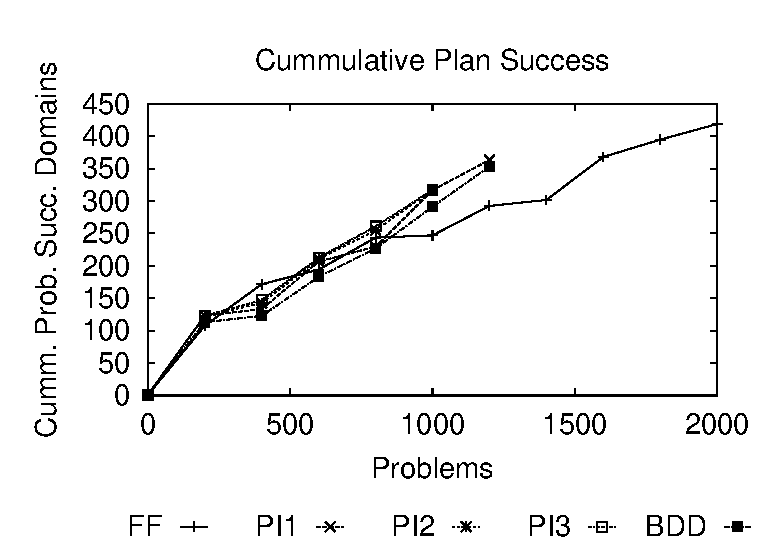
\includegraphics[width=.9\linewidth]{./alldom-deadline.eps}\\
% 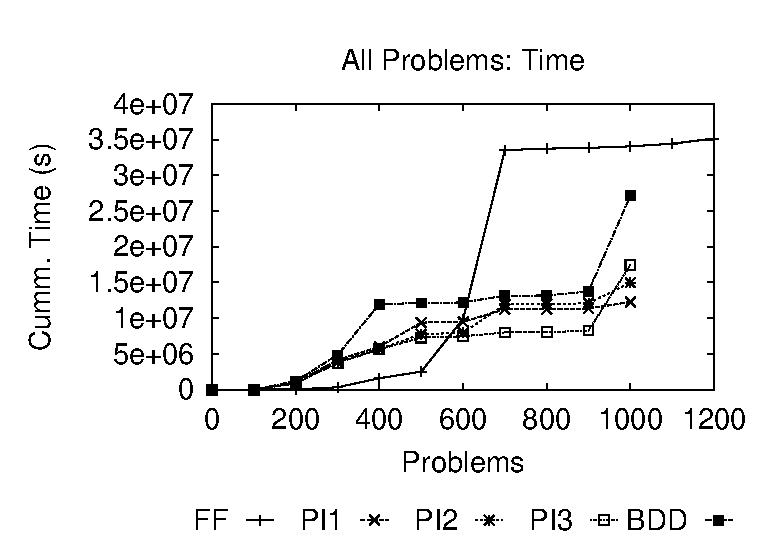
\includegraphics[width=.9\linewidth]{./alldom-deadline-time.eps}
% \caption{\label{fig:plan} Cumulative Plan Success and Planning Time}
% \end{figure}
 

\begin{table}\small\centering \begin{tabular}{|l|rrrrr|}      \hline &  FF  & 
PI1 & PI2  &  PI3  &  BDD  \\\hline
FF	&		0		&		155		&		161		&		161		&		123		\\
PI1	&	{\bf	629}	&		0		&	{\bf	79}	&	{\bf	78}	&	{\bf	208}	\\
PI2	&	{\bf	619}	&		77		&		0		&		46		&	{\bf	208}	\\
PI3	&	{\bf	594}	&		62		&	{\bf	51}	&		0		&	{\bf	199}	\\
BDD & {\bf 512} &  189  &  189  &  187  &  0  \\\hline
\end{tabular}																						
\caption{\label{tab:qualcomp} Num Instances with Better Quality.}
\end{table}

\begin{figure}\centering
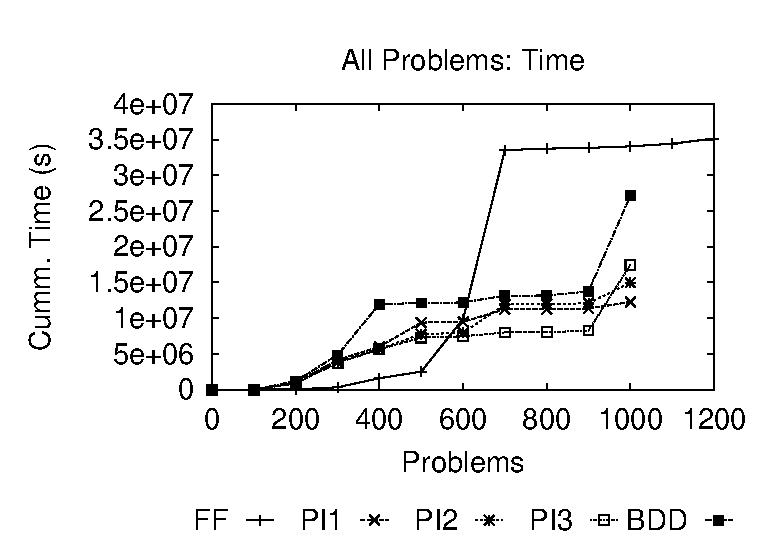
\includegraphics[width=\linewidth]{alldom-deadline-time.eps}
\caption{\label{fig:alltotaltime}Cumulative Time  in  All Domains.}
\end{figure} 
   
  
\begin{figure*}[t]    
\hspace*{-1cm}
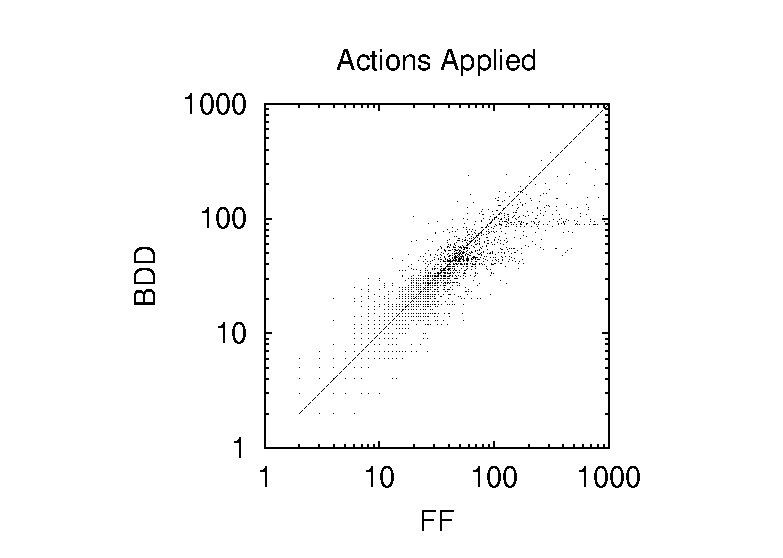
\includegraphics[width=.42\linewidth]{./hobonavSteps.eps}\hspace*{-1.5cm}
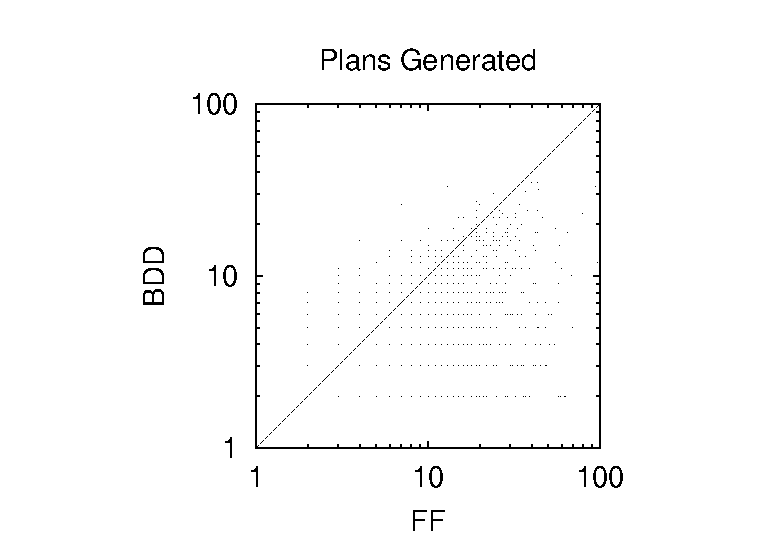
\includegraphics[width=.42\linewidth]{./hobonavPlans.eps}\hspace*{-1.5cm}
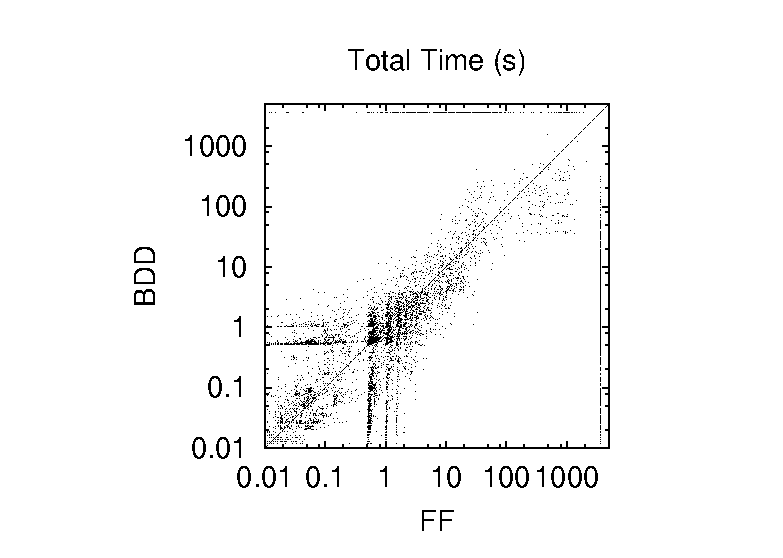
\includegraphics[width=.42\linewidth]{./hobonavTime.eps} 
%\hspace*{-2.25cm}       
%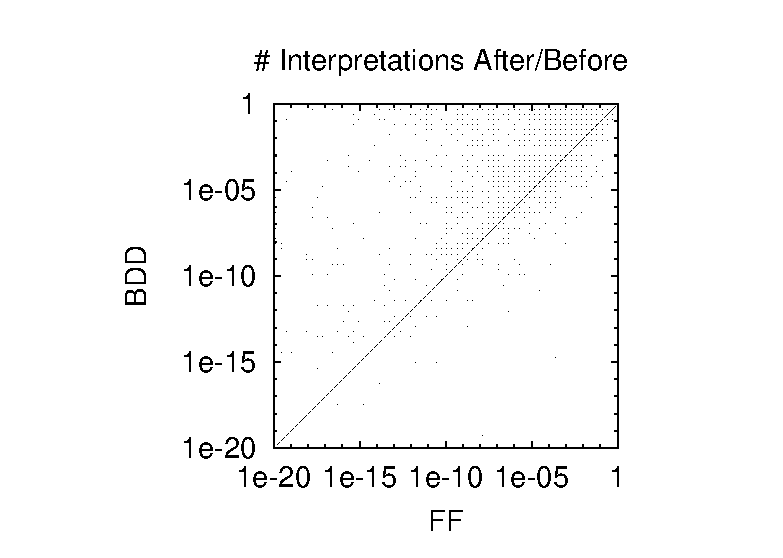
\includegraphics[width=.4\linewidth]{./hobonavLearning.eps}
\caption{\label{fig:exec} Comparison of Goalie with \FFRISKY-$FF$ and
\FFRISKY-$PI1$.}
\end{figure*}		   

 
% 
% \begin{table}\small
% \centering
% \begin{tabular}{|l|r|rrrr|r|}
% \hline
% Domain	&		{ FF}		&		{ PI1}		&		{ PI2}		&		{ PI3}		&		{
% BDD}		& { POND}	\\ 
% \hline \hline 
% PP 0.25	&		130		&		83		&		85		&	{\bf	86}	&		80		&	10	\\
% PP 0.5	&		130		&		87		&	{\bf	88}	&		87		&		80		&	0	\\
% PP 0.75	&		130		&		82		&	{\bf	83}	&		81		&		80		&	0	\\
% PP 1.0	&		13		&	{\bf	10}	&		9		&		9		&		8		&	0	\\	\hline
% PP	&		403		&		262		&	{\bf	265}	&		263		&		248		&	10	\\	\hline\hline
% BR1 0.25 	&		33		&	{\bf	19}	&	{\bf	19}	&	{\bf	19}	&	{\bf	19}	&	2	\\
% BR1 0.5 	&		33		&	{\bf	15}	&	{\bf	15}	&	{\bf	15}	&	{\bf	15}	&	2	\\
% BR1 0.75 	&		32		&	{\bf	18}	&		17		&		17		&	{\bf	18}	&	2	\\
% BR1 1.0 	&		4		&	{\bf	2}	&	{\bf	2}	&		1		&	{\bf	2}	&	1	\\
% BR2 0.25 	&		29		&		15		&	{\bf	16}	&	{\bf	16}	&	{\bf	16}	&	3	\\
% BR2 0.5 	&		31		&		16		&		12		&		12		&	{\bf	19}	&	3	\\
% BR2 0.75 	&		31		&		13		&		14		&		15		&	{\bf	16}	&	2	\\
% BR2 1.0 	&		4		&		1		&		1		&		0		&	{\bf	2}	&	1	\\
% BR3 0.25 	&		36		&		25		&		25		&		25		&	{\bf	26}	&	1	\\
% BR3 0.5 	&		37		&		22		&		22		&		22		&	{\bf	23}	&	2	\\
% BR3 0.75 	&		38		&	{\bf	25}	&	{\bf	25}	&		24		&	{\bf	25}	&	1	\\
% BR3 1.0 	&		4		&	{\bf	3}	&	{\bf	3}	&	{\bf	3}	&		2		&	1	\\	\hline
% BR 	&		312		&		174		&		171		&		169		&	{\bf	183}	&	21	\\	\hline\hline
% BW 0.25 	&		150		&		106		&		128		&	{\bf	129}	&		108		&	60	\\
% BW 0.5 	&		150		&		134		&	{\bf	137}	&		134		&		118		&	45	\\
% BW 0.75 	&		150		&	{\bf	140}	&		138		&		137		&		111		&	27	\\
% BW 1.0 	&		15		&	{\bf	14}	&	{\bf	14}	&	{\bf	14}	&		11		&	2	\\	\hline
% BW 	&		465		&		394		&	{\bf	417}	&		414		&		348		&	155	\\	\hline\hline
% PW 0.25 	&		160		&	{\bf	40}	&	{\bf	40}	&	{\bf	40}	&	{\bf	40}	&	19	\\
% PW 0.5 	&		160		&	{\bf	70}	&		60		&		50		&		60		&	13	\\
% PW 0.75 	&		170		&	{\bf	60}	&		50		&		40		&	{\bf	60}	&	12	\\
% PW 1.0 	&		19		&		5		&		6		&		6		&	{\bf	7}	&	2	\\	\hline
% PW 	&		509		&	{\bf	175}	&		156		&		136		&		167		&	46	\\	\hline\hline
% Total	&		1689		&		1005		&	{\bf	1009}	&		982		&		946		&	232	\\
% \hline
% \end{tabular}	\caption{\label{tab:solved} Instances Solved By Domain}
% \end{table}

\begin{table}				\small\centering																				
\begin{tabular}{|l|r|r@{ }r@{ }r@{ }r|r|}																								
\hline																								
Domain	&		FF		&		PI1		&		PI2		&		PI3		&		BDD		&	POND	\\ \hline	\hline
PP 0.25	&		130		&		83		&		85		&	{\bf	86}	&		80		&	10	\\	
PP 0.5	&		130		&		87		&	{\bf	88}	&		87		&		80		&	0	\\	
PP 0.75	&		130		&		82		&	{\bf	83}	&		81		&		80		&	0	\\	
PP 1.0	&		13		&	{\bf	10}	&		9		&		9		&		8		&	0	\\	\hline
PP	&		403		&		262		&	{\bf	265}	&		263		&		248		&	10	\\	\hline\hline
BR1 0.25 	&		40		&	{\bf	22}	&	{\bf	22}	&	{\bf	22}	&	{\bf	22}	&	2	\\	
BR1 0.5 	&		39		&	{\bf	20}	&	{\bf	20}	&	{\bf	20}	&	{\bf	20}	&	2	\\	
BR1 0.75 	&		36		&	{\bf	19}	&	{\bf	19}	&	{\bf	19}	&	{\bf	19}	&	2	\\	
BR1 1.0 	&		4		&	{\bf	2}	&	{\bf	2}	&	{\bf	2}	&	{\bf	2}	&	1	\\	
BR2 0.25 	&		38		&		20		&		20		&		20		&	{\bf	21}	&	3	\\	
BR2 0.5 	&		35		&	{\bf	25}	&	{\bf	25}	&	{\bf	25}	&		23		&	3	\\	
BR2 0.75 	&		35		&	{\bf	22}	&		21		&		21		&		21		&	2	\\	
BR2 1.0 	&		4		&	{\bf	2}	&	{\bf	2}	&	{\bf	2}	&	{\bf	2}	&	1	\\	
BR3 0.25 	&		45		&	{\bf	36}	&	{\bf	36}	&	{\bf	36}	&	{\bf	36}	&	1	\\	
BR3 0.5 	&		47		&	{\bf	33}	&	{\bf	33}	&	{\bf	33}	&		32		&	2	\\	
BR3 0.75 	&		46		&		39		&		39		&		39		&	{\bf	41}	&	1	\\	
BR3 1.0 	&		5		&	{\bf	4}	&	{\bf	4}	&	{\bf	4}	&		3		&	1	\\	\hline
BR 	&		374		&	{\bf	244}	&		243		&		243		&		242		&	21	\\	\hline\hline
BW 0.25 	&		150		&		106		&		128		&	{\bf	129}	&		108		&	60	\\	
BW 0.5 	&		150		&		134		&	{\bf	137}	&		134		&		118		&	45	\\	
BW 0.75 	&		150		&	{\bf	140}	&		138		&		137		&		111		&	27	\\	
BW 1.0 	&		15		&	{\bf	14}	&	{\bf	14}	&	{\bf	14}	&		11		&	2	\\	\hline
BW 	&		465		&		394		&	{\bf	417}	&		414		&		348		&	155	\\	\hline\hline
PW 0.25 	&		160		&	{\bf	40}	&	{\bf	40}	&	{\bf	40}	&	{\bf	40}	&	19	\\	
PW 0.5 	&		160		&	{\bf	70}	&		60		&		50		&		60		&	13	\\	
PW 0.75 	&		170		&	{\bf	60}	&		50		&		40		&	{\bf	60}	&	12	\\	
PW 1.0 	&		19		&		5		&		6		&		6		&	{\bf	7}	&	2	\\	\hline
PW 	&		509		&	{\bf	175}	&		156		&		136		&		167		&	46	\\	\hline\hline
Total	&		1751		&		1075		&	{\bf	1081}	&		1056		&		1005		&	232	\\	
\hline																								
\end{tabular}	\caption{\label{tab:solved} Instances Solved By Domain}																							
\end{table}																																												

% 
% \begin{table}																					
% \begin{tabular}{|l|r|rrrr|}																						
% \hline																						
% Domain	&		FF		&		PI1		&		PI2		&		PI3		&		BDD		\\ \hline	\hline
% PARC Printer &169&97&97&100&{\bf	140}	\\	\hline\hline
% Bridges1 0.25 	&		40		&	{\bf	40}	&		39		&		39		&	{\bf	40}	\\	
% Bridges1 0.5 	&		40		&		35		&		34		&		34		&	{\bf	40}	\\	
% Bridges1 0.75 	&		40		&		31		&		30		&		30		&	{\bf	32}	\\	
% Bridges1 1.0 	&		40		&	{\bf	30}	&		20		&		20		&	{\bf	30}	\\	
% Bridges2 0.25 	&		40		&		39		&		39		&		39		&	{\bf	40}	\\	
% Bridges2 0.5 	&		40		&		34		&		35		&		33		&	{\bf	40}	\\	
% Bridges2 0.75 	&		40		&	{\bf	31}	&		29		&		30		&		30		\\	
% Bridges2 1.0 	&		40		&	{\bf	30}	&		29		&		28		&	{\bf	30}	\\	
% Bridges3 0.25 	&		40		&	{\bf	40}	&	{\bf	40}	&	{\bf	40}	&	{\bf	40}	\\	
% Bridges3 0.5 	&		40		&	{\bf	40}	&	{\bf	40}	&	{\bf	40}	&	{\bf	40}	\\	
% Bridges3 0.75 	&		40		&		38		&		38		&		38		&	{\bf	40}	\\	
% Bridges3 1.0 	&		40		&	{\bf	37}	&	{\bf	37}	&		36		&		36		\\	\hline
% Bridges Total 	&		480		&		425		&		410		&		407		&	{\bf	438}	\\	\hline\hline
% Barter 0.25 	&		120		&	{\bf	120}	&	{\bf	120}	&	{\bf	120}	&	{\bf	120}	\\	
% Barter 0.5 	&		120		&	{\bf	120}	&	{\bf	120}	&	{\bf	120}	&		117		\\	
% Barter 0.75 	&		120		&	{\bf	120}	&		119		&	{\bf	120}	&		111		\\	
% Barter 1.0 	&		12		&	{\bf	12}	&	{\bf	12}	&	{\bf	12}	&		11		\\	\hline
% Barter Total 	&		372		&	{\bf	372}	&		371		&	{\bf	372}	&		359		\\	\hline\hline
% Pathways 0.25 	&		140		&		50		&		40		&		40		&	{\bf	60}	\\	
% Pathways 0.5 	&		140		&	{\bf	70}	&		60		&		50		&		60		\\	
% Pathways 0.75 	&		150		&	{\bf	60}	&		40		&		40		&	{\bf	60}	\\	
% Pathways 1.0 	&		170		&		50		&		60		&		60		&	{\bf	70}	\\	\hline
% Pathways Total	&		600		&		230		&		200		&		190		&	{\bf	250}	\\	\hline\hline
% Total	&		1621		&		1124		&		1078		&		1069		&	{\bf	1187}	\\	
% \hline														
% \end{tabular}	\caption{\label{tab:solved} Instances Solved By Domain}																					
% \end{table}																									
% 								



\und{On-line Planning and Execution Results} Figure \ref{fig:exec} depicts a
comparison between Goalie using \FFRISKY{}-$FF$ and \FFRISKY{}-$BDD$ to
synthesize plans, so that we can judge whether planning and execution strategies
such as that of CA will benefit from planners reason about incompleteness.  The
scatter plots in the figure show the respective number of actions applied to
achieve the goal, the number of plans generated, and the total planning and execution time.  

Q3 is answered mostly negatively. 
The plot of the total time taken shows that the planners are somewhat mixed or even for
times less than 10 seconds.  However, for times greater than 10 seconds, it
appears that using \FFRISKY-$FF$ in \goalie{} can take up to an order of
magnitude less time.  However, there are several difficult instances in
which \FFRISKY-$PI1$ does outperform \FFRISKY-$FF$.  By investigating the plots
of the number of actions taken and the number of plans generated, it is apparent
that \FFRISKY-$PI1$ takes fewer actions as the instances require near 100 steps,
and tends to re-plan less often.  We expect that more efficient implementations
of reasoning about prime implicants (e.g., tries) could lower the cost of
planning with \FFRISKY{}, making it able to capitalize on its better quality
plans.


% Another interesting observation is that the fourth plot in Figure \ref{fig:exec}
% indicates that upon goal achievement  \FFRISKY-$BDD$ typically eliminates fewer
% of the possible interpretations of incomplete domain than \FFRISKY-$FF$.  The
% explanation for this outcome is that by failing less, there is less opportunity
% to learn from failures, and by taking fewer actions overall, there are fewer
% actions that can be learned about.


%We discuss the results in each domain, and conclude this section with a discussion of the trends seen across the domains.  In several of the domains, we discuss alternative versions of the domain that include increasingly more incompleteness (measured by the number of incomplete features).  In all of the results plots, the legend refers to a configuration of the planner $X$, denoting \FFRISKY{}-$X$ (as described above).
%
%\und{Blind Navigation}  Figure \ref{fig:blindnav} shows that the \FFRISKY{}-$FF$ configuration finds plans of comparable quality to the configurations that reason about incompleteness only in the smallest instances (instances 1-10, which are 2x2 grids).  Each additional ten instances increase the grid size to 4x4, 8x8, and 16x16.  The \FFRISKY{}-$FF$, and \FFRISKY{}-$1$, $-2$, or $-3$ configurations cannot solve instances bigger than 8x8, due to the importance of reasoning about incompleteness in this domain.  It appears that approximating the failed interpretations of the domain does not harm the quality of plans, but it does limit the scalability.
%
%\begin{figure}
%%\includegraphics[width=1\linewidth]{plot/blindnav.eps}
%\includegraphics[width=.5\linewidth]{jplot/blindnav-deadline.eps}
%\includegraphics[width=.5\linewidth]{jplot/blindnav-deadline-time.eps}
%\caption{\label{fig:blindnav} Cumulative Quality and Time Comparison in Blind Navigation Domain.}
%\end{figure}
%
%\und{Parc Printer}  Figure \ref{fig:BR} shows reasoning about incompleteness in the Parc Printer domain is important to finding high quality plans, but not necessarily important to finding plans.  The \FFRISKY{}-$FF$ configuration scales well, but finds the worst quality plans.  The \FFRISKY{}-$1$, $-2$, and $-3$  configurations find the highest quality plans (which are identical quality), but do not scale as well as \FFRISKY{}-$All$.  The difference between model counting and prime implicant counting in this domain may be attributed to the potentially efficient OBDD representation of the failed domain interpretations, but fortuitous prime implicant representation that helps identify other, better plans.
%
%
%\begin{figure}
%%\includegraphics[width=.5\linewidth]{jplot/parcprinter.eps}
%\includegraphics[width=.5\linewidth]{jplot/parcprinter-deadline.eps}
%\includegraphics[width=.5\linewidth]{jplot/parcprinter-deadline-time.eps}
%\caption{\label{fig:parcprinter}Cumulative Quality and Time Comparison in  Parc Printer Domain.}
%\end{figure}
%
%
%\und{Bridges} Figure \ref{fig:bridges} shows results for all three versions of the domain combined, and Figures \ref{fig:bridges1}, \ref{fig:bridges2}, \ref{fig:bridges3} show the results for the respective versions of the domain.  Common to all versions of the domain, \FFRISKY{}-$FF$ finds the poorest quality plans, but surprisingly is not overly superior in terms of planning time and problems solved.  
%In all versions of the domain, the \FFRISKY{}-$1$ configuration solves the most problems, and in the third version of the domain it has the best overall planning time.  However, considering more faulty interpretations, either by using \FFRISKY{}-$1$, $-2$, or $All$, does improve plan quality at the expense of scalability and planning time.  Interestingly, the trends remain the same across the versions of the domain, with \FFRISKY{}-$FF$ performing progressively worse as we include different types of incomplete domain features.
%
%\begin{figure}
%%\includegraphics[width=1\linewidth]{plot/bridges.eps}
%\includegraphics[width=.5\linewidth]{jplot/bridges-deadline.eps}
%\includegraphics[width=.5\linewidth]{jplot/bridges-deadline-time.eps}
%\caption{\label{fig:bridges} Cumulative Quality and Time Comparison in three versions of the Bridges Domain.}
%\end{figure}
%
%\begin{figure}
%%\includegraphics[width=1\linewidth]{plot/bridges1.eps}
%\includegraphics[width=.5\linewidth]{jplot/bridges1-deadline.eps}
%\includegraphics[width=.5\linewidth]{jplot/bridges1-deadline-time.eps}
%\caption{\label{fig:bridges1} Cumulative Quality and Time Comparison in version one of the Bridges Domain.}
%\end{figure}
%
%\begin{figure}
%%\includegraphics[width=1\linewidth]{plot/bridges2.eps}
%\includegraphics[width=.5\linewidth]{jplot/bridges2-deadline.eps}
%\includegraphics[width=.5\linewidth]{jplot/bridges2-deadline-time.eps}
%\caption{\label{fig:bridges2} Cumulative Quality and Time Comparison in version two of the Bridges Domain.}
%\end{figure}
%
%\begin{figure}
%%\includegraphics[width=.5\linewidth]{plot/bridges3.eps}
%\includegraphics[width=.5\linewidth]{jplot/bridges3-deadline.eps}
%\includegraphics[width=.5\linewidth]{jplot/bridges3-deadline-time.eps}
%\caption{\label{fig:bridges3} Cumulative Quality and Time Comparison in version three of the Bridges Domain.}
%\end{figure}
%
%
%\und{Barter World}  Figure \ref{fig:barter} shows the combined results for four versions of the Barter World domain, which are shown individually in Figures \ref{fig:barter25}, \ref{fig:barter5}, \ref{fig:barter75}, and \ref{fig:barter1}, which respectively setting the probability of the domain generator introducing incomplete features to 0.25, 0.5, 0.75, and 1.0.  
%
%The trend identified by \ref{fig:barter} is that failing to reason about incompleteness permits greater scalability, but poor quality plans, and as the reasoning about incompleteness strengthens, so does the plan quality (but at the expense of scalability).  As the number of incomplete features grows across Figures \ref{fig:barter25} to \ref{fig:barter1}, we see the same trend exacerbated: weaker reasoning about incompleteness scales better, and stronger reasoning finds better quality plans.
%
%\begin{figure}
%%
%%\includegraphics[width=.5\linewidth]{plot/hobonav.eps}
%\includegraphics[width=.5\linewidth]{jplot/hobonav-deadline.eps}
%\includegraphics[width=.5\linewidth]{jplot/hobonav-deadline-time.eps}
%%
%\caption{\label{fig:barter} Cumulative Quality and Time Comparison in all instances of Barter World Domain.}
%\end{figure}
%
%\begin{figure}
%%\includegraphics[width=.5\linewidth]{jplot/hobonav_0.25.eps}
%\includegraphics[width=.5\linewidth]{jplot/hobonav_0.25-deadline.eps}
%\includegraphics[width=.5\linewidth]{jplot/hobonav_0.25-deadline-time.eps}
%\caption{\label{fig:barter25} Cumulative Quality and Time Comparison in 0.25 density Barter World Domain.}
%\end{figure}
%
%\begin{figure}
%%\includegraphics[width=.5\linewidth]{jplot/hobonav_0.5.eps}
%\includegraphics[width=.5\linewidth]{jplot/hobonav_0.5-deadline.eps}
%\includegraphics[width=.5\linewidth]{jplot/hobonav_0.5-deadline-time.eps}
%\caption{\label{fig:barter5} Cumulative Quality and Time Comparison in 0.5 density Barter World Domain.}
%\end{figure}
%
%\begin{figure}
%%\includegraphics[width=.5\linewidth]{jplot/hobonav_0.75.eps}
%\includegraphics[width=.5\linewidth]{jplot/hobonav_0.75-deadline.eps}
%\includegraphics[width=.5\linewidth]{jplot/hobonav_0.75-deadline-time.eps}
%\caption{\label{fig:barter75} Cumulative Quality and Time Comparison in 0.75 density Barter World Domain.}
%\end{figure}
%
%\begin{figure}
%%\includegraphics[width=.5\linewidth]{jplot/hobonav_1.0.eps}
%\includegraphics[width=.5\linewidth]{jplot/hobonav_1.0-deadline.eps}
%\includegraphics[width=.5\linewidth]{jplot/hobonav_1.0-deadline-time.eps}
%\caption{\label{fig:barter1}Cumulative Quality and Time Comparison in 1.0 density Barter World Domain.}
%\end{figure}
%
%
%\und{Pathways}  Figure \ref{fig:pathways} shows the combined results for four versions of the Pathways domain that set the probability of generating incomplete domain features to 0.25, 0.5, 0.75, and 1.0.  The results for each of the settings are shown individually in Figures \ref{fig:pathways_0.25}, \ref{fig:pathways_0.5}, \ref{fig:pathways_0.75}, and \ref{fig:pathways_1.0}.
%
%The combined results demonstrate that the techniques for reasoning about incompleteness find similar quality plans, but the weaker the technique, the lower its planning time.  As the probability of including incomplete features increases, the stronger reasoning about incompleteness does not scale as well, but the quality of the plans found by the techniques is similar.
%
%\begin{figure}
%%\includegraphics[width=.5\linewidth]{jplot/pathways.eps}
%\includegraphics[width=.5\linewidth]{jplot/pathways-deadline.eps}
%\includegraphics[width=.5\linewidth]{jplot/pathways-deadline-time.eps}
%\caption{\label{fig:pathways}Cumulative Quality and Time Comparison in Pathways Domain.}
%\end{figure}
%
%\begin{figure}
%%\includegraphics[width=.5\linewidth]{jplot/pathways.eps}
%\includegraphics[width=.5\linewidth]{jplot/pathways_0.25-deadline.eps}
%\includegraphics[width=.5\linewidth]{jplot/pathways_0.25-deadline-time.eps}
%\caption{\label{fig:pathways_0.25}Cumulative Quality and Time Comparison in 0.25 density Pathways Domain.}
%\end{figure}
%
%\begin{figure}
%%\includegraphics[width=.5\linewidth]{jplot/pathways.eps}
%\includegraphics[width=.5\linewidth]{jplot/pathways_0.5-deadline.eps}
%\includegraphics[width=.5\linewidth]{jplot/pathways_0.5-deadline-time.eps}
%\caption{\label{fig:pathways_0.5}Cumulative Quality and Time Comparison in 0.5 density Pathways Domain.}
%\end{figure}
%
%\begin{figure}
%%\includegraphics[width=.5\linewidth]{jplot/pathways.eps}
%\includegraphics[width=.5\linewidth]{jplot/pathways_0.75-deadline.eps}
%\includegraphics[width=.5\linewidth]{jplot/pathways_0.75-deadline-time.eps}
%\caption{\label{fig:pathways_0.75}Cumulative Quality and Time Comparison in 0.75 density Pathways Domain.}
%\end{figure}
%
%\begin{figure}
%%\includegraphics[width=.5\linewidth]{jplot/pathways.eps}
%\includegraphics[width=.5\linewidth]{jplot/pathways_1.0-deadline.eps}
%\includegraphics[width=.5\linewidth]{jplot/pathways_1.0-deadline-time.eps}
%\caption{\label{fig:pathways_1.0}Cumulative Quality and Time Comparison in 1.0 density Pathways Domain.}
%\end{figure}
%
%\und{Discussion} As the strength of the reasoning about incompleteness increases from ignoring incompleteness to tracking increasingly higher cardinality prime implicants, to tracking all interpretations of an incomplete domain, we tend to see increasing plan quality, in terms of the number of domain interpretations that will successfully execute the plan and achieve the goal.  We also see scalability decrease as a result.  Reasoning about prime implicants tends to be a useful middle-ground whereby plans have good quality, and planner scalability is best.  
%
%
%%By Domain, plot 
%% i) proportion solved by instance by num features
%% ii) runtime by instance by num features
%% iii) plan length by instance by num features
%% Table with all domains, show num instances solved 
%
%
%
%%\und{Results} The first set of results depicted in Figure \ref{pathwaysResults} illustrates the impact of increasing the level of incompleteness of problems in Pathways.  The figure shows three instances (p02, p05, and p09) where the top row of plots is the average, minimum, and maximum number of critical faults (including the maximum possible, independent of the planner result) and the bottom row is the total planner time in seconds.  The horizontal axis denotes the probability of injecting incompleteness, described above. The planners compared are POND, the control planner using only $h^{FF}$ (denoted FF), \FFRISKY{} using the $h^{\sim}$ (fault) heuristic and $h^{\sim FF}$ (length) to break ties (denoted FFR-RL), and \FFRISKY{} using the $h^{\sim FF}$ heuristic and $h^{\sim}$ to break ties (denoted FFR-LR).  Both FFR-RL and FFR-LR use the multiple supporter fault propagation approach in the planning graph.  The results are offset in the graph for better clarity, but results for the same density are centered on the axis tics.  
%%
%%	
%%
%%There are several points to note about the Pathways comparisons: POND does not scale well in either the instance size or the level of incompleteness, the control planner performs worst in terms of critical faults but best in terms of time, FFR-RL finds the best quality plans but takes the longest, and FFR-LR generally improves runtime and scalability over FFR-RL.  POND has limited applicability because its precision (representing state distributions) is exceeded as the total number of faults increases, but even if the issue is resolved it does not appear to be competitive.  As expected, ignoring faults in the control planner leads to good scalability but poor plans.  The difference between FFR-RL and FFR-LR is that measuring fault as the primary heuristic estimator leads to considerably more search (as fault does not correlate with the number of nodes expanded along a path to a solution, whereas estimates of plan length do).  The increased search performed by FFR-RL limits its scalability, but using FFR-LR is a reasonable alternative that scales better.  
%%
%%\begin{table*}
%%																	
%%
%%\scalebox{.9}{
%%
%%\begin{tabular}{|l||r||c|c|c|c|c|c|}							\hline																																			
%%Prob	&	Risks	&	FF					&		FFR-LR-SS						&		FFR-LR-MS				&		FFR-RL-SS						&		FFR-RL-MS				&	POND			\\ \hline	\hline
%%BN-2	&	22	&	2.00	/	{\bf 	0.08	} 	&		2.00		/		0.17		&		2.00		/	0.18	&		0.67		/		0.22		&	{\bf 	0.56	} 	/	0.29	&	1.46	/	0.54	\\ \hline	
%%BN-4	&	124	&	6.00	/	{\bf 	0.44	} 	&		6.00		/		0.94		&		6.00		/	0.96	&		1.50		/		1.19		&	{\bf 	0.43	} 	/	8.53	&	-	/	-	\\ \hline	
%%BN-6	&	310	&	10.00	/	{\bf 	1.10	} 	&		10.00		/		2.89		&		10.00		/	3.34	&		5.43		/		4.55		&	{\bf 	1.50	} 	/	68.31	&	-	/	-	\\ \hline	\hline
%%B1-2	&	4	&	2.80	/	{\bf 	0.07	} 	&	{\bf 	2.00	} 	/		0.13		&	{\bf 	2.00	} 	/	0.14	&	{\bf 	2.00	} 	/		0.15		&	{\bf 	2.00	} 	/	0.16	&	3.30	/	0.20	\\ \hline	
%%B1-4	&	24	&	7.30	/	{\bf 	0.82	} 	&		4.70		/		0.84		&		4.70		/	0.88	&	{\bf 	3.00	} 	/		1.12		&	{\bf 	3.00	} 	/	1.13	&	15.00	/	224.00	\\ \hline	
%%B1-8	&	112	&	-	/		-		&		13.20		/		87.41		&		13.20		/	102.70	&	{\bf 	6.00	} 	/	{\bf 	6.23	} 	&	{\bf 	6.00	} 	/	7.36	&	-	/	-	\\ \hline	
%%B1-16	&	480	&	-	/		-		&		-		/		-		&		-		/	-	&		-		/		-		&		-		/	-	&	-	/	-	\\ \hline	\hline
%%B2-2	&	16	&	2.80	/	{\bf 	0.07	} 	&	{\bf 	2.00	} 	/		0.13		&	{\bf 	2.00	} 	/	0.14	&	{\bf 	2.00	} 	/		0.18		&	{\bf 	2.00	} 	/	0.19	&	3.00	/	0.49	\\ \hline	
%%B2-4	&	63	&	8.50	/	{\bf 	0.87	} 	&		5.90		/		1.05		&		5.90		/	1.09	&	{\bf 	1.00	} 	/		1.00		&	{\bf 	1.00	} 	/	1.01	&	-	/	-	\\ \hline	
%%B2-8	&	307	&	-	/		-		&	{\bf 	12.78	} 	/	{\bf 	195.45	} 	&	{\bf 	12.78	} 	/	237.59	&		-		/		-		&		-		/	-	&	-	/	-	\\ \hline	
%%B2-16	&	1278	&	-	/		-		&		-		/		-		&		-		/	-	&		-		/		-		&		-		/	-	&	-	/	-	\\ \hline	\hline
%%B3-2	&	17	&	1.60	/	{\bf 	0.05	} 	&		1.40		/		0.10		&		1.40		/	0.11	&	{\bf 	1.33	} 	/		0.14		&		1.44		/	0.15	&	3.78	/	0.46	\\ \hline	
%%B3-4	&	76	&	4.20	/	{\bf 	0.29	} 	&		3.20		/		0.51		&		3.20		/	0.55	&	{\bf 	2.20	} 	/		0.74		&	{\bf 	2.20	} 	/	0.79	&	-	/	-	\\ \hline	
%%B3-8	&	313	&	11.38	/		12.35		&		9.20		/		54.76		&		9.20		/	67.76	&	{\bf 	0.00	} 	/	{\bf 	3.25	} 	&	{\bf 	0.00	} 	/	3.63	&	-	/	-	\\ \hline	
%%B3-16	&	1264	&	16.00	/	{\bf 	128.07	} 	&	{\bf 	11.00	} 	/		476.71		&	{\bf 	11.00	} 	/	546.75	&		-		/		-		&		-		/	-	&	-	/	-	\\ \hline
%%\end{tabular}																																																																																																																
%%
%%%
%%%\begin{tabular}{|l||r||c|c|c|c|c|c|}									\hline																																											
%%%Prob	&	Risks	&		POND						&		FF						&		FFR-RL-SS						&		FFR-RL-MS						&		FFR-LR-SS						&		FFR-LR-MS						\\ \hline	\hline
%%%BN-2	&	22	&		1.46		/		0.54		&		2.00		/	{\bf 	0.08	} 	&		0.67		/		0.22		&	{\bf 	0.56	} 	/		0.29		&		2.00		/		0.17		&		2.00		/		0.18		\\ \hline	
%%%BN-4	&	124	&		-		/		-		&		6.00		/	{\bf 	0.44	} 	&		1.50		/		1.19		&	{\bf 	0.43	} 	/		8.53		&		6.00		/		0.94		&		6.00		/		0.96		\\ \hline	
%%%BN-6	&	310	&		-		/		-		&		10.00		/	{\bf 	1.10	} 	&		5.43		/		4.55		&	{\bf 	1.50	} 	/		68.31		&		10.00		/		2.89		&		10.00		/		3.34		\\ \hline	\hline
%%%B1-2	&	4	&		3.30		/		0.20		&		2.80		/	{\bf 	0.07	} 	&	{\bf 	2.00	} 	/		0.15		&	{\bf 	2.00	} 	/		0.16		&	{\bf 	2.00	} 	/		0.13		&	{\bf 	2.00	} 	/		0.14		\\ \hline	
%%%B1-4	&	24	&		15.00		/		224.00		&		7.30		/	{\bf 	0.82	} 	&	{\bf 	3.00	} 	/		1.12		&	{\bf 	3.00	} 	/		1.13		&		4.70		/		0.84		&		4.70		/		0.88		\\ \hline	
%%%B1-8	&	112	&		-		/		-		&		-		/		-		&	{\bf 	6.00	} 	/	{\bf 	6.23	} 	&	{\bf 	6.00	} 	/		7.36		&		13.20		/		87.41		&		13.20		/		102.70		\\ \hline	
%%%B1-16	&	480	&		-		/		-		&		-		/		-		&		-		/		-		&		-		/		-		&		-		/		-		&		-		/		-		\\ \hline	\hline
%%%B2-2	&	16	&		3.00		/		0.49		&		2.80		/	{\bf 	0.07	} 	&	{\bf 	2.00	} 	/		0.18		&	{\bf 	2.00	} 	/		0.19		&	{\bf 	2.00	} 	/		0.13		&	{\bf 	2.00	} 	/		0.14		\\ \hline	
%%%B2-4	&	63	&		-		/		-		&		8.50		/	{\bf 	0.87	} 	&	{\bf 	1.00	} 	/		1.00		&	{\bf 	1.00	} 	/		1.01		&		5.90		/		1.05		&		5.90		/		1.09		\\ \hline	
%%%B2-8	&	307	&		-		/		-		&		-		/		-		&		-		/		-		&		-		/		-		&	{\bf 	12.78	} 	/	{\bf 	195.45	} 	&	{\bf 	12.78	} 	/		237.59		\\ \hline	
%%%B2-16	&	1278	&		-		/		-		&		-		/		-		&		-		/		-		&		-		/		-		&		-		/		-		&		-		/		-		\\ \hline	\hline
%%%B3-2	&	17	&		3.78		/		0.46		&		1.60		/	{\bf 	0.05	} 	&	{\bf 	1.33	} 	/		0.14		&		1.44		/		0.15		&		1.40		/		0.10		&		1.40		/		0.11		\\ \hline	
%%%B3-4	&	76	&		-		/		-		&		4.20		/	{\bf 	0.29	} 	&	{\bf 	2.20	} 	/		0.74		&	{\bf 	2.20	} 	/		0.79		&		3.20		/		0.51		&		3.20		/		0.55		\\ \hline	
%%%B3-8	&	313	&		-		/		-		&		11.38		/		12.35		&	{\bf 	0.00	} 	/	{\bf 	3.25	} 	&	{\bf 	0.00	} 	/		3.63		&		9.20		/		54.76		&		9.20		/		67.76		\\ \hline	
%%%B3-16	&	1264	&		-		/		-		&		16.00		/	{\bf 	128.07	} 	&		-		/		-		&		-		/		-		&	{\bf 	11.00	} 	/		476.71		&	{\bf 	11.00	} 	/		546.75		\\ \hline
%%%\end{tabular}																																																																																																																						
%%}																																																																																																																		
%%\caption{\label{tab:results} \small\it Average ``Critical Risks/Time (s)'' results for Blind Navigator (BN-X) and Bridges (BY-X) versions Y= \{1, 2, 3\} and grid sizes X = \{2, 4, 6, 8, 16\}.  Planners, ordered roughly by speed and quality from left to right, include the control planner ``FF'', and \FFRISKY{} ``FFR'' with either single ``SS'' or multiple ``MS'' supporters for propositions in the heuristic and either using relaxed plan length as the primary heuristic and fault as the tie breaking heuristic ``LR'' or vice versa ``RL'', and POND.  Results exceeding the time limit are denoted by ``-/-''. The best number of faults and time for each instance are in bold.
%%}
%%\end{table*}	
%%
%%Another interesting trend in Pathways is that as the size of the instances increases, difficulty shifts from instances with high incompleteness to instances with low incompleteness.  An explanation for this observation is that in small problems (plan lengths around 10 in p02, and around 25 in p05) there are many more possible plans as the incompleteness increases, leading to heuristic plateaus.  However, in large problems (plan lengths around 50-70 in p09) increased incompleteness decreases the plan length, making the problems easier.  
%%
%%Table \ref{tab:results} lists results for the Blind Navigator and Bridges domains.  In these domains we additionally compare the effect of using multiple supporters for propositions in the relaxed planning graphs to selecting single supporters; the impact is most noticeable in the Blind Navigator domain.  In all instances of Blind Navigator, using multiple supporters reduces the number of critical faults, which is expected because the domain was engineered so that plans using more observation actions to localize the navigator will have fewer faults.  The Bridges domains support many of the same conclusions drawn from the Pathways domain: i) using relaxed plan length as the primary heuristic (LR) leads to better scalability, but increases fault, ii) the control planner is fast, but finds poor quality plans, and iii)  \FFRISKY{} outscales POND.  One unique aspect of Bridges is the manner in which each version adds a different type of incompleteness, and it is interesting to see how \FFRISKY{} responds.  For example, from Bridges1 to Bridges2 we add possible delete effects and performance suffers, but from Bridges2 to Bridges3 we add possible add effects and performance improves.  This result is also expected because the \FFRISKY{} heuristics ignore delete effects.
%%
%%\und{Summary}  Our experiments have demonstrated several useful lessons about planning in incomplete domains: i) reasoning about incompleteness leads to better quality (more-correct) plans, ii) using a heuristic that primarily measures the number of critical faults leads to better quality plans than a relaxed plan length based heuristic, but at the expense of better scalability, and iii) translating incomplete domains to CPP is not currently a viable approach.
%%%
%%%The results depicted in Table \ref{tab:results} compare \FFRISKY{} to the control planner on several problems (listed in each row).  The data presented for each planner are the measures mentioned above.  Instances in the DriverLog domain are prefixed by ``DL'' and instances in the Rovers domain are prefixed by ``R''.
%%
%%%
%%%\und{Rovers} The Rovers domain involves relatively fewer faults than the DriverLog domain, but we continue to see improvement in the number of critical faults with \FFRISKY{}.  In all cases, \FFRISKY{} finds plans with fewer faults.  The heuristic used by  \FFRISKY{} appears to be fairly weak because of the high number of additional expanded nodes, and the heuristic considerably raises the per node cost.  Yet, there are cases, like R4, where \FFRISKY{} finds a plan in fewer nodes.  It does appear that reducing fault increases plan cost, except in R3, where \FFRISKY{} dominates in all but search time.  Generally, \FFRISKY{} does not require many additional actions to improve fault.
%%
%%%\und{DriverLog}  The DriverLog domain exhibits trends that are similar to Rovers.  \FFRISKY{} requires more search nodes, but always finds better fault plans in sometimes fewer plan steps.  It appears that \FFRISKY{} has a weaker heuristic in this domain because it requires a higher proportion of search nodes over the control planner than in Rovers and fails to solve DL5.  The additional nodes is also likely to the plans admitting more faults.
%%
%%%
%%\und{Summary} While our sample size is relatively small, \FFRISKY{} does appear to reduce fault over the control planner and can scale reasonably well (without other search enhancements, such as those used in FF and other planners).  Interestingly, there are cases where \FFRISKY{} finds plans with fewer faults and a lower plan length than the control planner, but these seem to be rare.  We anticipate better scalability by using relaxed plans extracted from the fault propagated planning graph, but are encouraged by these preliminary results.
%%
%%
%%

\section{Related Work}

Planning in incomplete domains is noticeably similar to planning with incomplete
information, where action descriptions instead of states are incomplete. 
Incomplete domains can be translated to conformant probabilistic planning
domains, and planners such as POND \citep{aij-mclug} and PFF \citep{pff} are
applicable.  However, while the translation is theoretically feasible, practical
issues regarding numeric precision prohibit effective use of existing planners. 
While we do not report results, we translated the instances described here and
ran both POND and PFF; both planners compared equally with \FFRISKY{} on the
problems where numeric precision was not exceeded.

Our investigation is an instantiation of model-lite planning \citep{modellite}.  Constraint-based hierarchical task networks are an alternative, pointed out by \citet{modellite},  which avoid specifying all preconditions and effects through methods and constraints that correspond to underlying, implicit causal links.

As previously stated, this work is a natural extension of the \citet{Garland02} model for evaluating plans in incomplete domains.  Our methods for computing plan failure explanations are slightly different in that we compute them in the forward direction and allow for multiple, interacting faults instead of the single faults.  In addition to calculating the failure explanations of partial plans, we have also presented a relaxed planning heuristic informed by failure explanations.

Prior work of \citet{DBLP:conf/aips/ChangA06} addresses planning with incomplete models, but does not attempt to synthesize robust plans, which is similar to our \FFRISKY{}-$FF$ planner.  We have shown that incorporating knowledge about domain incompleteness into the planner can lead to a more effective agent.  We also differ in that we do not assume direct feedback from the environment about action failures and we can learn action preconditions.

\section{Conclusion}

We have presented the first work to address planning in incomplete domains as
heuristic search to find robust plans.  Our planner, \FFRISKY{}, i) performs
forward search while maintaining plan failure explanations, and ii) estimates
the future failures by propagating failure explanations on planning graphs.  We
have shown that, compared to a planner that essentially ignores aspects of the
incomplete domain, \FFRISKY{} is able to scale reasonably well but find much
better quality plans.  We have also shown that representing plan failure
explanations with prime implicants leads to better scalability than counting
OBDDs models.  Our agent \goalie{} is  effective when using \FFRISKY{}, can learn  incomplete
actions, and can diagnose future and past failures.

%Future work on this topic will focus on additional heuristics for estimating fault that incorporate possible clobberer faults and other negative interactions.  One direction for extending the heuristics will use interaction propagation to measure the cost added by possible or real mutexes \citep{interaction}.  We also intend to compare against the approach mentioned above that translates the incomplete action descriptions into incomplete states and uses a conformant planner.  Directions for extending our model of incompleteness include adding probabilistic measures of various action features existing in the true domain and how incompleteness can be integrated with uncertain/stochastic action effects.

\und{Acknowledgements} This work was supported by DARPA contract HR001-07-C-0060.
\footnotesize
\def\baselinestretch{0.7}
\bibliography{jared}
\bibliographystyle{abbrvnat}

%
%\subsection{Conformant Probabilistic Planning Domains}
%
%We will describe a formulation of planning in incomplete domains as conformant probabilistic planning that introduces state propositions corresponding to the fault literals.  Conformant planning deals with the problem of having a set of states (a belief state) consistent with an agent's knowledge and attempting to find a plan that will achieve the goals simultaneously from as many of the possible states.
%
%\begin{definition}
%A conformant probabilistic planning domain $\overline{D}$  defines the tuple ($\overline{P}$, $\overline{A}$, $\overline{b_I}$, $\overline{G}$, $\overline{\tau}$), where 
%
%\begin{packed_itemize}
%\item $\overline{P}$ is a set of propositions
%\item  $\overline{A}$ is a set of actions, where each $\overline{a} \in \overline{A}$ defines a set of conditional effects $\text{eff}(\overline{a}) = \{\text{eff}_0(\overline{a}), ..., \text{eff}_{m-1}(\overline{a})\}$.  Each conditional effect $\text{eff}_i(\overline{a})$ consists of 
%\begin{itemize}
%\item $\text{pre}_i(\overline{a}) \subseteq P$, a set of secondary preconditions
%\item $\text{add}_i(\overline{a}) \subseteq P$, a set of add effects
%\item $\text{del}_i(\overline{a}) \subseteq P$, a set of delete effects
%\end{itemize}
%We require that no two conditional effects conflict (i.e., there are no cases where two conditional effects are applicable in a state $s$ and they disagree on the effect on a proposition, $\text{pre}_i(\overline{a}) \subseteq s, \text{pre}_j(\overline{a}) \subseteq s$ and $\text{add}_i(\overline{a}) \cap \text{del}_j(\overline{a}) \not= \{\}$).
%\item $\overline{b_I}$ is the initial belief state, such that $\overline{b_I}(s) = Pr(s)$, for all $s \subseteq P$.
%\item $\overline{G}\subseteq P$ is the goal 
%\item $0 < \overline{\tau} \leq 1$ is a lower bound on the probability of goal satisfaction
%\end{packed_itemize}
%\end{definition}
%
%For example, the CPP translation (defined later) of the incomplete domain example defines:
%
%\begin{packed_itemize}
%\item $\overline{P} = \{p, np,  q, nq, r, nr, g, ng, valid, nvalid, f_0, nf_0, f_1, nf_1, f_2, nf_2, f_3, nf_3, f_4, nf_4\} $
%
%\item $\overline{A} = \{\overline{a}, \overline{b}, \overline{c}\}$
%
%$\begin{array}{lll}
%\text{pre}_0(\overline{a}) = \{p, q, valid, nf_0, nf_1, nf_2\} & \text{add}_0(\overline{a}) = \{r\} &   \text{del}_0(\overline{a}) = \{nr\}\\
%\text{pre}_1(\overline{a}) = \{p, q, valid, nf_0, nf_1, f_2\} & \text{add}_1(\overline{a}) = \{\} &   \text{del}_1(\overline{a}) = \{\}\\
%\text{pre}_2(\overline{a}) = \{p, q, valid, nf_0, f_1, nf_2\} & \text{add}_2(\overline{a}) = \{np, r\} &   \text{del}_2(\overline{a}) = \{p, nr\}\\
%\text{pre}_3(\overline{a}) = \{p, q, valid, nf_0, f_1, f_2\} & \text{add}_3(\overline{a}) = \{np\} &   \text{del}_3(\overline{a}) = \{p\}\\
%\text{pre}_4(\overline{a}) = \{p, q, r, valid, f_0, nf_1, nf_2\} & \text{add}_4(\overline{a}) = \{r\} &   \text{del}_4(\overline{a}) = \{nr\}\\
%\text{pre}_5(\overline{a}) = \{p, q, r, valid, f_0, nf_1, f_2\} & \text{add}_5(\overline{a}) = \{\} &   \text{del}_5(\overline{a}) = \{\}\\
%\text{pre}_6(\overline{a}) = \{p, q, r, valid, f_0, f_1, nf_2\} & \text{add}_6(\overline{a}) = \{np, r\} &   \text{del}_6(\overline{a}) = \{p, nr\}\\
%\text{pre}_7(\overline{a}) = \{p, q, r, valid, f_0, f_1, f_2\} & \text{add}_7(\overline{a}) = \{np\} &   \text{del}_7(\overline{a}) = \{p\}\\
%\text{pre}_8(\overline{a}) = \{nr, f_0\} & \text{add}_8(\overline{a}) = \{nvalid\} &   \text{del}_8(\overline{a}) = \{valid\}\\
%\text{pre}_9(\overline{a}) = \{np\} & \text{add}_9(\overline{a}) = \{nvalid\} &   \text{del}_9(\overline{a}) = \{valid\}\\
%\text{pre}_{10}(\overline{a}) = \{nq\} & \text{add}_{10}(\overline{a}) = \{nvalid\} &   \text{del}_{10}(\overline{a}) = \{valid\}\\
%\\
%\text{pre}_0(\overline{b}) = \{p, nf_3, valid\} & \text{add}_0(\overline{b}) = \{r\} &   \text{del}_0(\overline{b}) = \{nr\}\\
%\text{pre}_1(\overline{b}) = \{p, f_3, valid\} & \text{add}_1(\overline{b}) = \{r, nq\} &   \text{del}_1(\overline{b}) = \{nr, q\}\\
%\text{pre}_2(\overline{b}) = \{np\} & \text{add}_2(\overline{b}) = \{nvalid\} &   \text{del}_2(\overline{b}) = \{valid\}\\
%\\
%\text{pre}_0(\overline{c}) = \{r, nf_4, valid\} & \text{add}_0(\overline{c}) = \{g\} &   \text{del}_0(\overline{c}) = \{ng\}\\
%\text{pre}_1(\overline{c}) = \{q, r, f_4, valid\} & \text{add}_1(\overline{c}) = \{g\} &   \text{del}_1(\overline{c}) = \{ng\}\\
%\text{pre}_2(\overline{c}) = \{nq\} & \text{add}_2(\overline{c}) = \{nvalid\} &   \text{del}_2(\overline{c}) = \{valid\}\\
%\text{pre}_3(\overline{c}) = \{nr, f_4\} & \text{add}_3(\overline{c}) = \{nvalid\} &   \text{del}_3(\overline{c}) = \{valid\}\\
%\end{array}$
%\item $\overline{b_I}(s) = \left\{ \begin{array}{ll} 1/2^5 & : s = \{p, q, nr, ng, valid\} \cup \{f_i | f_i\in x \} \cup \{nf_i | f_i \not\in x\}, x \subseteq {\{f_0, f_1, f_2, f_3, f_4\}} \\ 0 & : \text{otherwise}\end{array}\right.$
%
%\item $\overline{G} = \{g, valid\}$
%\end{packed_itemize}
%
%\noindent Without providing in-depth details on the translation (see Section \ref{sec:conformant}), the reasons that the CPP domain description seems large are that we i) require negative preconditions, but manage to replicate each proposition $p$ with a new proposition $np$ to denote $\neg p$ and ensure that the effects and the initial states are constructed so that no state will have both $p$ and $np$ true, ii) introduce a proposition $f_i$ for each incomplete domain feature, and iii) use a proposition $valid$ to denote if it is not the case that a state (or one of its predecessors) failed to satisfy a required precondition.  Each initial state has a different subset of the propositions $\{f_0, f_1, f_2, f_3, f_4\}$ set to true, and corresponds to one interpretation of the incomplete domain.  The probability of achieving the goal indicates the number of interpretations of the incomplete domain that both satisfy all required preconditions and satisfy the original goal.
%
%\begin{definition} A plan $\overline{\pi} = (\overline{a}_0, ..., \overline{a}_{n-1})$ in a CPP domain $\overline{D}$ is sequence of actions, that corresponds to a sequence of belief states $(b_0, ..., b_n)$, where
%
%\begin{packed_itemize}
%\item $b_0 = \overline{b_I}$
%\item $b_{t+1}(s') = \sum\limits_{s \in {\cal S}(s')} b_t(s)$, where 
%\begin{packed_itemize}
%\item ${\cal S}(s') = \{s | s' = s \backslash \text{del}(\overline{a}_t, s) \cup \text{add}(\overline{a}_t, s)\}$
%\item $\text{del}(\overline{a}_t, s) = \bigcup\limits_{i:  \text{pre}_i(\overline{a}_t) \subseteq s} \text{del}_i(\overline{a}_t)$
%\item  $ \text{add}(\overline{a}_t, s) = \bigcup\limits_{i: \text{pre}_i(\overline{a}_t) \subseteq s} \text{add}_i(\overline{a}_t) $
%\end{packed_itemize}
%\item $\tau \leq \sum\limits_{s : G \subseteq s} b_{n}(s)$
%\end{packed_itemize}
%\end{definition}
%
%For example, the plan $(\overline{a}, \overline{b}, \overline{c})$ corresponds to a belief state sequence $(b_0, b_1, b_2, b_3)$.  Each belief state assigns $2^5$ states non-zero probabilities, and to retain a succinct example we list the belief states below as propositional sentences (each model of a sentence corresponds to a state whose probability is $1/2^5$ and duplicated, negated propositions are removed).  The belief states are as follows:
%
%$\begin{array}{ll}
%b_0 = & p \wedge  q \wedge nr  \wedge ng \wedge valid  \\
%b_1 = &  (p \wedge  q \wedge nr  \wedge ng  \wedge nvalid \wedge f_0) \vee \\
%           &  (p \wedge  q \wedge r  \wedge ng  \wedge valid \wedge nf_0 \wedge nf_1 \wedge nf_2) \vee  \\
%           &  (np \wedge  q \wedge r  \wedge ng  \wedge valid \wedge nf_0 \wedge f_1 \wedge nf_2) \vee  \\
%           &  (p \wedge  q \wedge nr  \wedge ng  \wedge valid \wedge nf_0 \wedge nf_1 \wedge f_2) \vee  \\
%           &  (np \wedge  q \wedge nr  \wedge ng  \wedge valid \wedge nf_0 \wedge f_1 \wedge f_2) \\
%b_2 = &  (p \wedge  q \wedge nr  \wedge ng  \wedge nvalid \wedge f_0) \vee \\
%           &  (np \wedge  q \wedge r  \wedge ng  \wedge valid \wedge nf_0 \wedge nf_1 \wedge nf_2 \wedge nf_3) \vee  \\
%           &  (np \wedge  nq \wedge r  \wedge ng  \wedge valid \wedge nf_0 \wedge nf_1 \wedge nf_2 \wedge f_3) \vee  \\
%           &  (np \wedge  q \wedge r  \wedge ng  \wedge nvalid \wedge nf_0 \wedge f_1 \wedge nf_2) \vee  \\
%           &  (np \wedge  q \wedge r  \wedge ng  \wedge valid \wedge nf_0 \wedge nf_1 \wedge f_2 \wedge nf_3) \vee  \\
%           &  (np \wedge  nq \wedge r  \wedge ng  \wedge valid \wedge nf_0 \wedge nf_1 \wedge f_2 \wedge f_3) \vee  \\
%           &  (np \wedge  q \wedge nr  \wedge ng  \wedge nvalid \wedge nf_0 \wedge f_1 \wedge f_2) \\
%b_3 = &  (p \wedge  q \wedge nr  \wedge ng  \wedge nvalid \wedge f_0) \vee \\
%           &  (np \wedge  q \wedge r  \wedge g  \wedge valid \wedge nf_0 \wedge nf_1 \wedge nf_2 \wedge nf_3) \vee  \\
%           &  (np \wedge  nq \wedge r  \wedge g  \wedge valid \wedge nf_0 \wedge nf_1 \wedge nf_2 \wedge f_3 \wedge nf_4) \vee  \\
%           &  (np \wedge  nq \wedge r  \wedge ng  \wedge nvalid \wedge nf_0 \wedge nf_1 \wedge nf_2 \wedge f_3 \wedge f_4) \vee  \\
%           &  (np \wedge  q \wedge r  \wedge ng  \wedge nvalid \wedge nf_0 \wedge f_1 \wedge nf_2) \vee  \\          
%           &  (np \wedge  q \wedge r  \wedge g  \wedge valid \wedge nf_0 \wedge nf_1 \wedge f_2 \wedge nf_3) \vee  \\         
%           &  (np \wedge  nq \wedge r  \wedge g  \wedge valid \wedge nf_0 \wedge nf_1 \wedge f_2 \wedge f_3 \wedge nf_4) \vee  \\
%           &  (np \wedge  nq \wedge r  \wedge ng  \wedge nvalid \wedge nf_0 \wedge nf_1 \wedge f_2 \wedge f_3 \wedge f_4) \vee  \\       
%           &  (np \wedge  q \wedge nr  \wedge ng  \wedge nvalid \wedge nf_0 \wedge f_1 \wedge f_2)         
%\end{array}$ 
%
%\noindent The number of models of the logical representation of $b_3$ where both $g$ and $valid$ are true is six, making the probability that the goal is satisfied $6/2^5 = 0.1875$.  As we will see, this plan will satisfy the goal in exactly six of the thirty-two interpretations of the incomplete domain.  Clearly, a plan that succeeds with high probability is preferable, as is a plan that succeeds for more interpretations of the incomplete domain. 
%
%\section{Translation to Conformant Probabilistic Planning}\label{sec:conformant}
%
%Prior to considering a new technique to planning in incomplete domains, we first consider the appropriateness of existing planners.
%Classical planners can plan in incomplete domains by simply ignoring the incompleteness; the problem is that they cannot make informed decisions to minimize faults.  An alternative to classical planning that can capture the incompleteness is conformant planning, a problem that has recently received much interest \citep{cff, pff, t0, bryce-jair, aij-mclug}.
% Viewing incomplete domains as a set of complete domains (but we are unsure of the true domain) and describing the uncertain features with state propositions, we can formulate problems as conformant planning.  Conformant planning captures all state uncertainty in a belief state (or set of possible states), which can be thought of as a version space representing alternative hypotheses of domain.  Conformant plans seek to apply a sequence of actions that will guarantee goal achievement from all possible states -- such plans would be without fault.  Unfortunately, we are not guaranteed that it is possible to achieve the goal from all states (i.e., with all interpretations of the incomplete domain), and must be satisfied with achieving the goal from as many states as possible.  
%
%If we cannot achieve the goal from all initial states, then we must select the appropriate type of conformant planner, of which there are two possibilities: non-deterministic and probabilistic.  Non-deterministic conformant planners describe state (and action effect) uncertainty as sets of possibilities, whereas probabilistic conformant planners use probability distributions over the sets of possibilities.  This distinction has an important implication when the planner is tasked with achieving the goal from as many states as possible. Existing non-deterministic conformant planners \citep{} solve the {\em strong} planning problem, where solutions must achieve the goal from all possible states.  Whereas, probabilistic planners find plans that achieve the goal with as much probability as possible; if the distribution over initial states (interpretations of the domain) is a uniform distribution, then the number of initial states achieving the goal is proportional to the probability the goal is achieved.  
%
%While using a probabilistic planner is not completely necessary for finding plans that achieve the goal from as many states as possible, existing planners can be applied without modification.  While we do not explore the possibility, incomplete domains could be specified with probabilities that incomplete features exist in the ground-truth domain, and a probabilistic planner would be the most likely choice of planner.  Non-deterministic planners would be sufficient for the incomplete domains studied in this work if they could find plans that achieve the goals from as many initial states as possible; however, because no such planners are readily available, we choose to employ conformant probabilistic planning (CPP).  
%
%In following, we describe how the incomplete actions can be translated into incomplete state information.  The resulting CPP problem can be solved by any CPP planner.   As we will show, the probability of achieving the goal in the CPP translation is related to the number of interpretations of the original incomplete domain.   
%
%\und{Translation to CPP} The intuition behind the translation to CPP is to augment the states so that new propositions describe the action incompleteness.  For example, if $\tilde{a}$ has a possible precondition $p$, then the new unobservable proposition $\overline{\tt OP}(\tilde{a}, p)$ is introduced to indicate whether or not $p$ is a precondition.  The new propositions describing action incompleteness correspond with the fault types described in the background section.  The actions require modification as well: an action $\tilde{a}$ is translated to an action $\overline{a}$ with conditional effects.  The action's effects describe cases (subject to faults) where the action's effects are given or the action fails.  For example, the action $\tilde{a}$ with possible precondition $p$ has the add effect $q$, which corresponds to the $\overline{a}$ effect $\neg \overline{\tt OP}(\tilde{a}, p) \vee p \implies q$ (i.e., $q$ is given as an effect only if $p$ is not a precondition or, if it is a precondition, when $p$ is true).
%
%\begin{definition}
%The CPP translation ($\overline{P} $, $\overline{A}$, $\overline{b_I}$, $\overline{G}$, $\overline{\tau}$) of the incomplete domain ($P$, $\tilde{A}$, $I$, $G$), under the unforgiving interpretation of failed actions, is as follows:
%\begin{packed_itemize}
%\item $\overline{P} = P \cup \{valid\} \cup {\cal F} \cup \{ np | p \in P\}$, where 
%\begin{packed_itemize}
%\item $valid$ denotes whether a necessary precondition was violated by the plan reaching a state
%%\item for each $f_i \in {\cal F}$ there exists i) an ${\tt OP}(\tilde{a}, p)$, ii) an $\neg\widetilde{\text{del}}(\tilde{a}, p)$, or iii) a $\widetilde{\text{del}}(\tilde{a}, p)$ in $\tilde{F}$
%\end{packed_itemize}
% \item For each $\tilde{a} \in \tilde{A}$, there is an  $\overline{a} \in \overline{A}$, with effects divided into two sets $\text{eff}^+(\overline{a})$ and $\text{eff}^-(\overline{a})$. Each $\text{eff}_i(\overline{a}) \in \text{eff}^+(\overline{a})$ corresponds to a set $F_i(\tilde{a}) \in 2^{{\cal F}(\tilde{a})}$ and satisfies
% %  $\text{eff}_0(\overline{a}), ..., \text{eff}_{m-1}(\overline{a}) , where
% \begin{packed_itemize}
% \item For each $p \in \text{add}(\tilde{a})$, $p \in \text{add}_i(\overline{a})$ and $np \in \text{del}_i(\overline{a})$
% \item For each $p \in \text{del}(\tilde{a})$, $p \in \text{del}_i(\overline{a})$and $np \in \text{add}_i(\overline{a})$
% \item $\text{pre}_i(\overline{a}) = \text{pre}(\tilde{a}) \cup \{f_j | f_j \in F_i(\tilde{a})\} \cup \{nf_j | f_j \not\in F_i(\tilde{a})\}$
% \item For each $f_j \in \text{pre}_i(\overline{a})$
% \begin{packed_itemize}
% \item If $f_j={\tt OP}(\tilde{a}, p)$, then $p \in \text{pre}_i(\overline{a})$
%% \item If $f_j$ corresponds to ${\tt UE}(\tilde{a}, p)$, then $p \not\in \text{add}_i(\overline{a})$
% \item If $f_j={\tt PC}(\tilde{a}, p)$, then $p  \in \text{del}_i(\overline{a})$ and  $np \in \text{add}_i(\overline{a})$
% \end{packed_itemize}
% \item For each $nf_j \in \text{pre}_i(\overline{a})$
% \begin{packed_itemize}
%% \item If $f_j$ corresponds to ${\tt OP}(\tilde{a}, p)$, then $p \in \text{pre}_i(\overline{a})$
% \item If $f_j={\tt UE}(\tilde{a}, p)$, then $p \in \text{add}_i(\overline{a})$ and $np \in \text{del}_i(\overline{a})$
% %\item If $f_j$ corresponds to ${\tt PC}(\tilde{a}, p)$, then $p  \in \text{del}_i(\overline{a})$ and  $np \in text{add}_i(\overline{a})$
% \end{packed_itemize}
% \end{packed_itemize}
% Each  $\text{eff}_i(\overline{a}) \in \text{eff}^-(\overline{a})$ is defined with respect to a $p \in \text{pre}(\tilde{a}) \cup \widetilde{\text{pre}}(\tilde{a}) $ and satisfies
% \begin{packed_itemize}
% \item $\text{add}_i(\overline{a}) = \{nvalid\}$
% \item $\text{del}_i(\overline{a}) = \{valid\}$
% \item $\text{pre}_i(\overline{a}) = \{np\}$ if $p \in \text{pre}(\tilde{a})$ 
% \item  $\text{pre}_i(\overline{a}) = \{np, f_i\}$ if $p \in \widetilde{\text{pre}}(\tilde{a})$ and $f_i={\tt OP}(\tilde{a}, p)$
% \end{packed_itemize}
% 
% \item The initial belief state $\overline{b_I}$ is defined 
% 
% $b(s) = \left\{ \begin{array}{ll}1/2^{|\overline{\cal R}|}& : s = I \cup {F_i},  F_i  \subseteq {{\cal F}}\\ 0& : \text{otherwise}\end{array}\right.$
% %action $\overline{a}_I$ defines a set of outcomes, each with probability $Pr(\text{eff}_j(\overline{a}_I)) = 1/2^{|\overline{\cal R}|}$, and conditional effects defined w.r.t. $\overline{R} \in 2^{\overline{\cal R}}$ such that
% 
%% $\text{eff}_j(\overline{a}_I) = \{( \top \implies p) | p \in \overline{R} \cup \text{add}(\tilde{a}_I) \cup \{valid\}\}$% \cup \{(\top \implies \neg p) | p \in \bar{P}\backslash{\cal R} \cup \text{del}(\tilde{a}_I)\}$
%% 
%%  $  \prod\limits_{p \in I \cap s_0} Pr(p) \prod\limits_{p \not\in I \cap \overline{s}_0} (1-Pr(p)) \prod\limits_{p \in  \overline{P} \backslash P \cap \overline{s}_0} Pr(p)$
%% 
%% \noindent where the prior probabilities are defined:
%%   \begin{itemize}
%%  \item $Pr(p) = 1.0$ for  each $p \in I$
%%  \item $Pr(p) = 0.0$ for each $p \in P \backslash I$
%%  \item $Pr(p) = 0.5$ for each $p \in \overline{P} \backslash P$
%%  \item $Pr(\text{valid}) = 1.0$
%%  \item $Pr(\text{done}) = 0.0$
%%  \end{itemize}
%  
%% \item The goal action is defined $\overline{a}_G$ is defined as $\text{eff}(\overline{a}_G) = \{\text{valid}, \text{done}\}$, where the probability that the goal is achieved indicates the joint probability of the plan being valid with respect to executed actions that may introduce fault and that the goals have been achieved.
%%\item A plan satisfying the goal with probability no less than $\overline{\tau}$ admits no more than $-\log_2(\overline{\tau})$ critical faults (see Theorem \ref{translationProof}, below).
%\end{packed_itemize}
%\end{definition}
%
%
%\und{Example} Consider using CPP to compute the example plan $(\tilde{a}, \tilde{b}, \tilde{c})$  from the previous section.  In the following, we examine several sequences of states to identify which interpretations of the incomplete domain satisfy the goal, and hence the probability of goal achievement.  We first identify a state sequence that achieves the goal:
%
%$\overline{s}_0^0 = \{p, q, \text{valid}\}$
%
%$\overline{s}_1^0 = \{p, q, r, \text{valid}\}$
%
%$\overline{s}_2^0 = \{p, q, r, \text{valid}\}$
%
%$\overline{s}_3^0 = \{p, q, r, g, \text{valid}\}$
%
%\noindent The sequence above successfully achieves the goal because none of the fault propositions are true in the initial state.  The next sequence includes faults in the initial state:
%
%$\overline{s}_0^1 = \{p, q, \text{valid}, \text{\tt OP}(\tilde{a}, r)\}$
%
%$\overline{s}_1^1 = \{p, q, \text{\tt OP}(\tilde{a}, r)\}$
%
%$\overline{s}_2^1 = \{p, q, \text{\tt OP}(\tilde{a}, r)\}$
%
%$\overline{s}_3^1 = \{p, q, \text{\tt OP}(\tilde{a}, r)\}$
%
%\noindent where the fault $ \text{\tt OP}(\tilde{a}, r)$ causes the action $\overline{a}$ to negate valid, and subsequent actions fail and the goal is not satisfied.  Any initial state where the fault proposition $ \text{\tt OP}(\tilde{a}, r)$ is true will give rise to a similar state sequence. 
%% $ \text{\tt OP}(\tilde{a}, r)$ is a diagnosis for the plan.  
%Another initial state leads to the following sequence:
%
%$\overline{s}_0^2 = \{p, q, \text{valid}, \text{PC}(\tilde{a}, p)\}$
%
%$\overline{s}_1^2 = \{q, r, \text{valid}, \text{PC}(\tilde{a}, p)\}$
%
%$\overline{s}_2^2 = \{q, r, \text{PC}(\tilde{a}, p)\}$
%
%$\overline{s}_3^2 = \{q, r, \text{PC}(\tilde{a}, p)\}$
%
%\noindent where 
%%$\text{PC}(\tilde{a}, p)$ is another diagnosis, and
% all initial states with $\text{PC}(\tilde{a}, p)$ true will not reach the goals.  Finally, the following sequence also results in failure:
%
%$\overline{s}_0^3 = \{p, q, \text{valid}, \text{PC}(\tilde{b}, q),  \text{OP}(\tilde{c}, q)\}$
%
%$\overline{s}_1^3 = \{p, q, r, \text{valid}, \text{PC}(\tilde{b}, q),  \text{OP}(\tilde{c}, q)\}$
%
%$\overline{s}_2^3 = \{p, r, \text{valid}, \text{PC}(\tilde{b}, q),  \text{OP}(\tilde{c}, q)\}$
%
%$\overline{s}_3^3 = \{p, r, \text{PC}(\tilde{b}, q),  \text{OP}(\tilde{c}, q)\}$
%
%\noindent and all initial states with $\{\text{PC}(\tilde{b}, q),  \text{OP}(\tilde{c}, q)\}$ true will  not reach the goals.  In total, there are $2^5$ initial states, and $2^4$ states where $ \text{\tt OP}(\tilde{a}, r)$ is true, $2^3$ states where $\text{PC}(\tilde{a}, p)$ is true but not $ \text{\tt OP}(\tilde{a}, r)$, and $2^1$ states where $\{\text{PC}(\tilde{b}, q),  \text{OP}(\tilde{c}, q)\}$ is true (not including the other failed states).  Thus, there are $2^5-(2^4+2^3+2^1) = 6$ states where the goals are satisfied, making the probability of goal satisfaction $6/32 = 0.1875$.  Viewed another way, the set of states that satisfy $\text{\tt OP}(\tilde{a}, r) \vee  \text{PC}(\tilde{a}, p) \vee (\text{PC}(\tilde{b}, q) \wedge \text{OP}(\tilde{c}, q))$ will fail to achieve the goal.  As we will see in the following section, this combination of features has a particular significance for this example: they are fault diagnoses (i.e., prime implicants of a propositional sentence denoting the failed interpretations).
%
%

\end{document}
